% !TeX spellcheck = en_GB
% !TEX TS-program = xelatex 
\documentclass[a4paper, 12pt]{book}
\usepackage{./sty-e_govrnment} %preamble


%\usepackage[showframe]{geometry}
% \usepackage[a4paper, total={6in, 9in}, showframe]{geometry}

% \usepackage[
%   % set width and height to a4 width and height + 6mm
%   %a4 size: 21.0 x 29.7 cm
%   a4,
%   % use any combination of these options to add different cut markings
%   cam, axes, frame, cross,
%   % set the type of TeX renderer you use
%   % center the contents
%   center
% ]{crop}

%%%%%%%%%%%%%%%%%%%%%%%%%%%%%
%                           %
%        Watermark          % 
%                           %
%%%%%%%%%%%%%%%%%%%%%%%%%%%%%

% \usepackage[nostamp]{draftwatermark}
%\usepackage[]{draftwatermark}
%
%\SetWatermarkText{DRAFT}
%\SetWatermarkScale{1.0}
%\SetWatermarkAngle{45}


%\includeonly{
%	./chapters/chapter-1,
%	./chapters/chapter-2, 
%	./chapters/chapter-3, 
%	./chapters/chapter-4,
%	./chapters/chapter-5,
%	./chapters/chapter-6,
%	./chapters/chapter-7,
%	./chapters/chapter-8,
%	./chapters/chapter-9,
%}


\begin{document}
% compile with latexmk 


\frontmatter

	
\includepdf[pages={3}, scale=1.07]{./cover/e-gov}\thispagestyle{empty}
%cover page inclusion

\begin{titlepage}
\centering
{\scshape\LARGE Purbanchal University, Nepal \par}
\vspace{0.5cm}
\vspace*{\baselineskip} % White space at the top of the page

\rule{\textwidth}{1.6pt}\vspace*{-\baselineskip}\vspace*{2pt} % Thick horizontal rule
\rule{\textwidth}{0.4pt} % Thin horizontal rule

\vspace{0.75\baselineskip} % Whitespace above the title

{\huge\bfseries e-Governance \\(BCA451CO)\\}

\vspace{0.75\baselineskip} % Whitespace below the title

\rule{\textwidth}{0.4pt}\vspace*{-\baselineskip}\vspace{3.2pt} % Thin horizontal rule
\rule{\textwidth}{1.6pt} % Thick horizontal rule

\vspace{2\baselineskip} % Whitespace after the title block

{\normalsize \bfseries (Compiled Notes)}

\vspace{2cm}

{\Large\scshape BCA-VIII \par}


\vfill

{\Huge\scshape ~{Jeevan Poudel}\par}


\vfill


\vspace{0.3\baselineskip} 
% Bottom of the page
{\Large ~{\textnp{श्री गोमेन्द्र बहुमुखी महाविद्यालय \vspace*{0.1cm}\\ विर्तामोड, झापा \vspace*{0.1cm}\\ चैत ६, २०७७}\vspace*{0.1cm} \\(2021)} \par} 

\newpage
\vspace*{\fill}
\thispagestyle{empty}

\newpage
\vspace*{\fill}
\thispagestyle{empty}
\begin{center}
	\begin{nepali}
		{\large {याे पाठ्‍य सामग्री तयार पार्न साथ, सहयोग र हाैसला प्रदान गर्नुहुने आदरणीय गुरु श्री जयराम चाैलागाईँ र मेरा सबै साथीहरुप्रति हार्दिक आभार प्रकट गर्दछु।}}
	\end{nepali}
\end{center}
\vspace*{\fill}



\end{titlepage} \thispagestyle{empty}
\phantomsection
% \printglossary

% Transport Layer
\newacronym{ict}{ICT}{Information and Communication Technology}
\newacronym{it}{IT}{Information Technology}
\newacronym{ppp}{PPP}{Public-Private Partnership}
\newacronym{g2b}{G2B}{Government-to-Business}
\newacronym{g2c}{G2C}{Government-to-Citizen}
\newacronym{g2g}{G2G}{Government-to-Government}


\newacronym{jv}{JV}{Joint Venture}
\newacronym{boo}{BOO}{Build-Own-Operate}
\newacronym{boot}{BOOT}{Build-Own-Operate-Transfer}
\newacronym{asp}{ASP}{Application Service Provider}

\newacronym{pki}{PKI}{Public Key Infrastructure}
\newacronym{nat}{NAT}{Network Address Translation}
\newacronym{lan}{LAN}{Local Area Network}
\newacronym{wan}{WAN}{Wide Area Network}
\newacronym{vpn}{VPN}{Virtual Private Network}
\newacronym{qos}{QoS}{Quality of Service}
\newacronym{ups}{UPS}{Uninterrupted Power Supply}





\newacronym{ids}{IDS}{Intrustion Detection System}







\newacronym{gidc}{GIDC}{Government Integrated Data Center}
\newacronym{adb}{ADB}{Asian Development Bank}
\newacronym{koic}{KOICA}{Korea International Cooperation Agency}
\newacronym{nitc}{NITC}{National Information Technology Center}


\newacronym{iso}{ISO}{International Standard Organization}
\newacronym{isms}{ISMS}{Information Security Management System}


\newacronym{cbs}{CBS}{Central Bureau of Statistics}
\newacronym{mis}{MIS}{Management Information System}

\newacronym{olap}{OLAP}{Online Analytical Processing}
\newacronym{rdbms}{RDBMS}{Relational Database Management System}



















\thispagestyle{empty}
% \addcontentsline{toc}{chapter}{List of Acronyms} \cleardoublepage


\tableofcontents \newpage\thispagestyle{empty}

 \listoffigures \addcontentsline{toc}{chapter}{\listfigurename} \newpage \thispagestyle{empty}
 
 
 \listoftables\addcontentsline{toc}{chapter}{List of Tables} \newpage \thispagestyle{empty}

\mainmatter

%%%%%%%%%%%%%%%%%%%%%%%%%%%%%%%%%%%%%%%%%%%
%										  %
%		Include Chapters here		  	  %
%										  %
%%%%%%%%%%%%%%%%%%%%%%%%%%%%%%%%%%%%%%%%%%%
%%%%%%%%%%%%%%%%%%%%%%%%%%%%%%%%%%%%%%%%%%%%%%%%%%%%%%%%%%%%%%%%%%%%%%
\chapter{Introduction}
\section{e-Government and e-Governance}
% The words `e-government' and `e-governance' are used interchangeably, most often due to lack of dissemination of authentic information on these subjects. The difference between the two has been succinctly brought out by ~{Mr. Thomas B. Riley}.\par

% \begin{quotation}
% 	\noindent Government and governance are both about getting the consent and cooperation of the governed. But whereas governmnet is the formal apparatus for this objective, governance is the outcome as experienced by those on the receiving end. e-government can be more productive version of government in general, if it is wll implemented and managed. e-governance can evolve into participatory governance if it is well supported with the appropriate principles, objective, programs and architectures.
% \end{quotation}



% e-governance is the modernization of processes and functions of the government using the tools of ICT so as to transform the way it servers its constituents. Citizens are seen here as ``passive recipients'' of digital information and services.

% e-governance, on the other hand, is seen as a `decisional process'. It is about the use of ICT in systems of governance so as to ensure a wider participation and deeper involvement of citizens, institutions, NGOs and companies, in the decision-making process of governance - wider and deeper than is possible in the conventional forms and forums of consulation in democracies today.

% \begin{quotation}
% 	\noindent e-governance is beyond the scope of e-government. While e-government is defined as a mere delivery of government services and information to the public using electronic means, e-governance allows direct participation of constituents in government activities \(\ldots\)[e-governance] will bring forth new concepts of citizenship both in terms of needs and responsibilities.
% \end{quotation}

e-government is the process of transformation of the relationships of government with its constituents - the citizens, the businesses - and between its own organs, through the use of the tools of ICT, the aim is to bring about enhanced access, transparency, accountability and efficiency in the delivery of government information and services.

Government exist for the people and for the businesses that people are engaged in. The mandate of any democratic government is to provide a set of services in an efficient, convenient, equitable and cost-effective manner so as to ensure the welfare and well being of its citizens and to facilitate the growth of economic activities. An epithet that has gained popularity in this context is \textit{SMART government}, that is:
\begin{multicols}{3}
	\begin{itemize}
		\item \textbf{S}imple
		\item \textbf{M}oral
		\item \textbf{A}ccountable
		\item \textbf{R}esponsive and
		\item \textbf{T}ransparent
	\end{itemize}
\end{multicols}

Essentially, \textit{SMART} captures all the important attributes of good governance.


\begin{framed}
	\begin{nepali}
		\noindent e-Governance का ५ सिद्धान्तहरु / five principles of  e-governance भनेर यही 'SMART' लाई पनि भनिन्छ।
	\end{nepali}
\end{framed}

\subsection*{Simple}
\textit{Simple} would mean simplicity of the laws, rules, regulations, processed and procedures of government.

\subsection*{Moral}
\textit{Moral} government mean emergence of an entirely new system of ethical values in the polictical and administrative machinery.

\subsection*{Accountability}
\textit{Accountability} raises the question: \textit{who is accountable to whom and in what way?}

\subsection*{Responsiveness}
\textit{Responsiveness} in the context of good governance, means to be alive to the needs of the public and to exhibit the required degree of urgency in responding to such needs. It includes quality of service and its timeliness. 

An important concept developed in this context is the \textbf{Citizen Charter}. Citizen Charters are a set of assurances given by government agencies on the quality of services and the time limit for their delivery.

\subsection*{Transparency}
\textit{Transparency} basically arises out of the citizen's right to information - the right to know what decisions public institutions take and for what valid reasons. The publication of such information should be up-to-date and logically ordered for easy access.

Examles: 

	\begin{itemize}
		\item assessment of taxes payable by citizens and businesses
		\item appointments to public posts
		\item disciplinary matters of employees
		\item selection of beneficiaries for social welfare schemes
		\item grant of concessions to private sector in public-private partnership scenario, and 
		\item allocation of scarce resources among competing demands
	\end{itemize}
	


%TODO: e-government र e-governance काे सम्पादन बाँकी
\subsection{e-Government}
%https://publicadministration.un.org/egovkb/en-us/about/unegovdd-framework
E-government has been employed to mean everything from \textit{online government services} to \textit{exchange of information and services electronically with citizens, businesses, and other arms of government}. Traditionally, e-government has been considered as the use of ICTs for improving the efficiency of government agencies and providing government services online. Later, the framework of e-government has broadened to include use of ICT by government for conducting a wide range of interactions with citizens and businesses as well as open government data and use of ICTs to enable innovation in governance.\par

E-government can thus be defined as \textit{the use of ICTs to more effectively and efficiently deliver government services to citizens and businesses}. It is the application of ICT in government operations, achieving public ends by digital means. The underlying principle of e-government, supported by an effective e-governance institutional framework, is to improve the internal workings of the public sector by reducing financial costs and transaction times so as to better integrate work flows and processes and enable effective resource utilization across the various public sector agencies aiming for sustainable solutions. Through innovation and e-government, governments around the world can be more efficient, provide better services, respond to the demands of citizens for transparency and accountability, be more inclusive and thus restore the trust of citizens in their governments.


\subsection{e-Governance}
E-Governance is a form of e-business in governance comprising of processes and structures
involved in deliverance of electronic services to the public, viz. citizens. It also involves
collaborating with business partners of the government by conducting electronic transactions
with them. Besides, it entails enabling the general public to interact with the government,
through electronic means, for getting the desired services. In other words, e-governance
means application of electronic means in the interaction between.

\begin{itemize}
	\item government (G) and citizens (C), both ways (i.\ e.\ G2C, and C2G),
	\item government or business (B), both ways (i.\ e.\ G2B and B2G), and
	\item internal government operation (G2G)
\end{itemize}

The aim, ultimately, is to simplify and improve governance and enable people's participation in
governance through mail, and Internet.

E-governance is much more than just preparing some websites. It ranges from the use of
Internet for dissemination of plain web based information at its simplest level to services and
online transactions on the one hand and utilizing IT in the democratic process itself, i.\ e.\
election on the other.

e-governance implies e-democracy, wherein all forms of interaction between the electorate
(i.\ e.\ general public) and the elected (i.\ e.\ the government) are performed electronically. e-government, as distinguished from e-governance, comprises a pragmatic application and
usage of the most innovative technologies in computer and communication technologies,
including Internet technology, for delivering efficient and cost effective services, and
Information and knowledge to the citizens being governed, thereby realizing the vast potential
of the government to serve the citizens.

Various manifestations of e-governance initiative will be in terms of the government delivering
services to citizens of transacting business, offering general information, or conducting
interactions with the general public and business using such IT tools as:
\begin{itemize}
	\item E-mail
	\item Internet websites publishing (including online interactive transaction)
	\item WAP application and publishing
	\item SMS connectivity
	\item Intranet development and usage
	\item Promotion of citizen access.
\end{itemize}

The advent of these other components and of Information and Communication Technology
(ICT) as a highly leveraged enabling tool for delivery of services in the public and private sector has now been universally recognized. This has resulted in a redefinition of the fundamental concept of governance and also in recognizing its potential to change both institutions and delivery mechanisms of services for betterment of people.

%\subsection*{Need for e-Governance}
%The fundamental motivation for the campaign is a slogan—to provide SMART government—``SMART" being an acronym for Simple, Moral,
%Accountable, Responsive and Transparent Government, a laudable ideal, though difficult it
%may be to achieve in reality. Thus, we may conceive a Smart Village or Smart Municipality or
%Smart State, all very difficult but ideal models. Notwithstanding the difficulties involved in
%achieving this, a clear objective of e-governance can be cutting the cost of e-governance and
%also minimizing the complexities of the procedures by possible business process
%re-engineering. The concomitant benefit is empowerment of people through what is called
%`disintermediation'; in other words, eliminating the middleman or tout between the
%government and the people. For example, by doing so, property tax assessment and collection
%system can reduce the element of corruption in the system apart from increasing consumer
%convenience. The online system based on the Internet will reduce contacting with the
%mediating officials, thereby reducing the possibility of malpractice. This does not however
%mean that the primary objective of e-governance is tackling with corruption, even though it
%may be a fallout (though not necessarily).
%
%Evidently, the objectives of achieving such e-governance go far beyond mere simple
%computerization of stand-alone back office operations in government offices. It should mean a
%drastic change in the way the government operates, and this means a new and redefined set
%of responsibilities for the executive, legislative and the judiciary. This requires bringing about a
%social catharsis, which needs to be done in a comprehensive, concerted and planned manner.
%
%Historically, it was Chile that a real e-governance initiative was taken up as early as in 1972,
%when the IT applications were unheard of in government and were limited even in the
%business. They used techniques of IT not to just make government paperless or less of paper
%(as is presently being done) but to perform government work efficiently. They realized that
%transparency is the ability to regulate the conditions, not the transactions. Prof. Stafford Beer
%implemented for President Allende of Chile, the first e-governance software that would help
%the government survive a severe crisis. The question that was asked to and answered by the
%software was whether the government would survive by getting adequate grip and control
%over the situation in time of a severe inflationary crisis due to economic blockade resulting
%from stopping a copper exports. The software which was developed did help in restoring prices back to
%normal, thus making the government survive. Chile thus became the first country to have
%successfully implemented e-governance.
%
%Even though the Chile experiment of the real e-governance early in 1972 was a success story,
%the subsequent efforts in implementing e-governance in various countries, including the
%developed ones, were not aimed at such profound or sweeping purposes of critical nature.
%Generally, the e-governance applications have been more mundane, simple and
%straightforward. As the winds of e-governance and e-government blow widely through public
%organizations across the world, more and more governments in different countries have been
%harnessing the Internet and the powers of IT provide services of varied nature as follows:
%
%\begin{itemize}
%	\item G-to-G (Govt. to Govt. –within and across the Govt.)
%	\item G-to-C (Services by the Govt. to Citizens)
%	\item C-to-G (Interaction of Citizens with the Govt.)
%	\item G-to-B (Service of the Govt. to Business)
%	\item B-to-G (Business interaction with the Govt.)
%\end{itemize}

\section{e-Government as Information System}\label{sec:e-gov-as-information-system}
eGovernment is the use of IT by public sector organizations. eGovernment is therefore not just about the Internet. And e-government has been with us for many
decades: long before the terminology of `e-government’ was invented. eGovernment
means office automation and internal management information systems and expert
systems, as well as client-facing websites.

For e-government to be a working information system, it must be seen as much more than just the technical elements of IT. Instead, it must be seen to consist of technology plus information plus people who give the system purpose
and meaning plus work processes that are undertaken. We can therefore produce an
initial model of an e-government system, as illustrated in Figure {\ref{fig:e-gov-sys-as-info-sys}}.

%%%%%%%%%%%%%%%%%%%%%%%%%
%						%								
%		FIGURE			%
%						%
%%%%%%%%%%%%%%%%%%%%%%%%%
\begin{figure}[hb!]
	\centering
	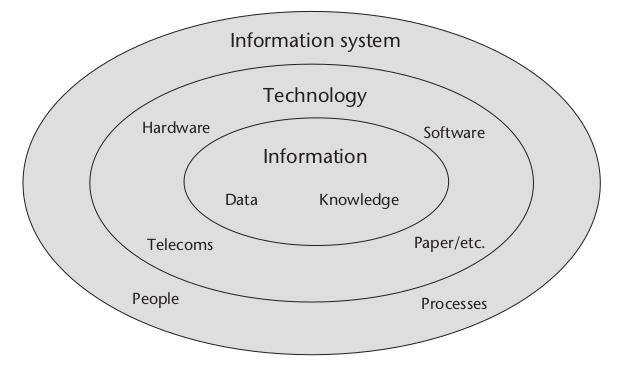
\includegraphics[width=0.8\textwidth]{e-gov-sys-as-info-sys}
	\caption[e-Government systems as information systems]{e-Government systems as information systems}
	\label{fig:e-gov-sys-as-info-sys}
\end{figure}


IT handles data to produce information. E-Government systems are information systems. At their heart lie data and information\footnote{defined as data that has been processed to make it useful to a recipient}. These are handled by digital and sometime non-digital information technologies.

But this does not make a `system'. A system is a collection of elements that works and has purpose. To understand e-government as information system, we must add in some notion of activity and purpose. That can only come if we bring people into the equation. For e-government to be working information system, it must be seen as much more than must the technical elements of IT. Instead, it must be seen to consist of technology plus information plus people who give the system purpose and meaning plus work processes that are undertaken.

Figure {\ref{fig:e-gov-sys-as-info-sys}} shows e-government systems can be described as ‘socio-technical systems’ because they combine both the social – that is, people – and the technical. This is a first indication that, when managing e-government, both social and technical (otherwise known as soft and hard) issues will have to be dealt with.



The model in Figure \ref{fig:e-gov-sys-as-info-sys} is incomplete. eGovernment systems
don’t just float around like satellites in space. Most are embedded within public
sector organizations that provide, for example,
the management systems and the organiza-
tional resources that support e-government.
These organizations also provide things
like the political and cultural milieu
within which e-government operates. Many
e-government systems also reach out to
other groups (citizens, businesses); a few
involve other public agencies. In turn, all
these groups and organizations are themselves embedded in institutional environments: a broader context of laws and values,
economic systems and technological innovations that affects both the agencies/groups
and the systems – including e-government
systems – that serve them.

Full model of e-government must embrace these factors, as shown in Figure \ref{fig:full-model-of-e-gov}.
 
 %%%%%%%%%%%%%%%%%%%%%%%%%
 %						%								
 %		FIGURE			%
 %						%
 %%%%%%%%%%%%%%%%%%%%%%%%%
 \begin{figure}[ht]
 	\centering
 	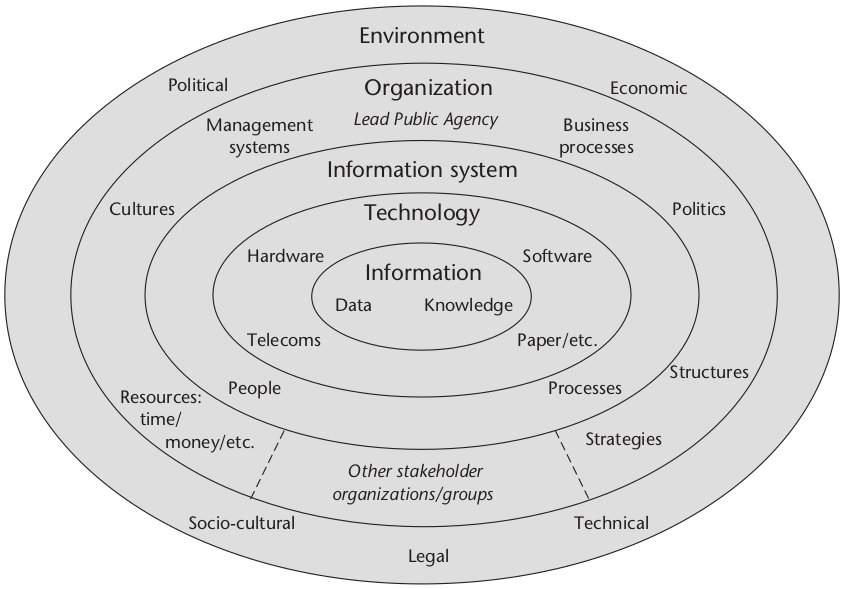
\includegraphics[width=0.8\textwidth]{full-model-of-e-gov}
 	\caption{Full model of e-government systems}
 	\label{fig:full-model-of-e-gov}
 \end{figure}


\begin{framed}
		\begin{nepali}
			\begin{center}
			\noindent Figure \ref{fig:full-model-of-e-gov} मा चित्रण गरिएकाे चित्रलाई 'onion-ring' model पनि भनिन्छ।
		\end{center}	
	\end{nepali}
\end{framed}

\subsection*{The ITPOSMO Checklist}
In fully describing and understanding an
e-government system, we could refer to every
one of the 20 separate factors identified in
Figure \ref{fig:full-model-of-e-gov}. But
that would be complex. Here, we will make more use of a slightly
simpler checklist of key items drawn out
from this `onion-ring' model:

\begin{itemize}
	\item \textbf{I}nformation: The formal information held by the digital system and the informal information used by the people
	involved with the system.
	
	\item \textbf{T}echnology: Mainly focuses on digital IT but can also cover other information	handling technologies such as paper or analogue telephones.
	
	\item \textbf{P}rocesses: The activities undertaken by the relevant stakeholders for whom the
	e-government system operates, both information-related processes and broader business processes.
	
	\item \textbf{O}bjectives and values: Often the most
	important dimension since the objectives
	component covers issues of self-interest
	and organizational politics, and can
	even be seen to incorporate formal organizational strategies; the values component covers culture: what stakeholders feel are the right and wrong ways to do
	things.
	
	\item \textbf{S}taffing and skills: Covers the number of
	staff involved with the e-government
	system, and the competencies of those
	staff and other users.
	
	\item \textbf{M}anagement systems and structures: The
	overall management systems required
	to organize operation and use of the
	e-government system, plus the way
	in which stakeholder agencies/groups
	are structured, both formally and
	informally.
	
	\item \textbf{O}ther resources: Principally, the time
	and money required to implement and
	operate the e-government system.
\end{itemize}

This ITPOSMO checklist can be used
for describing and understanding any
e-government system and stakeholder
organizational context.

In some cases, it may be important to also
describe the wider context, by expanding
the checklist to ITPOSMOO, adding an
eighth dimension:


\begin{itemize}
	\item \textbf{O}utside world: The political, economic,
	socio-cultural, technological and legal
	factors that impinge on the relevant
	e-government stakeholders.
\end{itemize}

\subsection*{The CIPSODA Checklist}
Given that e-government systems are
information systems, we can draw on one
further model/checklist to help us understand e-government. This understands an
e-government application in terms of its
information-related tasks: a process view to
go alongside the structural view offered
above. These tasks are summarized by the
CIPSODA checklist, illustrated in Figure \ref{fig:e-gov-process-view}.

The checklist of tasks can be explained in
some further detail, using the example of
part of an e-tax system:

%%%%%%%%%%%%%%%%%%%%%%%%%
%						%								
%		FIGURE			%
%						%
%%%%%%%%%%%%%%%%%%%%%%%%%
\begin{figure}[ht]
	\centering
	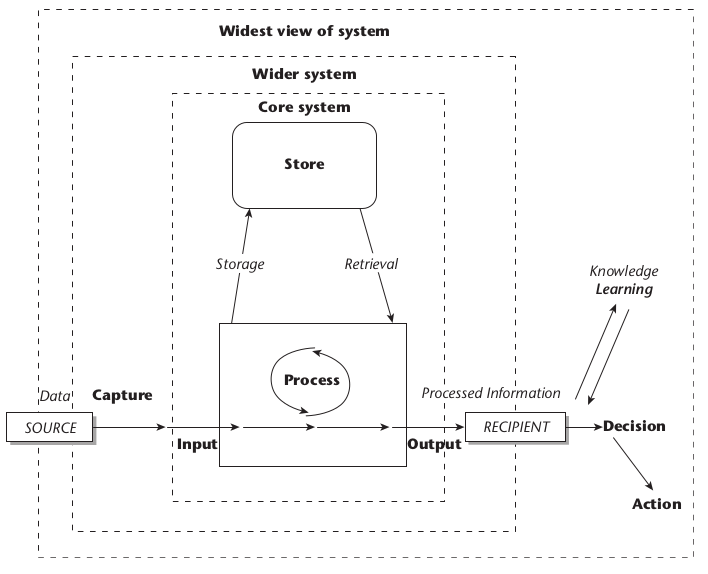
\includegraphics[width=0.8\textwidth]{e-gov-process-view}
	\caption{eGovernment systems as information systems: Process view}
	\label{fig:e-gov-process-view}
\end{figure}

\begin{itemize}
	\item \textbf{C}apture: Gathering the raw data necessary for the e-government system. The
	taxpayer obtains the basic data on their
	various sources of income.
	
	\item \textbf{I}nput: Entering the data onto the system.
	The taxpayer types the data into an
	e-form on the revenue agency’s website.
	
	\item \textbf{P}rocess: Altering the data via calculation,
	classification, selection, and so on. The
	e-tax system uses the different tax rates
	for different income types to calculate
	the total tax owed.
	
	\item \textbf{S}tore: Holding raw and processed data
	on the system. The e-tax system stores all
	details entered and calculated about this
	taxpayer.
	
	\item \textbf{O}utput: Issuing the processed data. The
	total tax calculated is displayed to the
	taxpayer.
	
	\item \textbf{D}ecision: If the processed data is useful
	enough to be seen as information, it is
	used for decision-making. The taxpayer
	determines whether to challenge or
	accept the calculated tax sum.
	
	\item \textbf{A}ction: Implementation of the decision.
	If all is well, the taxpayer authorizes payment of the tax owed.

\end{itemize}
Note there is also an eighth task implicit
within the model: the communication of
data between each of the other tasks.

While Figure \ref{fig:full-model-of-e-gov} uses an information
systems perspective to explain what an
e-government system \textit{is}, Figure \ref{fig:e-gov-process-view} explains
more what an e-government system \textit{does}.


\section{Benefits of e-Government}

\subsection{Benefits to Government}
\subsubsection{Law and Policy Making}
ICTs, especially the internet, enable gathering of model legislations and policies at international and national levels on any subject, and the experience of nations and regions in the implementation of those laws and policies. It is therefore possible to formulate new policies or modify/review existing laws and policies in a quicker time-frame and in a more informed manner.

e-Government, implemented extensively over a period, generated enough data and MIS that enable policy makers in  better decision-making.

The strength of laws and policies depends on how widely they are disseminated. Internet is the best-suited medium for this purpose. In fact, publication of all the Acts, Rules and Regulations on websites and portals is one of the common initiatives undertaken by a majority of the nations leading in the e-Government field.

\subsubsection{Regulation}
The following areas of regulation can immensely benefit from e-Government initiatives:
\begin{multicols}{2}
	\begin{itemize}
		\item Statutory registrations of companies and business under various laws
		\item Taxation
		\item Environmental regulations
		\item Police
		\item Transportation
		\item Healthcare
		\item Education
		\item Food and agriculture
		\item Industry and commerce
	\end{itemize}
\end{multicols}


Benefits in the regulatory areas could be in one or more of the following forms:

\begin{enumerate}
	\item Better compliance due to stringent tracking and monitoring systems
	\item Better revenues
	\item Better coordination between related regulatory agencies (e.g. police and transportation) due to shared databases
	\item More transparency in enforcement of laws
\end{enumerate}

\subsubsection[Electric Service Delivery]{Provision of Services-Electric Service Delivery (ESD)}
Electronic Service Delivery (ESD) is beneficial to the citizens as well as government. Following are the benefits of ESD to the government.

\begin{itemize}
	\item \textit{Better image}: Speed, efficiency, transparency and convenience arising out of ESD enhance the image of government.
	\item \textit{Cost cutting}: The automation process reduces manpower costs, besides costs of accounting, compilation, reporting and review.
\end{itemize}


\subsection{Benefits to Citizens}
The cost citizens has to incur on ascertaining the forms and procedure appropriate to the service needed, travelling to the designated government agency or to an intermediary/agent multiple time are where citizen lose their valuable time and money. By using e-government setup these costs can be reduced or eliminated.
Besides cost reduction, the other benefits to the citizen can be in the form of:

\begin{enumerate}[label=(\alph*)]
	\item increased transparency leading to reduced corruptions.
	\item better planning of personal and professional work arising out of definiteness in dealing with the government.
	\item better quality of life as a result of the use of ICT in areas such as health, education, employment, welfare and finance.
	\item easy access to information on government agencies and programmes.
	\item multiple delivery channels to choose from, thus adding to convenience and
	\item facilities like single-window and Single-Sign-On that remove the complexities of visiting multiple government agencies or websites.
\end{enumerate}


\subsection{Benefits to Business}
\subsubsection{Increased Velocity of Business}
With the digitization of the G2B interface, the velocity of business increases. Ease of filing returns and enhanced speed in securing the various permits and licenses through electronic single windows are examples.

\subsubsection{Ease of Doing Business With Government}
e-procurement provides a convenient Internet-based medium for online registration of suppliers, bidding for works and projects, and tracking the status of their award.


\section{e-Government Stages of Development}
The theoretical progression of e-Government in any country or state is along \textit{four stages} which indicate the extent of benefits that the stakeholders get through the e-Government projects prevalent in that country or state. These are represented schematically in Figure {\ref{fig:e-gov-dev-stages}}.


%%%%%%%%%%%%%%%%%%%%%%%%%
%						%								
%		FIGURE			%
%						%
%%%%%%%%%%%%%%%%%%%%%%%%%
\begin{figure}[ht]
	\centering
	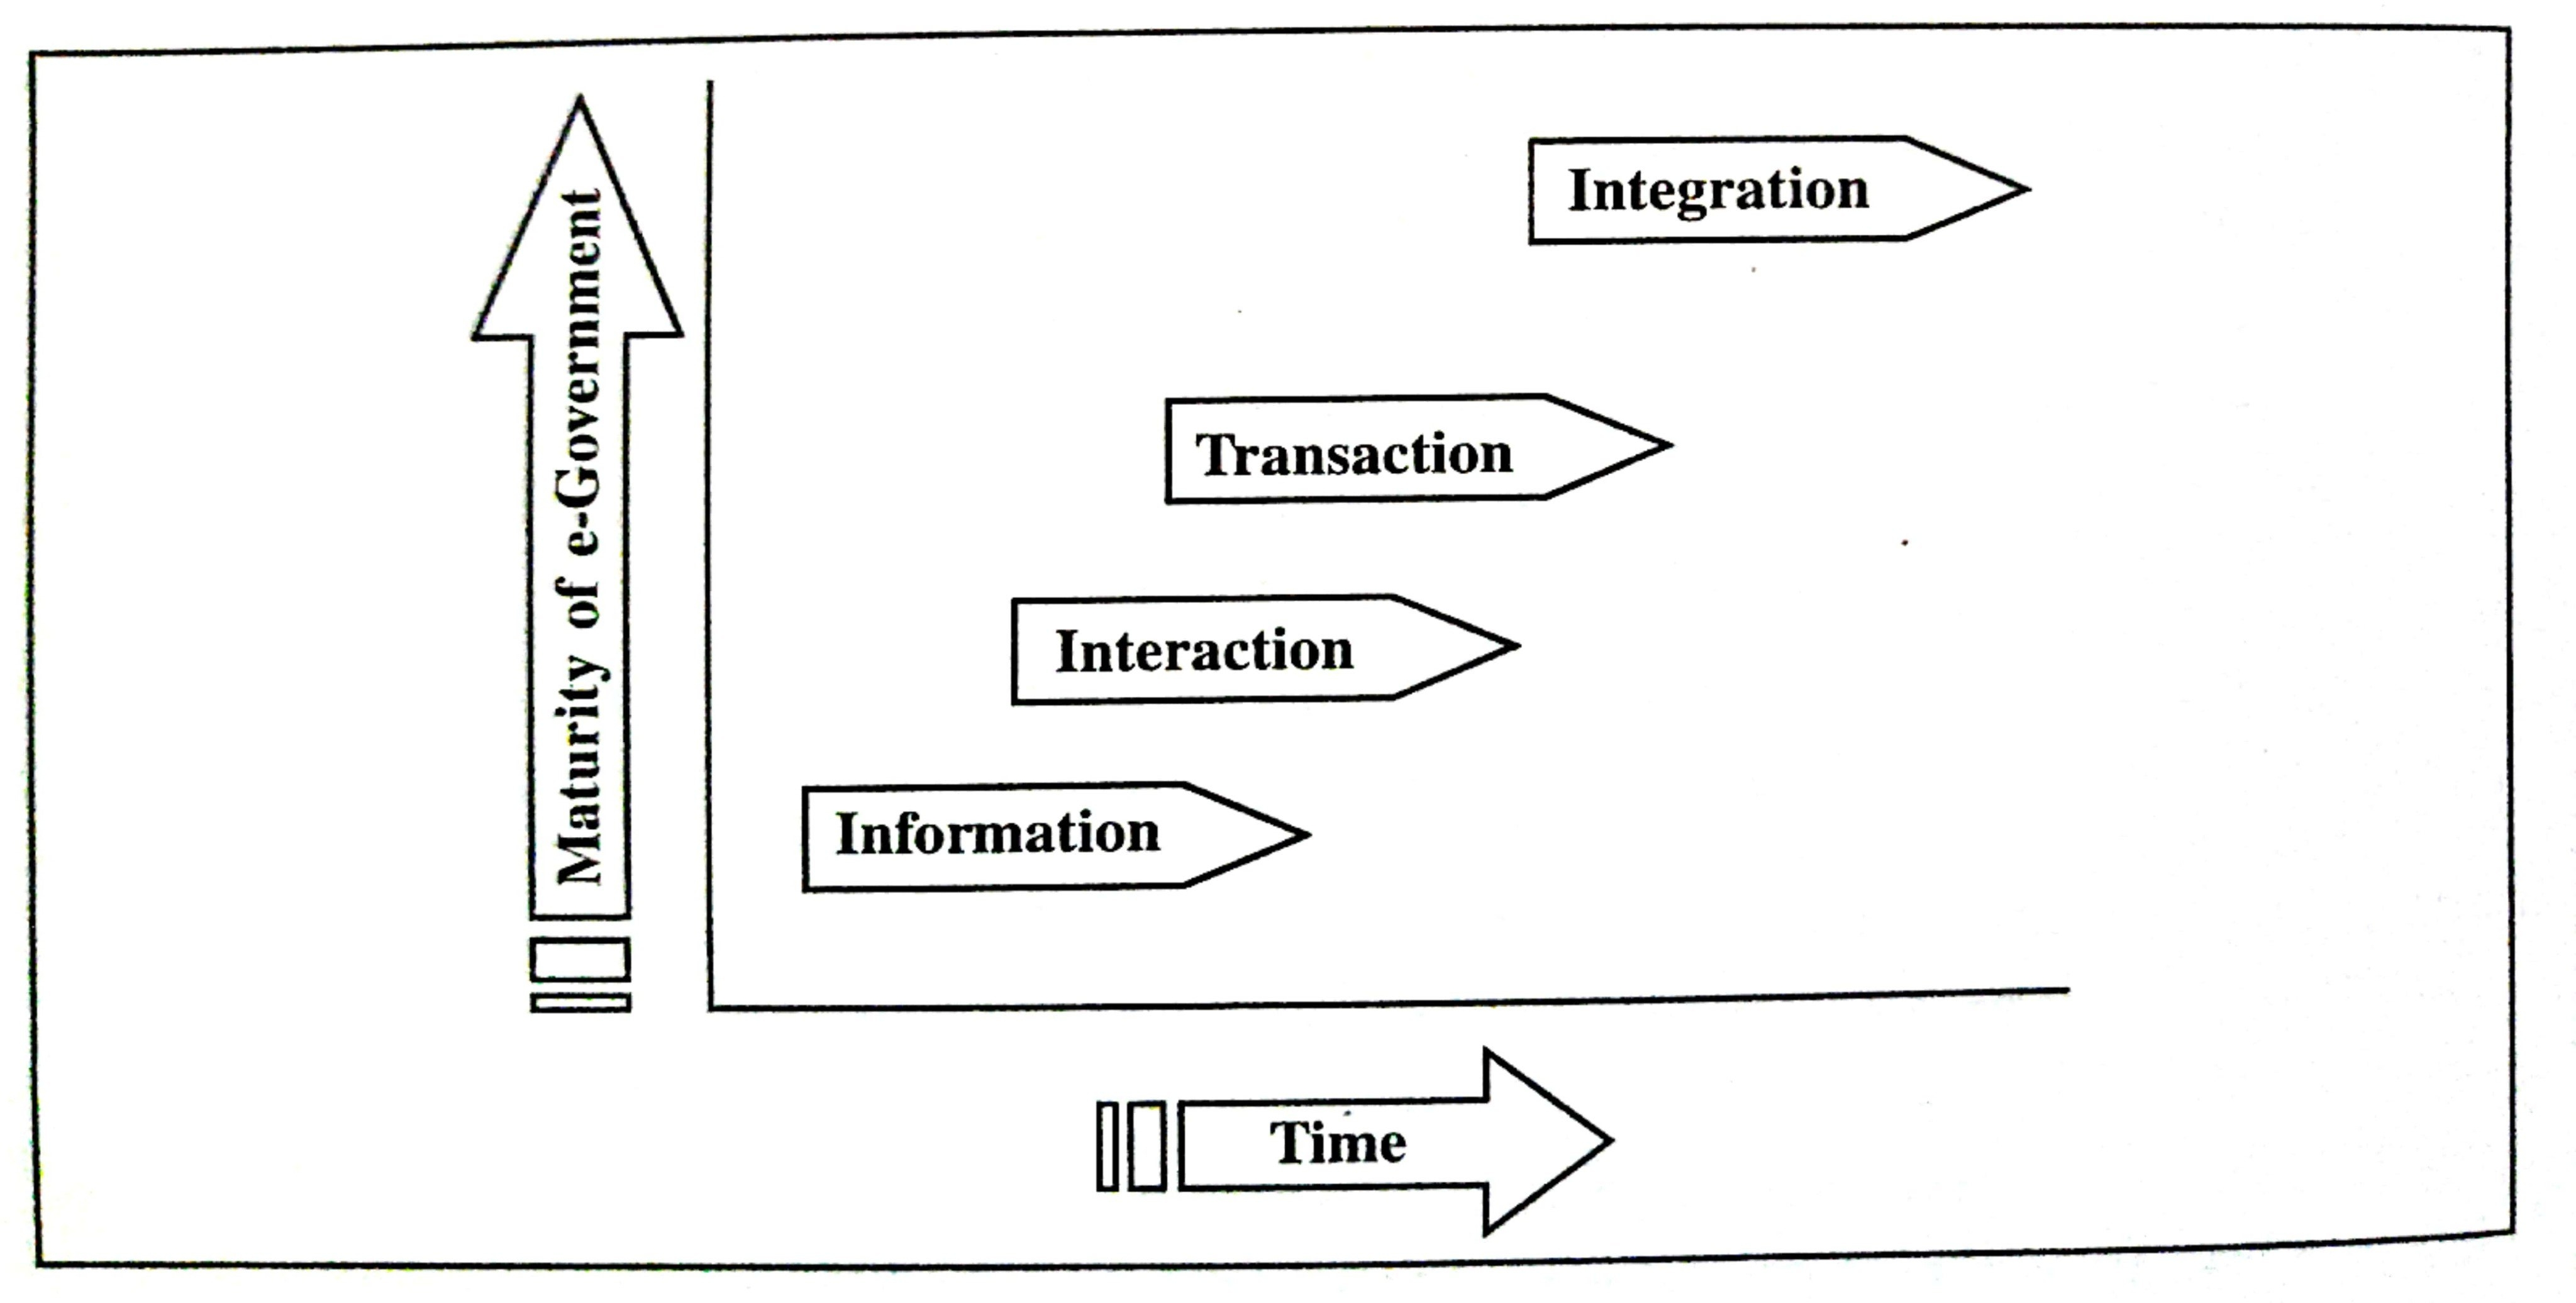
\includegraphics[width=0.8\textwidth]{e-gov-dev-stages}
	\caption{e-Government systems as information systems}
	\label{fig:e-gov-dev-stages}
\end{figure}

\subsection{Information}
This is the initial stage of web presence. A few websites are launched that contain limited and static information, which is updated more frequently with increasing usage and customer pressure. The information may be limited to basic functions, facts and figures and contact details of government departments and agencies. The information stage does not call for any efforts at `Computerization’ of the backend.

\subsection{Interaction}
In this stage, the citizen can \textit{interact} with the government agencies in a ‘one way street’ manner. The citizens can download forms, file forms, returns and complain online, with government agencies. This stage calls for building capacity and systems in the backend government agencies to receive the request send by the
citizen online and to process in sequential and accountable manner. The interactive website reduce the tedium of the citizen partially by enabling them to save at least one step in dealing with government agencies.

\subsection{Transaction}
This is a much more difficult stage to reach. In the transactional stage, the citizens can go through a full cycle of fulfillment of their request. It is a two-way street.  Complete and secure transactions such as online payments for utility bills, taxes, fees, registration, renewals, obtaining permits, licenses and certificates are typical examples of transactions. e-Procurement, Online customs clearance, single window and single-sign-on are more sophisticated examples of this stage. This requires extensive system study, establishing data centers, disaster recovery and management system. The services have to be delivered on a $24\times7$ basis, the services should be citizen centric and should reflect the transformation that is the hallmark of e-government.

\subsection{Integration}
This is yet the Utopian\footnote{An idealistic (bust usually impractical)} stage of e-government. This stage envisages\footnote{Form a mental image of something that is not present} offering government information and services in an integrated manner not only from government view but also from citizen and business side. The key events in the citizen’s life are- birth, admission to school, admission to college/university, employment, housing, marriage, shifting of job/house, medicare, senior citizenship and death. The key events of business are registration of a firm/company, securing all clearances for setting up business/industries, filing of returns, payment of taxes and winding up.


\section{Online Service Delivery and Electronic Service Delivery}
\subsection{Online Service Delivery}
Online service delivery is the system of e-government by providing information and other various services through the means of Internet. Most services can be provided by online and services are available anywhere anytime but only the limitation is lack of availability of Internet to all places and not every citizen are computer-literate. Also, government have to initially invest large budget for establishing, utilizing and securing ICT system for online service delivery.


\subsection{Electronic Service Delivery}
Electronic service delivery means providing the services to citizen and business
electronically without Internet i.\ e.\ Television, Radio, Telephone, SMS system etc.



\newpage\thispagestyle{empty}








 % ch-1: Introduction 
\chapter{Public-Private Partnership for e-Government}
Public Private Partnership (PPP) is a different method of procuring public services and infrastructure by  combining the best of the public and private sectors with an emphasis on value for money and delivering quality public services.

The concept of PPP has been brought into operation in the construction and operation of public infrastructure projects like bridges, airports, highways, hospitals, etc.

PPP is a reform that is a `generation next' to privatization. Privatization is the process of involving the private sector in the ownership and management of of ongoing and existing projects and business of the public sector. In PPP, the private sector partner is induced into a project right from the stage of initiation to completion and management.

\section*{Why PPP for e-Government?}

\subsection*{Combining Accountability With Efficiency}
\begin{itemize}
	\item PPP for e-government would combine the accountability and domain expertise of the public sector with the efficiency, cost-effectiveness and customer-centric approach of the private sector.
\end{itemize}

\subsection*{Complexity and Size of e-government}
Since many agencies are managed by government, its strucute is huge and complex but government does not have sufficient resource to manage such complexities, private sector could raise \textit{unlimited} resources.

\subsection*{Pace of Implementation}
Government cannot plan for implementing projects one after the another because it would be almost impossible to maintain all the projects smoothly. 

In order to maintain a high pace in implementing e-government, government should join hands with the private sector.

\section{G2B Project}
\begin{itemize}
	\item e-procurement
	\item G2B portal
\end{itemize}

\section{G2C Project}
\begin{itemize}
	\item Citizen service portals
	\item Integrated service centers
	\item Agency service centers 
	\item Networks of kiosks
\end{itemize}

\section{PPP Forms}
PPP can be of different forms, depending on the shares of government and the private sector in the investment, control as also on the strategic nature and commercial viability of the project/initiative. Different models of PPP are described in the following section.

\subsection[JV Model]{Joint Venture (JV) Model}
In this model, an SPV (Special Purpose Vehicle) is formed to undertake the e-government project and/or to provide e-services. The joint venture can be led by the government or by the private sector depending upon the strategic nature and sensitivity of the domain.

A JV model is preferred option for projects involving
\begin{enumerate}[label=(\alph*)]
	\item delivery of services, which are basic and permanent in nature e.\ g.\ a country portal.
	\item setting up of infrastructure with steady returns envisaged in long term e.\ g.\ a State Data Center.
	\item handling of sensitive data and information relating to citizen, businesses and government and
	\item close coordination with and cooperation from  a host of government agencies.
\end{enumerate}

In Joint Venture the government share varies from 51\% to 11\% which can be in cash but also can be in the form of tangible assets like land, building, equipment or in the form of intangible assets like right to access government information and databases for providing e-services.

In Nepal, some hydro projects are under construction on JV model between government and public.

\subsection[BOO Model]{Build-Own-Operate (BOO) Model}
\begin{itemize}
	\item In this model, the selected partner designs, develops and implements the projects, most often, entirely at its cost and operates the system for a pre-specified period called \textit{concession} period.
	\item The revenue model of the project is either based on transaction charges (paid by the citizen or the government) or EQI/EMI(Equated Quarterly Installment/Equated Monthly Installment) paid by the government to the operator/service provider.
	\item The BOO model is suitable for projects that involve setting up of physical infrastructures such as service center(s) for delivering services to the citizens. 
\end{itemize}

Example are projects related to:
\begin{multicols}{2}
	\begin{itemize}
	\item driving licenses
	\item vehicle registration
	\item provision for integrated services
	\end{itemize}
\end{multicols}

The important aspects in drafting Request For Proposal (RFP) for BOO Project are:
\begin{enumerate}[label=(\alph*)]
	\item to determine period of the arrangement during which partner is authorized to deliver the services, and
	\item The bid parameter dealing with transaction charges and/or EQI/EMI to be quoted by the competitive bidders.
\end{enumerate}

The BOO model is usually adopted in e-Government projects that deploy time-tested technologies and have a fairly reliable revenue mode.

\subsection[BOOT Model]{Build-Own-Operate-and-Transfer (BOOT) Model}
This is almost identical to BOO except that the government exercises ownership of the assets created by the partner at the end of the project. 

This model is adopted where the technology is time tested and the ICT assets are expected to outlast the concession period.

\subsection[ASP Model]{Application Service Provider (ASP) Model}
In this model the government contracts to avail\footnote{Take or use} the services of the partner for delivery of services as per mutually agreed service levels and commercial terms. The revenue model is typically transaction based. The ASP model is suitable to e-government initiatives that involve:

\begin{enumerate}[label=(\alph*)]
	\item a requirement to launch the services in a short time frame.
	\item the technology is not complex and is widely accepted and practiced in the private sector, and
	\item the nature of information is not so sensitive or critical to governance.
\end{enumerate}

Examples of ASP model are:
\begin{enumerate}[label=(\roman*)]
	\item design and hosting of websites that provide fairly static information to the citizens.
	\item provision of simple services like downloading/filing of forms, and
	\item provision of MIS services in the G2G arena to the government agencies.
\end{enumerate}

Most often, the ASP model is useful to leverage the existing ICT infrastructure and management skills already established by service providers. This creates a win-win situation by enabling the optimum utilization of the ICT infrastructure already setup in the private sector and thereby reducing the transaction cost to the government/citizen. The ASP model also saves the government agencies of the hassles of designing complex technology and partnership models.


\section{Issues in PPP for e-Government}
Though there are many advantages of PPP, if proper negotiation is done. But both have their own interest to earn more benefits which may threaten PPP relationship. Some issues are:

\subsection{Lack of Congruence in Objectives}
The degree to which the public and private sector partners align themselves along sharing the investment and control. Both must commit to developing an understanding of each others objectives but failing in such understanding and only focus on own interest creates lack of congruence in objectives and may fail the relationship.

\subsection{Risk and Control}
In every business there is risk and control mechanism. Most often, governments attempt to transfer risk to the partner without passing on the related control quoting ‘public interest’ as the reason.

\subsection{Clash of Cultures}
The organizational culture of private and public sector differ widely in all parts of the world which is bound to result in conflicting situation. The private partners tend to look at the government employees as bureaucrats with antiquated ideas that have outlived their time. 

\subsection{Monopoly}
In some cases, only one partner is suitable in areas such as e-procurement, country or state portal, data center, gateway and the like. This is likely to result in a situation of monopoly- the monopoly of the state being replaced with the monopoly of the private partner and more importantly, \textit{monopoly of a particular technology}.

The following methodology is recommended to mitigate its impact.

\subsubsection*{Operational Monopoly}
The \textit{operational monopoly} can be handled by defining the commercial features of the contract unambiguously while notifying the project to an open bid. The following factors are to be considered:
\begin{enumerate}
	\item Projected customer base and transaction volume
	\item Length of the concession period
	\item Fee structure of the existing services
	\item Price elasticity of the new services
	\item Capacity for growth.
\end{enumerate}

\subsubsection*{Technology Monopoly}
The \textit{technology monopoly} can be mitigated by prescribing open standards in conformity with the technology architecture approved by the government and ensuring that there is scope for developing interfaces with other systems that may be developed concurrently or in the future.

\section{Citizen-Centric Approach to e-Government}
Citizen-centric eGovernment services are designed to deliver increasingly costeffective, personalized and relevant services to citizens, but also serve to enhance
the democratic relationship, and build better democratic dialogue, between citizens
and their government, which then enhances the practice of citizenship within
society.

\begin{enumerate}
	\item It is necessary to look at e-government from the citizen or customer’s point of view and design the front-end and the back-ends to the extent required to fulfill the requirement of citizen/customer, i.\ e.\ e-government initiatives should not be system driven or supply-driven but should be demand-driven.
	
	\item The e-Government projects can be classified as \textit{core} and \textit{non-core}. Core projects are those, that can be used by all departments across the state and with significant impact on key stakeholders like citizen, businesses and employees.
	
	\item The e-Government projects  can also be categorized as \textit{commercial} and \textit{non-commercial}. Commercial projects are those that permit a viable public-private partnership model to be implemented with the least outgo from the public exchequer\footnote{The funds of a government} for implementation.
\end{enumerate}

\newpage\thispagestyle{empty} % ch-2: Public-Private Partnership for e-Government
\chapter{ICT Infrastructure for e-Government}


\section{Network infrastructure}
Network infrastructure means the infrastructure that helps to connect computing devices within the office, other offices or connected to the world using internet. Network infrastructure includes networking devices like switch, router, networking cables, internet, intranet etc.

\section{Computing Infrastructure}
Computing infrastructure means availability of computers, laptops and other related devices which are needed for day to day computerized work in the office and providing various services.

\begin{itemize}
	\item While on one end, government needs large computing infrastructure to develop and deliver e-government services on continuous basis, infrastructure is also needed at the end of citizens to derive the benefits of these services.
	
	\item Again, like communication infrastructure, there is a high order of disparity in availability, affordability of computing devices in urban and rural areas, particularly in developing countries.
	
	\item Further, in rural areas, due to lack of basic infrastructure such as electricity, telephony, it may not be worthwhile for the people to have computers, even if they could afford it.
	
	\item To extend the reach of government services and address the wide range of citizens, governments all over the world are setting up common / shared / community infrastructure in the form of community information center, Internet kiosks etc.
	
	\item Government should also consider, making their services accessible from various other media/devices such as basic telephones, mobiles, cable TV network, PDAs and many other hands held devices.
	
\end{itemize}
\section{Data Centers}
Data centers is a place where many dedicated computers, servers and storage are available for mass storage of data. All public or private offices can backup their important data in secure way in least cost and prevent any loss of their data from disaster or failure of their system. In Nepal there are two data centers GIDC and DOIT. 

\begin{itemize}
	\item In the era of e-governance, government is expected to deliver its services to the citizens on $ 24\times7 $ bases. To achieve this, the government has to set up a sound and stable infrastructure operational round the clock.
	
	\item Internet Data Center is a facility which provides extremely reliable and secure infrastructure for running Internet operations on a $ 24\times7 $ basis. It shall not at all be cost effective if each department starts setting up its own data center as running a high class Internet Data Center needs a lot of recurring resources.
	
	\item It is, therefore, suggested that the government may set up a high grade Data Center at a National level to be used by all entities of the government.
	
	\item All departments should, in turn, establish high speed connectivity with the data center so that they can manage their applications from their own premises in a secured manner.
	
	\item In cases where the country is large and the government feels that one Internet Data Center may not suffice, it could decide to set up multiple Data Centers.
	
	\item However, the number of data centers should be optimized to the extent possible primarily due to the high recurring operative costs as well as scarcity of skilled resources.
		
	\item As the pace of e-government picks up nationwide, besides delivery of services, Government may also have to set up data centers to share the large scale/special purpose resources for development of the systems.
\end{itemize}


\section{e-Government Architecture}
There is no commonly agreed definition of e-Government architecture. The result is how the different countries states it. E-government Architecture generally consists of three components: 
\begin{multicols}{2}
	\begin{enumerate}
		\item Service Architecture
		\item Process Architecture and 
		\item Data Architecture
	\end{enumerate}
\end{multicols}


\subsection{Service Architecture}
Describes a lot of services offered by the Government, processes to be followed for each service, Concerned Department(s), relation/dependence on other services etc. Services could be like Vehicle Registration, Passport Issuance, Caste Certificate, Payment of Tax, etc.

 \subsection{Process Architecture}
 
 \begin{enumerate}[label=(\roman*)]
 	\item Lists the various processes to be followed for rendering different services, independent of their association with one or more services. 
 	\item These processes are then further grouped in various categories and detailed rules/procedures are defined for executing each of the processes. 
 	\item This brings a lot of standardization across services and promotes interoperability as well as reuse of process components. 
 	\item Processes could be Content Management, Citizen Registration, Personalization, Online Form Submission, Electronic Payment etc.
	 \end{enumerate}

\subsection{Data Architecture}

 \begin{enumerate}[label=(\roman*)]
 	\item Deals with the data associated with various Government Services, as described in service architecture. 
 	\item In Data Architecture, we enlist all the data elements needed/associated with above service and then define meta-data about each data element.
 	\item This meta-data information includes the standard Nomenclature for each data elements, their type, size, format, default value, valid value range, owner etc. 
 	\item Use of such a standard definition by all government applications shall facilitate interoperability among various applications as well their integration which shall go long way in delivery of integrated / one stop services to the citizens and businesses.
 \end{enumerate}


\section{Interoperability Framework}
\begin{itemize}
	\item The Interoperability Framework aims to define the set of specifications to facilitate Government systems to communicate and interoperate with other systems, both within Government and external to it, efficiently and effectively.
	\item By bringing together the relevant specifications under an overall framework, ICT management and software developers have a single point of reference whenever a need arises to locate the required interoperability specifications that should be followed for a specific project. 
	\item By adopting these interoperability specifications, system designers can ensure interoperability between systems while at the same time have the flexibility to select different hardware, systems and application software to implement solutions.
	\item In order to attain this objective, the Government needs to be perceived as a single entity, with seamless flow of information across individual ministries and departments as necessary.
	\item Framing of policies and specifications for Interoperability Framework should be followed up with provision of support, guidance on best practices, toolkits and agreed schema. 
	\item The entire strategy to implement good e-government should be viewed in long-term perspective and hence must be supported by vigorous processes. 
	\item The development of Interoperability Framework must therefore be reviewed and updated on a continuous basis.
\end{itemize}

\subsection*{e-Government Interoperability Framework (e-GIF)}
e-GIF is a set of guidelines and technical specifications, designed to promote interoperability between various e-government systems, though developed independently by various agencies. In the words of Mr. Douglas Alexander, in his foreword to the e-GIF Framework (Version 5.0),

\begin{quotation}
	\noindent \say{in terms of e-service delivery, compliance with the (e-GIF) Framework is essential for the public good... the Framework aligns government with the rest of the industry and serves as a basis for reducing the costs and risks associated with carrying out major IT projects}
\end{quotation}

The key policy decisions that have shaped the e-GIF are as follows:

\begin{itemize}
	\item Align with the \textbf{Internet technologies} and specifications, for all public sector information systems.
	\item Adopt \textbf{XML} as the primary standard for data integration and presentation tools,
	\item Adopt the \textbf{browser} as the key interface.
	\item Adopt \textbf{metadata} to government information resources.
	\item \textbf{Mandate} e-GIF throughout the public sector.
\end{itemize}

The e-GIF specifications are driven by integrability, market-support, scalability and openness of the technologies prescribed. The scope of e-GIF specifications has been limited to four key ares of technology, viz.

\begin{itemize}
	\item Interconnectivity,
	\item data interpretation,
	\item e-services access  and 
	\item content management
\end{itemize}

\newpage\thispagestyle{empty}
 % ch-3: ICT Infrastructure for e-Government
\chapter{e-Government Readiness}
e-government takes root and grows when a country, state or agency is \textit{e-ready}.

\subsection*{e-Readiness}
According to Harvard Business School,
\begin{quotation}
	\noindent an e-Ready society is one that has the necessary physical infrastructure (high bandwidth, reliability and affordable prices). It should also have an integrated, current ICT's throughout business communities (e-commerce, local ICT sector), and government (e-government). Other important aspects are strong telecommunications competition, independent regulation with a commitment to universal access, and no limits on trade or foreign investment.
\end{quotation}


In short, e-readiness measures a nation's capacity to participate in the digital economy. While e-readiness is a larger concept that measures how a nation comprising citizens, businesses and government takes advantage of the digital revolution, `e-government readiness' relates to how the process involving the government are transformed using the tools of ICT. In other words, e-readiness touches upon the state of all interface - G2G, G2B, B2B, B2C and C2C, while e-government readiness is concerned with only the first three interfaces.


\section{e-Readiness framework}


Following list shows component, sub-component and indicators of e-readiness.

\begin{enumerate}
	\item \textbf{Policy}
	      \begin{enumerate}
		      \item ICT Policy
		            \begin{itemize}
			            \item Communications Policies
			            \item Policy on ISP
			            \item Incentives to ICT Industry
			            \item Recognition of Quality
			            \item Facilitation of Growth \& Promotion of Exports
		            \end{itemize}

		      \item E-Government Policy
		            \begin{itemize}
			            \item E-Government Vision
			            \item Prioritization of Services
			            \item PPP Policy
			            \item Policy on ESD (Electronic Service Delivery)
		            \end{itemize}

		      \item Architecture \& Standards
		            \begin{itemize}
			            \item Functional Architecture
			            \item Technical Architecture
			            \item Technical Standards
		            \end{itemize}

		      \item Security Framework
		            \begin{itemize}
			            \item Security Policy
			            \item Privacy
		            \end{itemize}

		      \item Regular Framework
		            \begin{itemize}
			            \item Cyberlaw
			            \item IPR Protection
		            \end{itemize}
	      \end{enumerate}

	\item \textbf{Infrastructure}
	      \begin{enumerate}
		      \item Networks
		            \begin{itemize}
			            \item National Backbone(s)
			            \item Distribution Networks
			            \item LANs \& WANs
			            \item Satellite \& Wireless Networks
		            \end{itemize}

		      \item Access
		            \begin{itemize}
			            \item PC Penetration
			            \item Internet Penetration
			            \item Last Mile Connectivity
		            \end{itemize}

		      \item ICT Hardware
		            \begin{itemize}
			            \item Data Center
			            \item e-Government Gateway
			            \item Payment Gateway
			            \item Public Key Infrastructure
		            \end{itemize}
	      \end{enumerate}

	\item \textbf{Resources}
	      \begin{enumerate}
		      \item Political Resources
		            \begin{itemize}
			            \item Leadership \& Vision
			            \item Continuity of Support to ICT Sector
		            \end{itemize}

		      \item Human Resources
		            \begin{itemize}
			            \item IT Education \& Training Institutions
			            \item Expenditure on R\&D in ICT
		            \end{itemize}

		      \item Employee Resources
		            \begin{itemize}
			            \item Champions of ICT
			            \item Chief Information Offices
			            \item Access to PC \& Internet at Office
		            \end{itemize}
	      \end{enumerate}

	\item \textbf{Usages}
	      \begin{enumerate}
		      \item Usage by Citizen
		            \begin{itemize}
			            \item e-Mail \& Internet Usages
			            \item e-Literacy

		            \end{itemize}

		      \item Usage by Businesses
		            \begin{itemize}
			            \item e-Commerce
			            \item e-CRM; e-SCM
			            \item e-Procurement in B2B \& G2B Areas
		            \end{itemize}

		      \item Employee Resources
		            \begin{itemize}
			            \item No.\ of Websites/Portals
			            \item No.\ of e-Services; e-Transactions
			            \item No.\ of e-Government Projects
			            \item Extent of G2G Usage
		            \end{itemize}
	      \end{enumerate}
\end{enumerate}

The e-readiness framework consists of assessing readiness along four fronts:
\begin{itemize}
	\item policy,
	\item infrastructure,
	\item resources and
	\item usages.
\end{itemize}

Each of the four components consists of 3-5 sub-components that enable a deeper understanding of the state of each of the major components. A set of 43 indicators is suggested as a drilled down of the sub-components to enable quantitative and qualitative assessment of e-readiness.

It is possible to develop a methodology to asses the e-readiness of a country or a state, through a structured questionnaire, administered to a representative sample population of the citizens, companies and government agencies and supplementing the same with the macroeconomic data available with regulatory bodies, research institutions and industry associations. The following questionnaire is suggested as a starting point. It can be improved upon and customized to suit varying circumstances.

\subsection{Policy}
\subsubsection*{ICT Policy}
\begin{itemize}
	\item Does the country (State) have an ICT policy? How old is it? How contemporary is it?
	\item Does the country (State) have a telecommunications policy? Does it promote competition?
	\item Does the country have a policy on ISPs (Internet Service Providers)?
	\item Does the State provide sizeable incentives to the ICT sector in the form of tax concessions, allocation of state lands at a concession?
	\item Does the state promote exports of ICT products and services?
	\item Are there awards instituted for excellence in ICT sector?
\end{itemize}

\subsubsection*{e-Government Policy}
\begin{itemize}
	\item Is there a document that specifies the state's e-government vision and strategy?
	\item Is there clarity on the priorities in implementation of e-government? Is there a 5- or 10-year perspective plan, broken down into annual action plans with clear quantitative and qualitative targets?
	\item Has the state laid down a transparent policy on Public-Private Partnership for e-government? How many PPP initiatives are ongoing/completed?
	\item Is there a policy on ESD that creates an open framework for development of multiple channels?
\end{itemize}


\subsubsection*{Architecture and Standards}
\begin{itemize}
	\item Has the government published a document that sets out the functional architecture or business process architecture?
	\item Is there a document that prescribes standards in all the technology areas like application development, databases, middlewares, networks, storage, etc.\ ?
	\item Has the government published a technology architecture that is based on open standards and permits development of IT systems in an interoperable manner and a seamless integration with national and global systems?
\end{itemize}



\subsubsection*{Regulation}
\begin{itemize}
	\item Is there an overarching cyberlaw at the national level that confers legal status to electronic transactions and documents?
	\item Is there a law on regulation of digital signatures and encryption?
	\item Is there a law to protect Intellectual Property?
	\item Is there a law on privacy that protects the information of citizens and businesses captured by the government and private agencies, against unauthorized use? 
	\item Is there a statutory regulator for the telecom sector that promotes competition?
	\item Is there an effective legal machinery to tackle the problem of piracy of ICT products?
\end{itemize}

\subsection{ICT Infrastructure}
\subsubsection*{Networks}
\begin{itemize}
	\item Are there at least two major national networks that connect all the major cities? 
	\item Are there two or three distribution networks to connect all towns and all villages? 

	\item Do the federal and state governments and their agencies have WANs of their own? 

	\item Do the public offices and enterprises have LANs that use State-of-the-art switches and routers? 
	\item Is there effective usage of satellite and wireless networks in government and business?
\end{itemize}

\subsubsection*{Access}
\begin{itemize}
	\item What is the PC penetration in terms of a PC per 1000 population? What percent of households have PCs?

	\item What is the Internet penetration in terms of Internet accounts per 100 of population?

	\item What is the technology adopted to connect the last mile? Dial up? Optical Fiber Cable? Wireless?
\end{itemize}

\subsubsection*{ICT hardware}
\begin{itemize}
	\item How many data centres are established in the country?

	\item Does the country have an e-government gateway?

	\item Is there an e-payment getaway?

	\item Does the country have a PKI?
\end{itemize}

\subsection{Resources}

\subsubsection*{Political Resources}
\begin{itemize}
	\item Is there a document at national level that describes the ICT vision of the country?
	\item Is there a political consensus on the promotion of ICT in the country? 
	\item Are there champions of ICT and e-government at the national and state levels among the political executives?
	\item In the last 10 years, how often has political support been given to the ICT sector?
\end{itemize}

\subsubsection*{Human Resources}
\begin{itemize}
	\item Is the country or state self-sufficient in IT graduates? 

	\item How many IT training institutes operate at the national level, outside the formal education system?

	\item What is the percentage of turnover spent on R\&D in the ICT sector?

	\item How many institutions of excellence that have national and international reputation exist in the IT sector?
\end{itemize}

\subsubsection*{Employee Resources}
\begin{itemize}
	\item What percentage of enterprises (other than SMEs) have qualified Chief Information Officers?
	\item What is the percentage of government enterprises- federal and state-having CIOs?
	\item What is the percentage of employees having access to a PC and Internet at office — in the public and private sectors?
\end{itemize}

\subsubsection*{ICT Resources of Private Sector}
\begin{itemize}
	\item How many ICT companies are active in the country/state?
	\item How many of them partner the government?
\end{itemize}

\subsubsection*{Financial Resources}
\begin{itemize}
	\item What is the total ICT budget of the Federal, State and local governments? 
	\item What is the annual IT expenditure of the private sector?
\end{itemize}


\subsection{Usage}
\subsubsection*{Usage by Citizens}
\begin{itemize}
	\item What is the rate of e-literacy among the citizens?

	\item What is the extent of e-mail usage and Internet browsing among citizens?

	\item What percentage of citizens use e-service over the Internet in preference to over-the-counter?

	\item What is the share of e-buying in the total consumer spend?
\end{itemize}

\subsubsection*{Usage by Business}
\begin{itemize}
	\item What is the share of e-commerce in the overall business?

	\item What percent of major industries and business have adopted eCRM, eSCM and e-procurement?

	\item What is the level of trust in the net among business people?
\end{itemize}

\subsubsection*{Usage by Government}
\begin{itemize}
	\item What percent of G2C and G2B services are offered electronically?
	\item What percent of G2G, G2B transactions occur electronically?
	\item How many enterprise-wide e-government projects are operational?
	\item What percent of government agencies have websites/portals that are regularly updated and used by the citizens?
	\item What percent of government employees use PC and Internet for official work?
\end{itemize}

It is a long and elaborate questionnaire. The answers to most of these questions can be qualitative to begin with. Where quantitative responses are required, a sample survey would be the best. It is advisable to adopt a system of weightages to assess the overall e-readiness of a country/state or enterprise.

\section{Steps to e-Government Readiness}
10- Step process to e-government readiness that can act as a guide for improving the score of e-government readiness. It is not necessary to follow the 10 steps sequentially. Some of them can be implemented in parallel. Each step may be broken down into a set of tasks and pursued for effective results. In fact, some steps and components, such as design of architecture, the CIO program, setting up of a state data center and gateway, are themselves very large initiatives.

\begin{steps}
	\item Articulate the e-government vision and strategy. Prepare a five-year perspective plan.

	\item Review the Telecommunication policy, to promote an open, competitive environment for creation of national and sub-national networks.

	\item Prepare a list of G2C and G2B services that citizens and businesses need to be provided electronically.

	Prioritize the services.

	Announce a policy on electronically services delivery.

	\item {\label{stp:four}}Design Functional and Technology Architectures that are aimed at delivering the e-services.

	Prescribe standards for security.

	\item Initiate statewide e-government projects adopting the pilot approach. Ensure these are part of the ‘big picture’ developed in {\ref{stp:four}}.

	\item Design and implement an appropriate CIO program.

	Implement change management programs across all major government agencies.

	\item Ensure that all government agencies earmark\footnote{designate (funds or resources) for a particular purpose} 2-5\% of their budget to e-government.

	Announce a PPP policy for e-government and take up a few projects adopting the PPP
	Model.

	\item Establish a government–wide WAN for data, voice and video for G2G applications, adopting a PPP model.

	\item Enact a cyber law that gives a legal validity to all electronic transactions and records and permits use of digital signatures for authenticating messages and documents.

	Publish polices on security and privacy for e-government.

	\item Establish data centers for e- government using the PPP model.

	Design and establish an e-government gateway at the State Data Center.
\end{steps}

\section{Issues in e-Government Readiness}
Getting a country into a stage of e-readiness requires a mulltipronged\footnote{having several distinct aspects or elements} effort. While it is possible to adopt a structured approach, it is fraught\footnote{(of a situation or course of action) filled with or likely to result in (something undesirable)} with several problems. It is necessary to look at three issues which are crosscutting in nature:
\begin{multicols}{2}
	\begin{itemize}
		\item people readiness,
		\item reform readiness, and 
		\item readiness for sustainability.
	\end{itemize}
\end{multicols}



\subsection{People readiness}
We can program processes. We cannot program people. There lies the problem — in getting people ready for e-government. People readiness has four stages of evolution.
\begin{multicols}{2}
	\begin{enumerate}
	\item Readiness to \textit{think}
	\item Readiness to \textit{learn}
	\item Readiness to \textit{act}
	\item Readiness to \textit{transform}.
\end{enumerate}
\end{multicols}


\subsubsection{Readiness to Think}
Readiness to think of e-government is to do with the change of mindset and is by far the most difficult one to achieve.

\subsubsection{Readiness to Learn}
Readiness to learn is easier to come by. It can be ushered\footnote{show or guide (someone) somewhere.} in through a set of attractive training programs coupled with visits to successful e-government projects and interaction with people running the project and those benefiting from it.

\subsubsection{Readiness to Act}
Readiness to act is a hands-on exercise. It is believed that giving a person a PC and exposing to the Net is a good way to initiate him or her into the e-world and getting people hooked on to `Act'.

\subsubsection{Readiness to Transform}
Readiness to Transform is the final stage where people in the organization start acting as teams, willing to spare an extra hour to improvise, improve, innovate and transform the workplace and the service center.

\subsection{Reform Readiness}
e-government efforts end up as `old wine in new bottle' unless these are accompanied by an urge to transform the way government functions and treats its customers. This is possible through an extensive exercise to reform the processes and the legal provisions underlying them. Reform is triggered by the need to introduce new services and to provide the existing services in a new way to the citizens, in a manner that is convenient and cost effective from the citizen's viewpoint.


\subsection{Backend Readiness vs. Front-end Readiness}
One of the classic conflicts that arises in the course of a serious implementation of e-government is the one between `backend readiness' and `front-end readiness'. By `backend readiness' we mean the following tasks:

\subsubsection*{Developing Backend Systems}
\begin{itemize}
	\item Design of e-services
	\item Business process reform
	\item Development of application software
	\item Pilot and rollout
\end{itemize}


\subsubsection*{Establishment of Iinfrastructure}
\begin{itemize}
	\item Establishment of a data center
	\item Setting up of hardware at all agency locations
	\item Networking of all backend systems
\end{itemize}

\subsubsection*{Readying the people}
\begin{itemize}
	\item Creation of a cadre of CIOs
	\item Training
	\item Change management
\end{itemize}

\subsubsection*{Front-end} 
Frontend readiness means the following:
\begin{itemize}
	\item Creation of a delivery channel policy
	\item Establishing service centers/kiosks
	\item Creation of websites and portals
\end{itemize}

Emphasis on the front end readiness produce quick results and impact in short run which is necessary in generating the excitement required to attract people- employees and citizens. Launching of information websites, online statistical systems, etc.\ are typical examples of the eagerness to bring in quick visibility through front-end cosmetics. However, excessive stress on the front-end without backend readiness is dangerous. This leads to disillusionment.


\newpage\thispagestyle{empty}
 % ch-4: e-Government Readiness
\chapter{Security for e-Government}
Security is a generic word used to describe the defense mechanism to be set in place by all users of ICT to ward off the attacks on their information assets-whether in storage or in transit - and to mitigate the impact in the event of an attack. Given the ingenuity of ICT users (abusers!), the attacks can happen in several forms and so the defense mechanisms have to be sufficiently strong and comprehensive.

%@Misc{noauthor_lists_nodate,
%	title = {lists - enumerate in multicols},
%	url = {https://tex.stackexchange.com/questions/67966/enumerate-in-multicols},
%	urldate = {2021-01-24},
%	journal = {TeX - LaTeX Stack Exchange},
%}
 \section{Challenges of e-government Security}
 As we know the e-Government provides services to citizen, business, employees and stores the data and information of almost all aspects of the government and the country, there is always danger of access by unauthorized people through hacking. There must be mechanism to provide security  so some of the challenges of e-Government security are as follows\cite{jayramChaulagain}:
 
 \subsection{Need for a Good User Experience}
  A good user experience is one of the factor conducive to the success of e-Government initiatives. The users can be internal users i.\ e.\ the employees of the agencies that operate and manage ICT systems at the backend, or the end users, i.\ e.\ citizens and businesses that access e-services. Both sets of these users want as few hassles as permissible while gaining access to system and services who want to do their work in few clicks. This requirement places serious limitations on the number and type of security controls that can be put into the system without loosing user interest.
  
  \subsection{Multiple Legacy Environments}
  Governments may have many legacy system each with own security sub-system. Creating a comprehensive security framework that can inter-operate between such diverse system can be a challenge. Similarly, multiple application system demand varying degrees of rigor in security implementations, depending on the varying threat perceptions. A blanket of security mechanism is not always the best.
  
  
 \subsection{Ever Expanding Domain of e-Government}
 With governments eager to deliver more and more services online to a larger client, the boundary that needs to be protected is ever-increasing and so also the nature and intensity  of attacks with which  the expanded domain is threatened. This adds a new dimension scalability of the security solutions designed in the preliminary stages.
 
 \subsection{Wide Range of Access Needs}
 The users within the government agencies are a peculiar lot. They need as much flexibility in their operations as in the paper-based system — if not more! Failure to realize this and provide for the same might act as a strong de-motivator. For instance, users would expect to access the backend system from anywhere and at anytime. They would like access to be provided at the workstation in the office and through the laptop while at home or on travel. They would like speech-recognition software to be deployed, so they can talk to the computer rather than type into it! These requirements bring in special vulnerabilities that need to be addressed by the security designers.
 
 
 
 \section{An Approach to Security for e-Government}
 A rational approach to security start with two questions -``security of what?'' and ``security against what?'' These are, incidentally, the two questions to be answered by any agency while undertaking the first steps in e-security - the self-assessment stage.
 
 \subsection{Security for What?}
 Security is all about safeguarding the ICT assets of an organization. The assets in the portfolio could be internal assets of the organization or external assets. While the internal assets are easy enough to visualize, the external assets that lie outside the `perimeter' of the organization include the assets of the clients, remote users and business partners who need to communicate and collaborate with the organization day in day out. The ICT assets themselves can be of a wide variety including the following:
 
 \subsubsection*{Data}
 Data in the form of data on the organization, its transactions, sensitive data relating to citizens and businesses such as the socio-economic data of citizens and business returns, data relating to properties of individuals and their titles and charges thereon, medical data of citizens, data of educational institutions and social security data. The data can be in individual databases, data marts or in data warehouse.
 
 
 \subsubsection*{Information}
 Information in the form of processed data, such as processed tax returns, driving licenses, medical claims, annual business returns, websites of agencies, directories of users, work-flow processes etc.
 
 \subsubsection*{Knowledge resources}
 E.\ g.\ patents, Acts, Rules and Regulations, research papers, reports, meta-data schema, standards and specification, most of which may contain valuable intellectual properties.
 
 
 \subsubsection*{Programs}
 Programs such as e-government applications that provide services to millions of citizens and thousands of businesses, operating systems, e-mail systems and web servers. Most of them contain thousands of person years of efforts behind them.
 
 \subsubsection*{Hardware}
 Hardware such as PCs, servers, routers, switches, data centers.
 
 \subsubsection*{Networks}
 E.\ g.\ LANs, WANs, and wireless networks.
 
 \subsection{Security against What?}
 The threat to security of ICT systems may come from many sources and in many forms. It is necessary to identify these threats, in the context of a particular e-government project or of the environment in general. What are the sources of threat to e-government?  The sources can be internal or external to the government agency.
 
 \subsection{Internal Sources of Threat}
 
 \subsubsection*{Government employees}
 Government employees working within e-government projects may misuse their access privileges to secure financial gains or disgruntled employees may try to sabotage the program to spite the government and/or to retain their vested interests.
 
 \subsubsection*{Employees of the private partners}
 Employees of the private partners of e-government operating the systems in a PPP arrangement may resort to such a misuse as above.
 
 \subsubsection*{Customers of the e-government programs}
 Customers of the e-government programs may attempt to access the databases for financial gains.
 
 
 \subsection{External Sources of Threat}
 
 \subsubsection*{Professional hackers}
 Professional hackers who have the requisite technical skills to break into e-government systems, are perhaps the biggest threat. They may not expect any financial or other gains but the sadistic pleasure of disrupting citizen services.
 
 \subsubsection*{Criminal organizations}
 Criminal organizations which are inimical\footnote{Not friendly} to the government.
 
 \subsubsection*{Terrorist organizations} 
 Terrorist organizations that want to destabilize economies predominantly dependent on digital systems.
 
 \subsubsection*{Intelligence and investigation agencies}
 Intelligence and investigation agencies that want to secure sensitive and classified information from government agencies.
 
 
 \subsection{What are the Types of Threats?}
 Threats to ICT assets may be of different types and varying intensities and impact values. As a  corollary\footnote{A practical consequence that follows naturally}, the attacks on security of systems can be in different forms including the following:
 
 \subsubsection*{Defacing of web sites}
 Defacing of websites and filling the home pages with objectionable material.
 
 \subsubsection*{Hacking into servers}
 Hacking into servers and stealing valuable data and information.
 
 \subsubsection*{Damage}
 Damage to critical databases and applications.
 
 \subsubsection*{Denial of Service Attack(DOS)}
 Denial of Service Attack (DOS), which involves flooding the government portals with millions of requests at business-critical hours to deny the service to genuine users.
 
 \subsubsection*{Virus attack}
 Virus attack directed against a particular government agency or broadcast without direction, which may have the effect of corrupting data or application programs and is usually associated with slowing down or even breakdown of networks.
 
 
 The damage to ICT assets need not always be a result of such malicious attacks as above. It can be occasioned by accident, incorrect usage of the systems. Can be a result of power fluctuations or outages, natural calamities such as floods, earthquakes, fire or vandalism.
 
 The UK Government, in its \textit{e-government Security Framework}, lists 18 types of attacks and threats to e-government assets.
 
 \begin{enumerate}
 	 \begin{multicols}{2}
 		\item Unknown outsider attacks
 		\item User fraud
 		\item Insider attack
 		\item Privileged insider attack
 		\item False identity 
 		\item Impersonation
 		\item Unauthorized disclosure
 		\item (Misuse of) revoked rights
 		\item Theft of access token
 		\item Duplication of access tokens 
 		\item Capture of access credentials
 		\item Denial of service attack
 		\item Misinformation and propaganda
 		\item Breach of anonymity
 		\item Breach of accountability
 		\item Failure to recover business information 
 		\item Loss or theft of monetary value
 		\item Challenges to system veracity\footnote{accuracy}
 	\end{multicols}
 \end{enumerate}

 \section{Security Management Model}
Security of e-government systems has to be managed systematically, comprehensively and continuously. Figure {\ref{fig:security-environment}} shows a model for understanding the various elements in such a security environment.
 
 %%%%%%%%%%%%%%%%%%%%%%%%%
 %						%
 %		Figure	  	 	%
 %						%
 %%%%%%%%%%%%%%%%%%%%%%%%%
 \begin{figure}[ht]
 	\centering
 	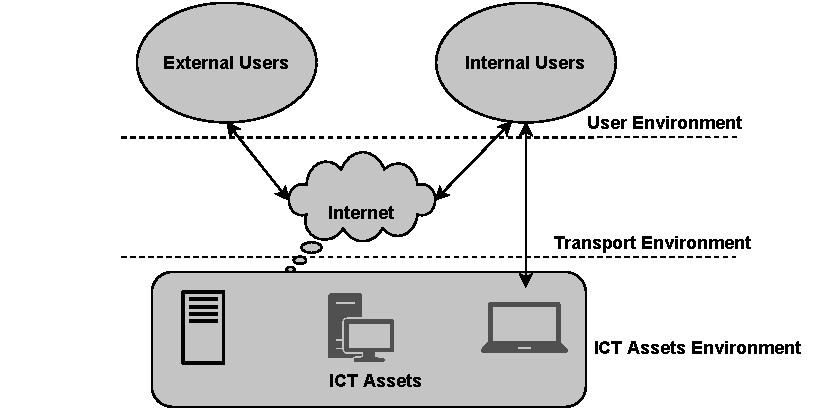
\includegraphics[width=\textwidth]{security-environment}
 	\caption{Security Environment.}\label{fig:security-environment}
 \end{figure}
 
The security environment consists of three distinguishable areas or environments,
each of which is subject to different types of threats and consequently needs different
security treatment:
\begin{itemize}
	\item The \textit{User Environment}
	\item The \textit{Transport Environment}
	\item The \textit{ICT Assets Environment}.
\end{itemize}
 
 Table {\ref{tab:security-model}} brings out the essence of the security model
 \begin{landscape}
 \begin{table}[ht]
 	\caption{Security Mode of e-Government.}\label{tab:security-model}
 	\begin{tabular}{p{5.5cm}p{5.5cm}p{5.5cm}}
 		\toprule
 		\textbf{Environment}                                                                    & \textbf{Management systems}                                                                              & \textbf{Management tools}                                                                                                                                                         \\ \midrule
 		{\bfseries User Environment\par}{$\bullet$ Internal users\par $\bullet$ External users} & {$\bullet$ Identity Management\par $\bullet$ Access Management\par $\bullet$ Interaction Management} & {$\bullet$ Passwords\par $\bullet$ Digital identity token\par $\bullet$ Access Control Lists (ACL)\par $\bullet$ PKI\par $\bullet$ Biometrics\par $\bullet$ e-government gateway} \\ \hline
 		
 		{\bfseries Transport Environment\par}{$\bullet$ Within LAN, WAN\par $\bullet$ Over the Internet} & {$\bullet$ Secure Communication System\par $\bullet$ Cryptographic Systems\par} & {$\bullet$ Government secure Intra-net\par $\bullet$ Virtual private networks\par $\bullet$ Government Secure Internet (GSI)\par $\bullet$ Encryption} \\ \hline
 		
 		 {\bfseries ICT Assets Environment\par}{$\bullet$ Tangible assets\par $\bullet$ Intangible assets} & {$\bullet$ Physical Security\par $\bullet$ Electronic Security\par} & {$\bullet$ Firewalls\par $\bullet$ Intrusion detection systems\par $\bullet$ Anti-virus systems\par $\bullet$ Disaster recovery site} \\ 
 		\bottomrule
 	\end{tabular}
 \end{table}
\end{landscape}
 
 From the security perspective, the e-government environment can be imagined to consist of three portions: 
 \begin{itemize}
 	\item the \textit{User environment}
 	\item the \textit{Transport environment} and
 	\item the \textit{ICT Assets environment}.
 \end{itemize} 
Users can be internal or external. Transport can be over private or public networks. ICT assets can be Tangible or Intangible.

\subsection{User Environment}
Security Management of user environment involves asking three basic questions of
individuals seeking to access the information system or to interact with it.
\begin{enumerate}
	\item \textit{Who are you?}
	\item \textit{What are you permitted to do with the system?}
	\item \textit{What are you accountable for in your interactions with the system?}
\end{enumerate}

 This is the objective of the three management systems shown in Table {\ref{tab:security-model}} -Identity Management Systems, Access Management Systems and Interaction Management Systems. 
 
 \subsubsection*{Identity Management Systems} 
 The objectives of an Identity Management System are:
 \begin{itemize}
 	\item To create unique \textit{digital identities} or credentials to all legal persons—citizens
 	and businesses—after establishing their existence and identifying them with
 	reference to name, date of birth, etc.
 	
 	\item To create and manage directories which link the digital identities with the real world identities and provide for their \textit{accessibility} to all other persons seeking to
 	communicate with them.
 	
 	\item  To create and manage ICT systems which ensure that the digital identities are \textit{secure}, i.\ e.\ they are not stolen, easily tampered with or ‘broken into'.
 	
	\item To \textit{revoke} the digital identity of a person when its confidentiality has been compromised or such identity is not otherwise required, by virtue of the death of such person or cessation\footnote{Put an end to an activity} in the role or office.
 \end{itemize}
 
 Examples of Identity Management Systems are:
\paragraph*{Username and password management system}

 A simple and `conventional' \textit{username and password} management system together with appropriate directory management services. The following
 guidelines are provided in this regard:
 
 \begin{enumerate}[label=(\alph*)]
 	\item Government agencies should \textit{clear-cut password policies} that prescribe things like the minimum password length, complexity of the password in terms of mandatory combination of alpha-numeric and special characters, life period of
 	a password that forces users to change the password, restriction on adopting the
 	same password time and again and procedures for revocation of password.
 	
 	\item It is advisable that the directory be maintained securely and centrally so that
 	it is available to all authorized users.
 	
 	\item Lightweight Directory Access Protocol (LDAP) compliance is preferable
 	when a very strong security is not required.
 	
 	\item Implement a fault-tolerant solution that provides $ 24 \times 7 $ availability of
 	directory services.
 	
 	\item Design and use a meta-data schema together with a taxonomy that prescribes
 	what information of the person is registered and in what uniform format and what
 	are the classes of users and their hierarchies. Omission in this regard could lead
 	to a serious confusion in the registration and retrieval processes as the
 	e-government systems scale up to a few thousand users.
 \end{enumerate}
 
 \paragraph*{Public Key Infrastructure}
 Public Key Infrastructure (PKI) is a more advanced system that not only
 contains an Identity Management System but also the features of the other two
 systems, viz.\ Access Management System and Interaction Management System.

 
 
 
 \subsubsection*{Access Management Systems}
 An Access Management System serves the following objectives:
 
 \begin{itemize}
 	\item It enables ICT systems to identify the user uniquely by matching the password, digital identity token or other device that carries the digital identity of the user with that registered in the system.
 	
 	\item It authorizes the user to perform only those tasks and transactions that are
 	predefined as per the privileges granted by the system administrator at the time
 	of registration or subsequently.
 	
 	\item It can maintain intelligence of users who try unauthorized access of tasks for
 	which they are not privileged. This would be available to the management for
 	review and remedy.
 \end{itemize}

\textit{Access Control Lists (ACLs)} and \textit{Advanced Access Control Lists} are industry
standards in this area.
 
 
 \subsubsection*{Interaction Management Systems}
 The objectives of interaction management are by far the most comprehensive and complex.
 They include assurance of the following principles of a comprehensive security, which are,
 in a way, the founding pillars of interaction management.
 
 \paragraph*{Authentication}
 Authentication or the assurance that the user is actually the person who s(he) claims to be.
 
 \paragraph*{Integrity} 
  Integrity or the assurance that the message or document sent or transaction effected\footnote{Settled securely and unconditionally} through an ICT system has not been tampered with, traveled from to destination safely and got stored therein securely.
  
  
  \paragraph*{Confidentiality}
  Confidentiality or the assurance that the content of the message or document sent
  or transaction effected has not been read by anyone else except the person to
  whom it has been sent.
  
  \paragraph*{ Non-repudiation}
  Non-repudiation or the assurance that the person who has transacted shall not
  repudiate the same at a later date.\\
  
  
  The above four axioms are fundamental to a secure digital environment and
  flourishing of e-government transactions. These are more significant for the e-government
  scenario because these four requisites are precisely needed for a whole gamut\footnote{A complete extent or range} of
  e-government transactions involving exchange of contracts, title deeds, issue of statutory
  certificates, financial transactions, filing of tax returns, approvals and sanctions accorded
  through a work-flow, etc. PKI is a mechanism that gives all the four assurances.
  
 \subsubsection*{Tools for User Management}
 \paragraph*{Username and Password system}
 Username and Password system is the conventional system of user management. It has
 several security issues. The user can compromise the password. The password can be
 hacked. The password can be transferred. It does not assure that the person keying in the
 password is the real-world person to whom it was assigned.
 
 \paragraph*{Digital identity token}
 A digital identity token is a popularly used device to overcome some
 shortcomings of a simple password. It is a photo ID card that also has the password
 embedded in it either magnetically or as a chip. It serves the dual purpose of controlling
 the physical access to the work premises and of controlling access to the ICT systems that
 the user is authorized to access. It is quite suitable for employees in corporate work
 environments. The digital identity token is not completely foolproof or transfer-proof
 because it depends on human intervention at the entry point through verification of the
 photo ID with the person's face.
 
 \paragraph*{Biometric device}
 A biometric device seeks to overcome the deficiencies of a token by using the
 physical features of a person, such as the fingerprint or iris to establish identity uniquely.
 These features are captured at the time of registration, converted into a code using certain
 algorithms and stored for comparison at the time of authentication. 
 
 \paragraph*{Public Key Infrastructure (PKI)}
 Public Key Infrastructure (PKI) is a technology that is based on the theory of cryptography or converting an intelligible text or digital content into a form that can be
 decrypted and read by the user or person to whom it is sent. PKI basically uses the
 concepts of \textit{Digital Signature Certificate}, \textit{Asymmetric Key Pair}, \textit{Public Key}, \textit{Private Key}, Digital Signature and Encryption. 
 
 \subparagraph*{Digital signature certificate}
 A digital signature certificate is a document issued by Certification Authority (CA), legally clothed with powers to do so, to a person, creating the digital
 identity of that person after satisfying that the person truly is who s(he)
 claims to be. The CA may employ a number of Registration Authorities (RAs) for
 conducting such verification and front ending the process of issuing digital
 signature certificates. The digital signature certificate also contains the \textit{public key}
 of the person, besides details like name, address, and date of
 validity of the certificate. The CA can revoke a digital signature certificate in case
 it is no longer required or the user violates the conditions of the certificate, such
 as compromising the \textit{private keys}.
 
 \subparagraph*{Asymmetric key pair}
 An asymmetric key pair is a set of two complimentary keys or codes, generated
 using an algorithm such that:
 \begin{enumerate}[label=(\alph*)]
 	\item  a text, document or message encrypted using one key can be decrypted only by the other key, and
 	\item it is not possible to derive one key from the other.
 \end{enumerate}

\subparagraph*{Public key}
A public key is that part of an asymmetric key pair that is displayed or published
for information and usage by public. It is a part of the PKI directory. The public key of a person is used by others to send an encrypted message
to that person. The public key of a person is also used by the recipient of a
message or document in verifying the digital signature of a person attached to a
message or document.


\subparagraph*{Private key}
A private key conversely is the second of the key pair that is to be retained and
stored confidentially by the holder of the digital certificate. The private key is
used by a person.
\begin{enumerate}[label=(\alph*)]
	\item to decrypt messages sent by others (using his or her public key), and
	\item to digitally sign a message or document.\\
\end{enumerate}
 
PKI, if implemented as part of a comprehensive security policy, can meet the
requirements of authentication, integrity, confidentiality and non-repudiation.

Setting up of PKI in a country involves the following steps:

\begin{steps}
	\item Enacting legislation required to give legal status to electronic transactions
	conducted in conjunction with PKI.
	
	\item Selection of agencies in the public and private sectors, which can be licensed to
	set up the required infrastructure and act as CAs, after conducting an audit of their
	capabilities and track record.
	
	\item Promoting the use of PKI for e-government, by taking up specific initiatives in the areas of taxation, customs clearances, land titles and such high-value, high-stake areas.
	
	\item Notifying the designated official or group within the agencies piloting the PKI
	within e-government as RAs.
	
	\item Perhaps, as may be required initially, to subsidize the cost of digital certificates
	to promote the concept, as otherwise, the cost of a certificate could be prohibitive
	at low volumes.
\end{steps}

Example of PKI: \textit{RSA Security}.

 \subsection{Transport Environment}
 Transport Environment includes all the space between the users internal and external and the ICT assets of the e-government system. The need for maintaining the authenticity, integrity and confidentiality of the information is as important here from the security point of view as in the other two environments. Transport Environment is also one over which the administrators of the e-government systems do not have a total control—physical or electronic.

 Transport Environment consists of the LANs, WANs, wireless and RF networks, satellite-based networks (VSAT) besides the Internet, which is a critical component the transport infrastructure. All the networks except the Internet can be secured through appropriate means, within the control of the administrators. There are \textit{three} popular ways of tackling the security issues arising out of the use of Internet:
 
 \begin{itemize}
 	\item Creating a Virtual Private Network (VPN) in the public domain
 	
 	\item Installing firewalls at each interface point between the Internet and the agency networks and
 	
 	\item Encrypting the data communicated over the Internet.
 \end{itemize}

\subsubsection*{Virtual Private Network (VPN)}
VPN is a secure network over an insecure network.
VPN technology involves creation of a secure, ‘private’ network—or a tunnel—in a public network to provide secure communications. VPNs provide confidentiality by
encrypting data sent over it. They provide integrity by using \textit{checksums} to ensure packets are not corrupt. VPNs verify the identity of the sender before establishing the connection with the agency intranet. They also have features that support access management and non-repudiation.

The benefits of VPN include cost savings, security that is better than in a purely
Internet-based communication channel and enable remote access of ICT resources without a dedicated connection.

VPN technology involves three components — a \textit{VPN client} software, a \textit{VPN gateway}
at the entry point of the agency or enterprise and a \textit{VPN management application} that
ensures the features of PKI are integrated. IPSec (Internet Protocol Security) is the protocol most commonly used in creating VPNs. At the client end, IPSec encrypts the data packets,
encapsulates them in an ESP (Encapsulating Security Payload), which is then enclosed in
an IP packet and transported. The process of ‘unpacketing’ and decrypting happens at the VPN gateway.

VPN is not an unmixed blessing. There are issues such as the following:

\begin{enumerate}
	\item The payload of security in encryption and decryption is heavy
	
	\item There are performance and QoS issues
	
	\item Prone to Denial of Service Attacks
	
	\item Scalability issues
	
	\item Management issues, especially those relating to client side
\end{enumerate}

\paragraph*{VPNs for e-Government}
\emph{e-government often involves establishing a secure connectivity between the HQs of various agencies and its remote field agencies, to support enterprise-wide applications. Establishing dedicated networks involves expense and time much beyond permissible limits. In such circumstances, VPN can be evaluated as a viable option.}

 \subsection{ICT Assets Environment}
 ICT assets are by far the most valuable and sensitive from the point of the enterprise. The hardware, the software, databases and knowledge is held centrally in the conventional EDP winds or in data centers. As shown in Table {\ref{tab:security-model}}, two broad categories of security treatments
 are required here—the \textit{physical security} and \textit{electronic security}.
 
 \subsubsection{Physical Security}
 \textit{Physical security} involves steps that guard against physical damage or loss, These steps include:
 
\begin{enumerate}
	\item Aggregation of the core ICT assets in highly guarded data centers, with restricted entry through biometric-controlled doors.
	
	\item Provision of dust-proof air-conditioned environment in the data centers,
	preferably built to industry standards, with raised floor, special cabling for power and communications, fire protection systems, alarms and closed-circuit TV
	monitoring of the premises, etc.
	
	\item Discouraging or prohibiting the use of USBs that are likely to infect the
	systems with viruses.
	
	\item Prohibiting the use of the assets of the system for personal e-mail and browsing.
	
	\item Providing fail-over and redundant systems to ensure $ 24 \times 7 $ availability and eliminating single points of failure.
	
	\item Rigorous and automated systems of backup and archival.
	
	\item Maintenance of audit logs and their review.
	
	\item Deployment of biometric-controlled access to workstations and applications.
	
	\item Provision of high quality UPS systems for guarding against power fluctuations and outages.
	
	\item Above all, mirroring of the core data and applications in a remote Disaster
	Management site.
\end{enumerate}
 
\subsubsection{Electronic Security}
 \textit{Electronic security} involves placing controls at all the digital entry and exit points to monitor the digital traffic that enters and goes out of the enterprise. The electronic security tools broadly fall under three categories:
 \begin{multicols}{2}
	\begin{itemize}
		\item Anti-virus systems
		\item Intruder detection systems
		\item Firewalls
	\end{itemize} 
 \end{multicols}

 \paragraph{Anti-virus systems}
 A computer virus is a malicious software program that is capable of attaching itself to executable files, data, hard disks or to removable disks and can execute itself repeatedly, replicate itself several times or propagate itself over networks without the knowledge or permission of the user. Such repeated execution, replication or propagation may have the dangerous effects, such as the following, in increasing degree of damage to the host system.
 
 \begin{itemize}
 	\item Occupying valuable disk space
 	\item Slowing down of the system due to excessive consumption of the memory
 	capacity
 	
 	\item Slowing down or clogging of networks
 	
 	\item Corruption of data residing on hard disks and other media
 	
 	\item Corruption and the consequent dysfunction of the application programs
 	
 	\item Infecting the other computer systems that the user’s system communicates with.
 \end{itemize}

Virus programs are written and propagated by their authors purely with malicious
intentions of causing inconvenience or damage to the targeted users or to the community
of computer users at large. The virus programs are also called \textit{malware}. Virus programs are
the instruments of cyber-terrorism and pose an unknown but serious threat to the security
of all computer systems. The computer community has to guard itself of the dangers posed
by the virus menace\footnote{threat} appropriately to protect the ICT assets and to provide
information and services in a reliable manner to the customers and to continue internal
operations without a break.

The other broad categories of malware programs are \textit{worms} and \textit{Trojan horses.}

\textit{Worms} are parasitic computer programs that replicate themselves without infecting other
computer files, either on the user’s computer or in the other systems to which the user is
connected over a network. 

A \textit{Trojan horse} is a computer program that pretends to be a
harmless program but actually executes certain actions that the user does not expect to do.
It is not a virus in the strict sense as it does not replicate itself.

\paragraph*{Types of viruses}
Computer viruses are as variant, stubborn and painful as their biological counterparts. It is
essential to know these broad categories to be wary of the possible consequences and
take preventive security measures.

\subparagraph*{Boot sector virus}
 \textit{Boot Sector Infector (BSI)} is a virus that gets access to and
resides in the boot sector or the area of the computer (usually on the hard disk) where the initial programs required to start a computer are stored. Whenever the
computer tries to read the boot program, the virus gets into the memory and executes itself
to gain control over all the computer operations. It can infect all the files and also
propagate over the network fast. It is quite a nasty species as it poses immense problems
to get rid of.

\subparagraph*{Macro virus}
A malicious program written in macro language (a language used to conduct repetitive tasks in a computer product, e.g. MS Word or Excel) that attaches
itself usually to Word documents and does its damage whenever the document is Opened
It also spreads to other document files. It can be highly annoying.

\subparagraph*{Encrypted virus}
A virus that propagates in an encrypted manner to escape
detection by the anti-virus software. The virus also carries its own decrypting algorithm. 
Each time it decrypts itself, it produces a different code that can cause the intended damage
to the system. By virtue of the unpredictable sequence of the decrypted code, the encrypted
virus escapes detection. Variants of the encrypted virus are the:
\begin{itemize}
	\item \textit{Polymorphic virus }(which
	creates varied versions of itself, but containing its original potential to damage),
	\item \textit{Mutating virus} (which mutates or changes as it progresses through its course in the host system),
	\item \textit{Self-encrypting virus} (which encrypts its signature code differently each time it infects),
	\item \textit{Self-garbling virus} (which garbles its code when it is in transmission, but ‘degarbles’ itself when the host program has infected runs) and
	\item \textit{Stealth virus} (which intercepts the disk
	access requests made by the anti-virus programs and feeds them a clean image of the
	infected file to indicate the file size as it was before infection).
\end{itemize}
All these categories of viruses are intended to deceive the anti-virus software, conceal themselves in different ways, escape detection and proliferate\footnote{Grow rapidly}.

\subparagraph*{Anti-antivirus viruses}
These are virus programs that infect and disable specific
anti-virus programs installed on a system and thereby continue their damage.

 \subparagraph*{Antivirus virus}
 These are viruses that specifically look for and remove other viruses.
 
 
\paragraph*{Relevance of anti-virus software to e-government}
Securing e-government systems from viruses is extremely important for the following
reasons:
 \begin{itemize}
 	\item \textit{Availability} of e-services on a $ 24 \times 7 $ basis is a requisite. e-government systems 
 	cannot be shut down for disinfection as it would adversely affect the reliability.
 	\item \textit{Trust and confidence} of the citizens would be shattered if the valuable
 	transactions recorded by them in e-government systems get corrupted or obliterated\footnote{Reduced to nothingness} due to virus attack.
 	\item Several \textit{sensitive} functions would be seriously affected in the event of a virus
 	attack.
 	\item e-Government systems have special \textit{vulnerability} from the point of view attacks by authors of viruses.
 \end{itemize}

\paragraph*{Anti-virus techniques}

\subparagraph*{Prevention}
 Agencies and enterprises should have rigid and clear virus prevention policy as part of their overall security policy. It should lay down severe restrictions on the usage of USBs, downloading pirated games or games and programs from untrusted sites and other potentially virus-carrier programs, send timely alerts to all users against opening e-mail suspected to carry virus, and do regular scanning of all systems and so on.


 \subparagraph*{Protection} 
Defense in depth and an integrated
solution are recommended practices in virus protection. The defense in depth method involves appropriate steps and solutions at three levels, namely, the \textit{user level}, the \textit{backend systems level} and \textit{perimeter level}. 

\subsubsection{Intrusion Detection Systems}
Intrusion Detection Systems (IDS) are automated monitoring systems that watch for
abnormal, unauthorized or malicious activities. The role of IDS is to watch the traffic
patterns, analyze traffic content, review the firewall log files and monitor user account
activity. IDS can warn system administrators when an attack or intrusion is taking place.

Depending on the sophistication of the IDS, it can be configured to repel attacks on the fly
or track down the origin of the attack. It is not strictly required to protect the network from
Internet-based attacks, but it does provide a more extensive and automated monitoring
system. Repeated unsuccessful attempts to access the systems, accessing the systems
apparently by registered users but at unexpected hours or from different locations,
unprecedented high volume of traffic coming from a particular source, etc.\ are enough
reasons for the IDS to suspect a security breach and to alert the administrators.

\subsubsection{Firewalls}
Firewall is a computer system or a group of systems hardware and software that an access control policy between two separate networks, such as between two LANs or two WANs or a LAN and a WAN or most usually between a LAN/WAN and the Internet. The key feature about a firewall is that is only a mechanism to enforce the access control policy of the agency. The prerequisite for the successful deployment of a firewall, therefore, is the design and promulgation of an enterprise security policy. Firewall serves the basic purpose of making it nearly impossible for unauthorized users to access the ICT assets (situated `behind' the firewall) while permitting the authorized users to access the same effortlessly.

Firewalls typically adopt the following techniques for the ‘inspection’ required for
implementing the security regime. An understanding of these techniques enables
e-government managers to better manage the security policy.

\paragraph*{Packet filtering}
The firewall filters the IP packets with reference to the do’s and
don’ts or security rules prescribed by the organization. It validates the intelligence
it gathers from each packet against such rules.

\paragraph*{Network Address Translation (NAT)}
Firewalls also translate or replace the
internal or private IP numbers assigned to systems within the network with its
own public IP address so that the individual systems within the LAN of the
enterprise are not visible to the outside world and are more secure to that extent.

\paragraph*{Application proxy or proxy server}
A firewall can also act as a proxy of the
systems within the network, when such systems want to interact with the outside
world for such services as e-mail, Internet access, file transfer, etc. A proxy server
acts as a buffer between the internal workstations and the Internet.

\paragraph*{Logging and monitoring}
Firewalls have features that keep a record of the
events that happen within its purview. All exceptional or abnormal events are so
logged, for review by the security administrators. In the event of a high risk anticipated at the firewall, it is programmed to send appropriate alerts to the
security administrators for prompt remedial action. For instance, when the
firewall suspects a ‘sniffing’ or pre-attack surveillance by an outsider, it sends such an alert.

\paragraph*{Content filtering}
Firewalls use the technique of content filtering to block
objectionable sites being accessed by the users or messages containing predefined
objectionable or obscene words being sent out of the system or received into it.

\paragraph{Types of Firewalls}
Firewalls are basically of two types: \textit{hardware firewalls} and \textit{software firewalls}.

\subparagraph{Hardware Firewalls}
These are security appliances that contain the hardware and
software bundled into one. The firewall software is preloaded into the appropriately sized
hardware and configured for optimum performance with the result that the setup is quite
quick. Hardware firewalls are the preferred option when an organization wants to put in
place a security system quickly following a serious attack. Hardware firewalls tend to be
more expensive and less flexible as compared to software firewalls.

\subparagraph{Software firewalls}
These are software packages that need to be installed on the
existing hardware of the enterprise or hardware procured separately for the purpose. Due
to the availability of a wide range of software firewall products in the market, this would
be a preferred solution when the security needs of the agency are specific. Software
firewalls are less expensive, but require more time for installation and user training. There
are also personal firewalls for free download, which are suitable for standalone PCs.



\section{e-Government Security Architecture}
 Security Architecture is a high level document that directs and guides the security  efforts of individual e-Government initiatives and projects setting out the security objectives and goals, prescribing the standards to be achieved and indicating the procedures and processes that need to be followed by all the players participating in e-government, users, citizens, businesses, e-government partners, operators and service providers.
 
 The goals of the security architecture are to:
 \begin{itemize}
 	\item Create the necessary levels of confidence and trust among the stakeholders-citizens, businesses and government users.
 	\item Enforce global standards of security practice and implementation in e-Government.
 	\item Create and enforce digital identities including registration and enrollment as a means of accessing electronic government services.
 	\item Strengthen the four pillars of security i.\ e.\ \textit{authentication}, \textit{integrity}, \textit{confidentiality} and \textit{non-repudiation}.
 	\item Enhance the security awareness among the users through dissemination of a set of security guidelines.
 	\item Promote the development of operational schemes called security policies by individual government agencies.
 \end{itemize} 

 Security architecture seeks to achieve the above objectives by addressing the regulatory, technological and managerial issues arising out of the security needs and requirements of
 \begin{multicols}{2}
	\begin{itemize}
		\item user environment
		\item transport environment
		\item ICT assets environment.
	\end{itemize} 
 \end{multicols}


The security architecture, usually accompanied by a set of security guidelines, contains the following:
\begin{itemize}
	\item A description of the security environment consisting of the three portions mentioned above and what the e-government assets are the need to be secured and what the perceived security threats are.
	
	\item A description of the security requirements in functional and technical terms.
\end{itemize}

Any national or state government, intending to take up an e-government initiative seriously, should design an appropriate Security Architecture and Framework as a first step. This sets up the security vision in clear terms.

The formulation of a Security Architecture and Framework has to be quickly followed by three more initiatives:

\begin{itemize}
	\item Providing a \textit{statutory basis} for the e-government security architecture and mandating the security requirements on agencies that are partners in e-Government.
	\item Defining \textit{security standards} to be followed.
	\item Encouraging individual agencies in the public and private sectors to design appropriate \textit{security policies} that give a concrete shape to the manner of implementing the architecture in specific relation to the particular agency or enterprise.
\end{itemize}
 
 \section{Security Standards}
 The standards for information security was set up by the \textit{British Standard BS 7799}, which on account of its immense popularity was adopted by the ISO as \textit{IS0 17799}. There is also a sequel \textit{BS 7799-2} that prescribes the specification for Information Security Management.
 
 The versions of these security standards are \textit{ISO/IEC 17799}, which is the Code of practice for Information Security Management, and \textit{BS7799-2:2002} which gives the Specification for Information Security Management.
 
\textit{ISO/IEC 1799} is a standard that sets out the requirements for an Information Security Management. It helps identify, manage and minimize the range of threats to which information is regularly subjected. It defines 127 security controls structured under 10 major headings to enable the IS managers to identify the particular safeguards that are appropriate to their particular business or specific area of responsibility. 

\textit{BS7799-2:2002} tells us how to apply \textit{ISO/IEC} 17799 and how to build, operate, maintain and improve an ISMS.

The 10 major security areas identified by \textit{ISO/IEC 1799} and the ISMS methodology of implementing the security are mentioned briefly below, as they are central to an e-Government security policy.

\subsection[ISO/IEC 17799]{Ten Controls Prescribed By ISO/IEC 17799}
\begin{enumerate}
	\item \textit{Security policy}: Provides management direction and support for information security.
	
	\item \textit{Personal security}: Reduces the risks of human error, theft, fraud or misuse of facilities.
	
	\item \textit{Access control}: Secures management of access to information.
	
	\item \textit{Compliance}: Avoids breaches of any criminal and civil law, statutory, regulatory or contractual obligations, and any security requirement.
	
	\item \textit{Systems development and maintenance}: Ensures that security is built into information systems at the design and development stage.
	
	\item \textit{Communications and operations management}: Ensures the correct and secure operation of information communication and processing facilities.
	
	\item \textit{Organization of assets and resources}: Helps manage information security within the organization.
	
	\item \textit{Asset classification and control}: Helps identify assets and protect them appropriately.
	
	\item \textit{Physical and environmental security}: Prevents unauthorized access, damage and interference to business premises and information.
	
	\item \textit{Business continuity management}: Avoids interruptions to business activities and protects critical business processes from the effects of major failures or disasters.
\end{enumerate}

We can see that
\begin{itemize}
	\item the first five controls relate to the user environment
	\item the sixth one to transport environment and
	\item the remaining four to the ICT assets environment.
\end{itemize}
 
\subsection[ISMS]{Information Security Management System (ISMS)}
The information Security Management System (ISMS), also called Information Security Policy, is a document prepared by a government or an agency and addresses the following questions:

\begin{itemize}
 \item Why is information security important in the context of the e-government program or initiative?
 
 \item What are the threats perceived to be important? What are the possible attacks? What is the level of risk that the agency can accept or tolerate?
 
 \item What are the environments that we want to protect? In other words, who are the users, what are the communication channels, and what are the ICT assets that we want to protect? List, identify and classify them.
 
 \item What are the roles and privileges that we want to give to the users of various categories? Who is allowed to do what? What is the policy of the enterprise for e-mail, chat, web access, system administration, development and maintenance?
 
 \item How do we want to treat or manage the risks identified with the controls selected? In other words, what tools do we intend using for treatment of risks?
 
 \item What are the organizational arrangement that ensure management of the security policy and its continuous review and audit?
\end{itemize}

The ISMS of Information Security Policy is a working document that guides, instructs and canalizes the actions and efforts of all users of the ICT systems. Figure {\ref{fig:pdca-model}}, adopted from the Standard, defines a PDCA or Plan-Do-Check-Act cycle for management of the security.

%%%%%%%%%%%%%%%%%%%%%%%%%
%						%
%		Figure	  	 	%
%						%
%%%%%%%%%%%%%%%%%%%%%%%%%
\begin{figure}[hpb]
	\centering
	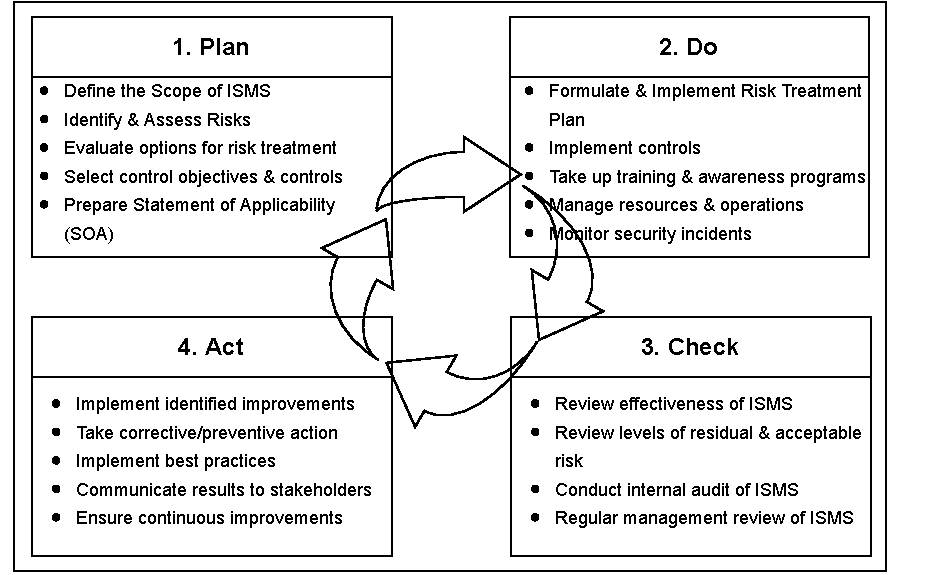
\includegraphics[width=0.8\textwidth]{pdca-model}
	\caption{The PDCA Model of Security Management.}\label{fig:pdca-model}
\end{figure}

 
Information Security is quite critical to the success of e-Government. We need a comprehensive security approach that spans across the user, transport and ICT assets environments. Publication of an e-government security architecture and preparation of an Information Security Management System, in conformity with the international standards are the most desirable practices.




  % ch-5: Security for e-Government
\chapter{Managing e-Government}
Management of e-Government implementation involves the following:
\begin{multicols}{3}
	\begin{itemize}
		\item people
		\item process
		\item technology
		\item finance and
		\item partnerships
	\end{itemize}
\end{multicols}


\section*{Managing People}
e-Government has to be designed, developed, delivered and used by people --- people within government agencies, people outside the government in organizations that government would have to partner, citizens and business people. People management involves the following:

\begin{multicols}{2}
	\begin{itemize}
		\item Awareness building
		\item Education
		\item Training
		\item Coordination
		\item Team building
		\item Development of leadership qualities
	\end{itemize}
\end{multicols}


\section*{Managing Process}
\begin{itemize}
	\item \textbf{Service definition}: e-Government is about being service-centric.
	\item \textbf{BPR (Business Process Re-engineering)}
	\item \textbf{Legal process reform}
	\item \textbf{Delivery channel reform}
\end{itemize}


\section*{Managing Technology}
\begin{itemize}
	\item \textbf{Design and development of architectures}
	\item \textbf{Prescription of standards}
	\item \textbf{Security}
	\item \textbf{Procurement}
\end{itemize}

\section*{Financing e-Government Projects}
We need experts who can find innovative methods of financing e-government projects.

\section*{Managing Partnerships}
\begin{itemize}
	\item \textbf{Designing suitable partnership models}
	\item \textbf{Crafting the contracts}
	\item \textbf{Steering the partnerships}
\end{itemize}

 \section{Approaches to Management of e-Government Systems}
There are different ways in which management for e-government can be understood. Three possible approaches to e-government responsibilities (see Figure \ref{fig:e-government-approaches}):

%-----------------------------------
%		figure%
%-----------------------------------

\begin{figure}[tph]
	\centering
	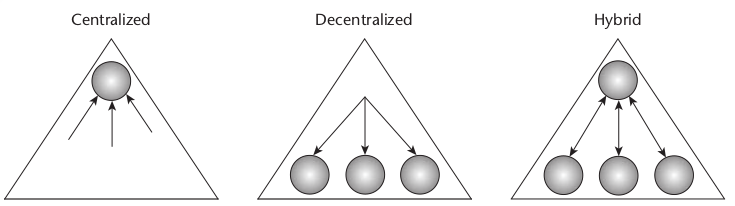
\includegraphics[width=0.9\textwidth]{e-government-approaches}
	\caption{Different approaches to e-government systems responsibilities}
	\label{fig:e-government-approaches}
\end{figure}
\begin{enumerate}
	\item \textbf{Centralized}: Decisions are taken at the most senior or central level.
	
	\item \textbf{Decentralized}: Decisions are taken at some level lower than the most senior; typically by individual work units within the organization or even by individual staff. The latter may also be referred to as end-user computing, where the individuals within the public sector who make use of outputs from e-government systems (the internal
	end users) are also those who operate and/or develop and/or manage those systems.
	
	\item \textbf{Hybrid}: Decisions are taken at both senior and lower levels, either separately or in an	integrated manner. This approach is called federal or federated in some governments.
\end{enumerate}

\subsection[Centralized Approach]{Centralized Approach to e-Government}
Some examples can be given of what a centralized approach to e-government would
mean. In terms of computing and data management architecture, a centralized computing architecture would be one which involves a large central computer with dumb terminals or network computers attached. That represents an internal view of architecture. An external view sees centralized data architecture in terms of portals: single central web locations through which all data is routed to users. 

Under a centralized approach, e-government systems are typically developed by a team from the central IT unit, or by external contractors under central IT unit control. The content and timing of individual projects can be drawn from any e-government strategy that has been developed. That strategy could also be used to guide procurement, where organization-wide
standards would be set for hardware, software and telecommunications equipment. Typically, a central group is responsible for setting standards, arranging contracts with suppliers, policing standards, and giving final approval on all IT purchase requests. Purchases of IT and IT budgets are routed through a central control point.

In a centralized approach, training is planned and prioritized organization-wide to fit in with e-government plans. Like technical support, it may be delivered by external providers or by specialist staff from the central IT unit. 

\subsubsection{Benefits of a Centralized Approach}

\paragraph*{Achievement of scale economies}
Centralized approaches allow most activities to be undertaken more cheaply per unit. Items purchased externally — computers, software packages, consumables, staff training, systems development, consulting, and so on — can be decided upon once and then bought in greater bulk.
Activities undertaken internally — from system development to implementation
and maintenance, and management of all these processes — cover a greater number of staff.

\paragraph*{Avoidance of duplication}
One main intention of centralized approaches is to have a single version of any particular e-government system for the whole organization, and to store any item of data once and only once. As a result, there is no wasted effort, no wasted storage
capacity, and no inconsistency of data. For example, only one accounting application needs to be developed for the whole agency. Similarly, if dealing with a set of external clients (such as businesses), each client’s name and details are captured once for use on a single, shared database. If these details change or if the required data structure changes, only one set of amendments needs to be made. The database represents the single authoritative source of digital information in the organization. This saves money, and can also improve data quality.


\paragraph*{Sharing resources}
A well-planned centralized system holds data used across the organization in one place, allowing all staff to access it. This makes it cheaper, faster and easier to undertake organization wide activities. Central planning and operation also allows compatible technology and skills to be introduced. Exchange of hardware, software and staff between
organizational systems and units therefore becomes much easier and less costly.



\subsubsection{Disadvantages of Centralized Approaches}

\paragraph*{Heavy time consumption}
Centralized decisions and actions can be
more time-consuming than for a decentralized approach because of: 
\begin{itemize}
	\item the additional time it takes for information to flow up the organization as an input to centralized decisions;
	\item the additional time it takes to collate information from a variety of different decentralized locations as an input to centralized decisions; and 
	\item the additional time it takes for implementation information to flow down the organization.
\end{itemize}


\paragraph*{Limited ability to meet user needs}
Centralized approaches necessarily mean that priority goes to those e-government systems which are seen as important by some select and centralized staff group. The priorities of the periphery – both individuals and individual work units inside government, as well as clients outside government may not be addressed.


\paragraph*{Inflexibility}
The greater the amount of central planning that has gone into an e-government system decision, and the longer that decision is therefore intended to provide guidance for the organization, the less flexibility it offers the organization to cope with differences between local units, or with internal or external changes.


\subsection[Decentralized Approach]{Decentralized Approach to e-Government}
Examples of a decentralized approach to managing e-government systems responsibilities
can be provided. In terms of computing and
data management architecture, a truly decentralized computing architecture would be one
that involves standalone computers or, possibly, a peer-to-peer network. Decentralized
approaches are commonly associated with the
spread of personal computers throughout an
organization. An external view would see
multiple websites and other routes through
which data could be accessed.

Under a fully decentralized approach,
e-government systems would be developed
within organizational work groups, focused
on their requirements, or even by individual
end users. Decentralized procurement means
that individuals or groups select and procure whichever technology best suits their
particular needs. Similarly, a decentralized
approach to training means that individuals
or small groups plan their own training
needs. It is likely that training takes place
on the job or through informal coaching of
one staff member by another.

\subsubsection{Benefits of Decentralized Approach}

\paragraph*{Greater fit between systems and local needs}

The closer the proximity of user and developer, the less the communication gap and
the more likely it is that the developed
system meets the users’ real needs.


\paragraph*{Faster system development}
The less the organizational distance between
system user and system developer, the faster
development of that system is likely to be.


\paragraph*{Perceived lower costs}
Decentralized approaches present lower costs than centralized approaches in certain areas. This is thanks to:
\begin{itemize}
	\item faster development, 
	\item less miscommunication, 
	\item greater fit to local needs through smaller design–reality gaps, 
	\item the greater emphasis on smaller computers, 
	\item the greater emphasis on buying software packages rather than developing software in-house, and so on.
\end{itemize}


\subsubsection{Disadvantages of Decentralized Approach}
\paragraph*{Barriers to sharing data}

Decentralized approaches can create e-government systems in different work units that are mutually incompatible.

\paragraph*{Barriers to sharing other resources, including human resources}
There may also be an inability to share
other resources if work units are allowed to
set up their own separate e-government systems. It may be hard to exchange hardware
and software. Perhaps more importantly,
each individual system requires a unique set
of skills for system development, implementation and operation. This makes it more
difficult for staff to move between different
e-government systems.


\paragraph*{Duplication of effort}
Decentralized approaches also tend to be very costly because units will often duplicate what others are doing.

Duplication covers analysis, design and implementation of e-government systems; gathering and administration of data; and system operation,
support and maintenance.

This imposes extra costs in gathering,
maintaining and updating data.

\paragraph*{Lack of learning and control}
In addition to the extra direct costs that
duplication imposes, there is an indirect
cost of lost learning opportunities and limited
cross-fertilization of ideas.



\subsection[Hybrid Approach]{Hybrid Approach to e-Government}
Both the centralized and
the decentralized approach to managing
e-government can provide benefits for public
organizations. Yet, at the same time, such
approaches can be hard or impossible to
implement, and can produce serious disadvantages for the organization.


What is the way out of this quandary?

One way forward is the adoption of a hybrid approach that attempts to reconcile the push of the centralized approach with the pull of the decentralized approach.



A hybrid approach to e-government can be feasible and
provide distinct benefits. A decentralized approach may be most economic for public
organizations, because it saves on overt input
costs. A centralized approach may be most efficient, because it avoids waste and duplication.
But a successful hybrid approach may be most
effective because it can simultaneously provide:

\begin{itemize}
	\item the control necessary to share key resources
	(including data), to avoid duplication, and
	to achieve economies of scale; and
	\item the freedom necessary to meet user
	needs, and to overcome blocks to IT
	usage and system development.
\end{itemize}



\subsubsection*{Examples}

\paragraph*{Computing and Data management architecture}
The most common hybrid computing architecture is the client/server model, in which computing power is divided between the central servers and the local client workstations. This architecture has now been adopted by vast numbers of public sector organizations worldwide.


A similar hybrid approach to portals
creates a single main portal which merely
links through to an existing set of sub-portals.


\paragraph*{Systems development}
A hybrid approach to systems development can involve a division of responsibilities; for example, defining certain types
of e-government system as suitable for
central development, and others as suitable
for decentralized/end-user development.

\paragraph*{Procurement}
Standards for procurement bring many
immediate and obvious benefits to public
agencies.

%--------------------------------end of section--------------------------
\section{e-Government Strategy}
An e-government strategy is a plan for e-government systems and their supporting
infrastructure which maximizes the ability of management to achieve organizational objectives. Increasing numbers of public agencies are developing an e-government
strategy.

\subsection*{Strategic Planning}
A set of core questions about e-government strategy for public agencies are:


\subsubsection*{Why?}
Why are increasing numbers of public agencies trying to develop an e-government strategy?

Following could be the explanations.
\begin{itemize}
	\item The fad/`me too’ factor of copying current trends or copying appearances in
	other organizations.
	\item The desire of some senior officials to wrest control of e-government from technical staff and/or individual departments.
	\item The desire for the kudos\footnote{An expression of approval and commendation} and resources associated with a major organizational
	initiative.
	\item The demand for such strategies from central government agencies.
\end{itemize}

In addition, the growth of e-government strategies in the public sector is
impelled by the potential benefits that a strategy can bring. 

Some of these are political, such as:
\begin{itemize}
	\item providing senior management control over organizational systems, 
	\item accessing central funds that are only	available on production of a strategy, and 
	\item avoiding public reprimands and penalties where strategies are demanded by higher level bodies.
\end{itemize}

An e-government strategy is also seen as
a key mechanism to produce centralized approach benefits


Finally, 
\begin{itemize}
	\item a successful strategy can develop
	senior management understanding that
	e-government systems are information
	systems not just IT.
	
	\item It permits a fundamental
	review of the organization’s use of information and technology, leading to a comprehensive understanding of information
	systems requirements. 
	
	\item It also provides a detailed plan of action on e-government for 	the organization.
\end{itemize}



\subsubsection*{What?}
Like any strategic plan, an e-government
strategy seeks to answer three questions,
illustrated in Figure \ref{fig:overview-of-strategic-planning}:
\begin{figure}[tph]
	\centering
	
\includegraphics[width=0.8\textwidth]{overview-of-strategic-planning}
	\caption{Overview of strategic planning}
	\label{fig:overview-of-strategic-planning}
\end{figure}

\begin{itemize}
	\item \textbf{Where are we now?} (i.\ e.\. how are systems working now, and what external factors affect them).
	
	\item \textbf{Where do we want to get to?} (i.\ e.\ in the future, how should the organization’s e-government systems be or work differently from at present).
	
	\item \textbf{How do we get there? }(i.\ e.\ what actions need to be undertaken to achieve the	outcome identified in answering the second question).
\end{itemize}


\subsubsection*{When?}
In simple terms, the answer is: ‘You undertake e-government strategy when the time
is right’.

In other cases, we undertake e-government strategy when:
\begin{itemize}
	 \item e-government systems being created without consideration for overall organizational objectives;
	\item outdated systems still in use due to inability to plan alternatives;
	\item data that cannot be shared between different e-government systems because
	there are no organization-wide standards;
	\item IT being seen as the end rather than the means; in other words, when
	e-government is seen as an end in itself;
	\item no clear locus of responsibility for dealing with these problems;
	\item comparative organizations have a strategy.
\end{itemize}

\subsection{Steps of e-Government Strategic Planning}
eGovernment strategic planning is typically conceived as a series of steps that are
undertaken systematically over a period of a few weeks or a few months. These steps are
summarized in Figure \ref{fig:steps-e-gov-planning}. Once completed, they produce a framework for organizational action that can endure for a number of years.

\begin{steps}
	\item Create e-government planning structures/roles
	\item 
	\begin{enumerate}[label=\alph*.]
		\item Audit information	systems
		\item Get guidance from	organizational strategy
	\end{enumerate}
	\item Set e-government objectives and principles
	\item 
	\begin{enumerate}[label=\alph*.]
		\item Determine e-government systems architecture
		\item Determine e-government organizational architecture
	\end{enumerate}
	
	\item Disseminate and plan e-government actions
	\item Manage, evolve and review e-government strategy
	
\end{steps}

\begin{figure}[hpt]
	\centering
	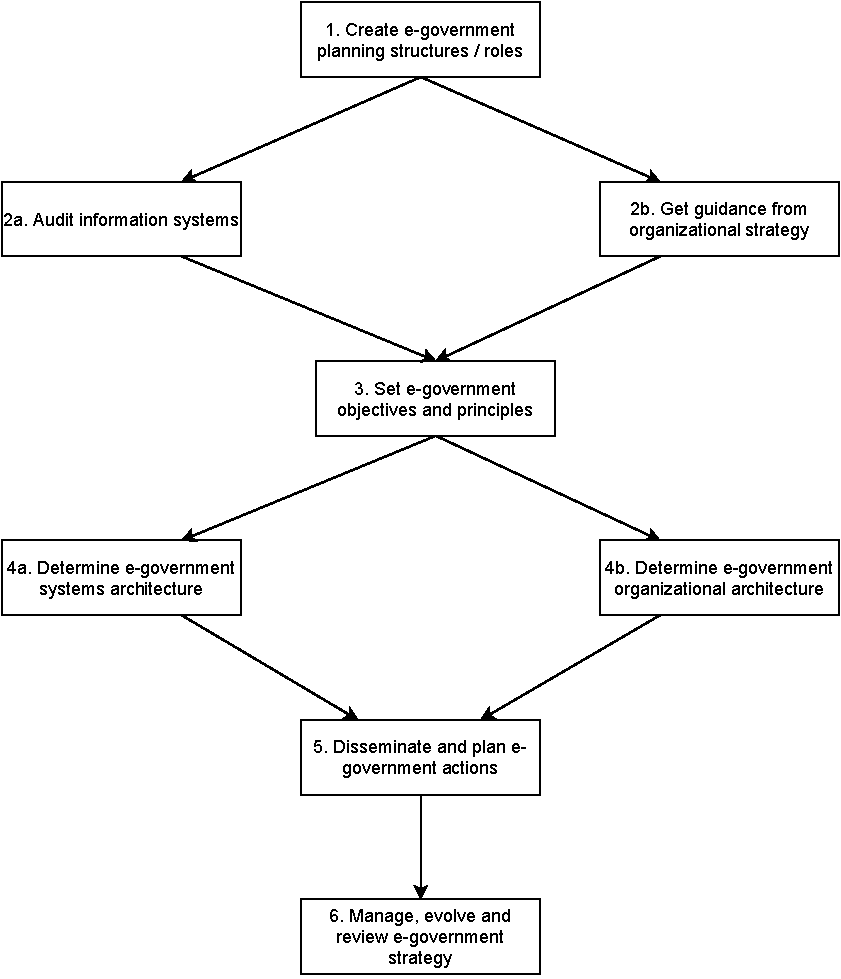
\includegraphics[width=0.9\textwidth]{steps-e-gov-planning}
	\caption{The steps of e-government strategic planning}
	\label{fig:steps-e-gov-planning}
\end{figure}

\subsubsection{Strategy Foundation: Create eGovernment Planning Structures/Roles}
\begin{itemize}
	\item In order to control the process of strategic planning, a special body is usually set up,	called something like `eGovernment Steering Group’. 
	\item It will typically consist of senior staff or other powerful stakeholders
	from various parts of the organization, together with some technical advisors.
	\item this committee is likely to be chaired by a Chief Information Officer
	(CIO).
\end{itemize}

This body normally reports to the very
top levels of the organization because of the
strategic nature of its work, which includes:

\begin{itemize}
	\item setting the scope of, and commissioning the e-government strategy; 
	\item taking necessary strategic decisions relating to e-government systems (such as those presented during strategic	planning); 
	\item communicating the e-government strategy to the rest of the organization; \item ensuring the necessary resources are in place to achieve strategic objectives, and allocating those resources; and 
	\item monitoring and controlling the overall development and operation of
	e-government within the organization, and
	checking this against stated objectives.
\end{itemize}

\subsubsection{Strategic Analysis: Audit Information Systems}
An e-government-specific answer to the
question ‘Where are we now?’ requires a
comprehensive understanding of the current
state of e-government and other information
systems.

It includes all types of information system, manual or computerized: hence the title ‘audit information systems’ rather than ‘audit e-government’.


Information systems (IS) audit is often
conceived in a very narrow sense, just as
an inventory of IT within the public
agency: all computer applications with
their hardware, software, networks, physical location, licensing and ownership; and
often just security-related. However such an approach is far too narrow to form an effective analytical base for strategy. It must be expanded in several ways, as below:

\paragraph*{Systems perspective}
Audit must recognize the full information system, describing not just the technology resources, but also: 
\begin{itemize}
	\item the information that information systems deliver, 
	\item the information processes undertaken, and 
	\item the human resources involved,
	\item covering information skills (e.\ g.\ data gathering and presentation), IT skills (e.\ g.\	hands-on computing), and system development skills (e.\ g.\ systems analysis and design).
\end{itemize}


\paragraph*{Issues perspective}
The audit should be more than just a list of
resources, but should help identify key
issues that will inform and affect subsequent decision-making on e-government.
These might include a sense of important
problems or complaints facing the current
information systems, or an assessment of
emerging trends.

\paragraph*{Contextual perspective}
This includes the outer two layers of the
‘onion-ring’ (see Section \ref{sec:e-gov-as-information-system}) within the
audit.

\begin{itemize}
	\item It will look at management systems and structures within the public agency.
	\item It will look at IT trends and standards within the local environment. 
	\item It will review financial and other constraints specific to e-government systems change. 
	\item Perhaps most important, it will incorporate an understanding of relevant policies, guidelines and initiatives that impact on	e-government. 
\end{itemize}


\subsubsection{Strategic Analysis: Get Guidance From Organizational Strategy}
An e-government strategy should therefore be firmly rooted in one particular element from the organizational context: the wider organizational or business strategy for the whole agency.

Business strategy first asks, 
\begin{itemize}
	\item `Where are we now?’ An answer	would include details of the organization’s	current structure and functions; key client	groups; existing problems that need to be addressed; and important current and forthcoming factors – particularly policies and political priorities – within the internal and
	external environment.
	
	\item It next asks, `Where do we want to get to?’ An answer would include details of the organization’s objectives, and some vision
	of the future organization that will enable it to overcome current and forthcoming problems, and to achieve its objectives.
	
	\item Finally, it asks, `How do we get there?’ This would be achieved through a statement of management strategy about major changes to
	organizational structure and functions in order to reach its future vision.
\end{itemize}

\subsubsection{Strategy Framework: Set eGovernment Objectives and Principles}
The eGovernment Steering Group may use the data gathered so far to produce a broad statement of the role and objectives of information and of e-government within
the organization. This statement may be specific (tying e-government to particular organizational objectives) and/or it may be generic (a general statement of information
and IT principles). 


These objectives and principles can also be used to develop the criteria against which e-government proposals may be evaluated and/or prioritized.


\subsubsection{Strategy Definition: Determine eGovernment Systems Architecture}
eGovernment strategy can be seen as needing to lay out the ITPOSMO dimensions for the future (see Section \ref{sec:e-gov-as-information-system}) The information,
technology and process dimensions are
together seen as an \textit{e-government systems architecture}: a plan of the e-government systems that the organization will require in
future. This architecture forms a major element of ‘Where do we want to get to?’ for
e-government.


The e-government systems architecture
can be described in terms of the individual
e-government applications with details of
data capture, input, processing, storage and
output plus links to decision and action
processes (CIPSODA: see Section \ref{sec:e-gov-as-information-system}) 

It will also consist of a number of different models, including:

\paragraph*{Data model}
\begin{itemize}
	\item A data model showing the structure of unified, organization-wide data to
	which the e-government systems will	have access; 
	\item often illustrated using an entity-relationship diagram.
\end{itemize}

\paragraph*{Process model}
\begin{itemize}
	\item A process model showing the key activities of the organization that the e-government systems will either support or undertake; 
	\item often illustrated using a process	diagram.
\end{itemize}


\paragraph*{Data/Process model}
\begin{itemize}
	\item A data/process model showing the organization-wide connection between
	business processes and data entities, and the organization-wide movement of data
	that e-government systems will enable;
	
	\item often illustrated using a data flow diagram.
\end{itemize}


The e-government systems architecture will
also consist of organization-wide models
for:

\begin{itemize}
	\item \textbf{IT}, showing how computers will be sized
	and connected within the organization,
	and an outline of the software to be used;
	\item \textbf{data management}, showing how data
	capture, input, processing, storage and
	output functions will be divided across
	the IT architecture.
\end{itemize}

A summary of all the elements within the
e-government systems architecture is shown
in Figure \ref{fig:architecture-elements-e-gov}.


\begin{figure}[ht!]
	\centering
	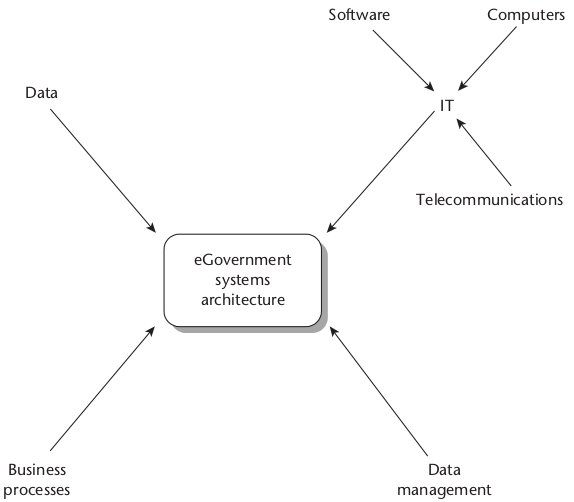
\includegraphics[width=0.8\textwidth]{architecture-elements-e-gov}
	\caption{Elements of e-government systems architecture}
	\label{fig:architecture-elements-e-gov}
\end{figure}


\subsubsection{Strategy Definition: Determine eGovernment Organizational Architecture}
General strategic decisions may include:

\begin{itemize}
	\item stating the approach to management of	organizational change, including a determination of the needs for cultural
	change;
	\item clearly allocating responsibilities for e-government systems development and
		management;
	\item identifying major competency gaps and	approaches to closing them through human resource strategies;
	\item deciding how back-office procedures may be restructured to support e-government;
	\item locating the e-government/IT function	within the wider organizational structure;
	\item demarcating which services (e.\ g.\ systems development, training and systems operation) are to be sourced in-house and outsourced;
	\item identifying procedures to be used when tendering for and selecting e-government systems products and services;
	\item specifying standard systems development methodologies and tools to be used; and
	\item identifying financial approaches to be adopted, such as public–private partnerships.
\end{itemize}


\subsubsection{Strategy Implementation 1: Disseminate and Plan eGovernment Actions}

The defined strategy can now be circulated as an ‘eGovernment Strategy Statement’ and,
if appropriate to the organizational culture, discussed and refined. 

Once agreed, the strategy is typically planned in more detail in a matrix format.

The columns of the matrix can be a set of e-government project plans, created for
improving existing systems and developing new systems. This might include:

\begin{itemize}
	\item a statement of project objectives; 
	\item an estimation of benefits, risks and constraints; and
	\item an estimation of resource requirements covering finance, human resources (i.\ e\. jobs and skills), technology, and timescales.
\end{itemize}

The rows of the matrix will be organization wide resource plans: 
\begin{itemize}
	\item for personnel training
	and development, 
	\item for finance, 
	\item for technology, etc.
\end{itemize}

\subsubsection{Strategy Implementation 2: Manage, Evolve and Review	eGovernment Strategy}
Strategic planning is not intended to be a
one-time activity but a continuous cycle
that needs to be completely revised at the
end of the strategic framework period, or
earlier if circumstances change or objectives
are not attained.

One task of the eGovernment Steering
Group is to monitor implementation of the strategic plan. Monitoring gathers
information on:

\begin{itemize}
	\item performance against objectives set for both e-government overall and individual
	e-government projects;
	\item benefits accruing to the organization	from e-government systems;
	\item problems related to developing or	operating e-government systems, with
	diagnoses and proposed remedies;
	\item other	impacts	associated with	e-government systems;
	\item changes to significant internal and external factors that affect the performance of the organization; and
	\item resources used and projected for use
\end{itemize}



On the basis of the information gathered, the eGovernment Steering Group may decide to modify the strategy.
%--------------------------------section end-------------------------




\section{Managing Public Data}
e-government systems are information systems. The data in e-government systems is therefore fundamental to the functioning of the public sector. It is too easy to assume that all is well with this data. Yet most e-government systems have data quality problems; sometimes so bad that they undermine the whole edifice of government functioning.

We can define data quality in terms of five `\textbf{CARTA}' indicators:

\begin{enumerate}
	\item \textit{\textbf{C}ompleteness}
	
	The degree to which all the data required by users is present in the e-government system.
	
	\item \textit{\textbf{A}ccuracy}
	
	The level of errors/incorrect data within the overall system data.
	
	\item \textit{\textbf{R}elevance}
	
	The degree to which data is necessary in order to complete particular	user decisions and actions.
	
	\item \textit{\textbf{T}imeliness} 
	
	The degree to which data can be delivered by the e-government system within a required time-frame.
	
	\item \textit{\textbf{A}ppropriateness of presentation} 
	
	The degree to which data produced by the	e-government system is accessible and intelligible to the recipient.
\end{enumerate}

\textit{The more CARTA the data, the higher its quality; the less CARTA the data, the lower its quality.}



It is estimated that around higher percentage of system data errors arise during the human elements of the process. Historically, this has occurred mainly during capture and input, because these were traditionally human-intensive tasks with errors arising from misreading, mistyping, and lost or omitted inputs. It has also
occurred after output, also because of misreading or misunderstanding.

But data errors can occur at any stage in the information cycle, for example, during processing, storage, output or transmission between those stages, as illustrated in Figure \ref{fig:poterntial-data-error-in-e-gov-cycle}.


\begin{figure}[th!]
	\centering
	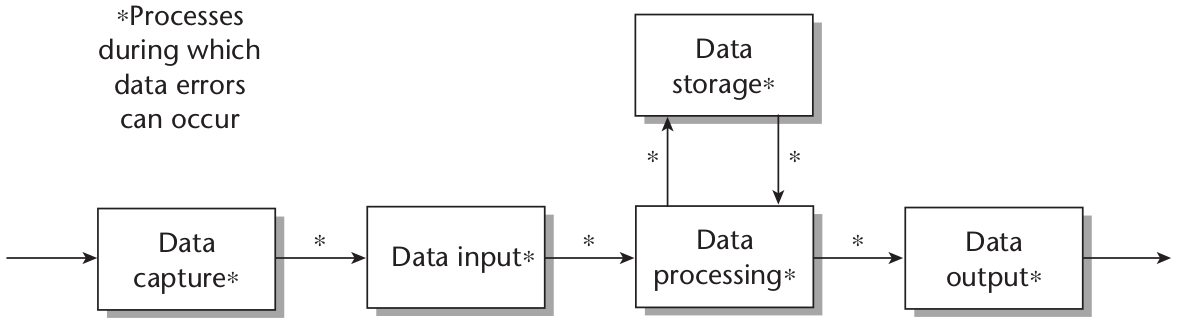
\includegraphics[width=0.8\textwidth]{potential-data-error-in-e-gov-cycle}
	\caption{Potential data error points in the e-government system cycle}
	\label{fig:poterntial-data-error-in-e-gov-cycle}
\end{figure}

In all cases, the data output will not be accurate or reliable. eGovernment systems with poor data will be prone to collapse as the poor data foundation undermines decision-making and action, as summarized in Figure \ref{fig:impact-of-inaccurate-data}.


This is often described as \textit{garbage in, garbage out (GIGO)}: what you get out from your e-government systems can only ever be as good as what you put in, and
if you put in garbage, you get out garbage. 

This is an issue for all organizations, but it is particularly an issue for the public sector and e-government:
\begin{itemize}
	\item The public sector is especially information intensive, and therefore relies heavily on data in order to undertake its	functions.
	\item The public sector often has responsibility for decisions that are critical to an individual's, a region’s or a nation’s welfare. 
	\item The public sector has legal obligations relating to data quality and accessibility, for example in relation to freedom of	information. 
	\item It therefore faces a significant threat of litigation if data quality is poor.
\end{itemize}

\begin{figure}[ht!]
	\centering
	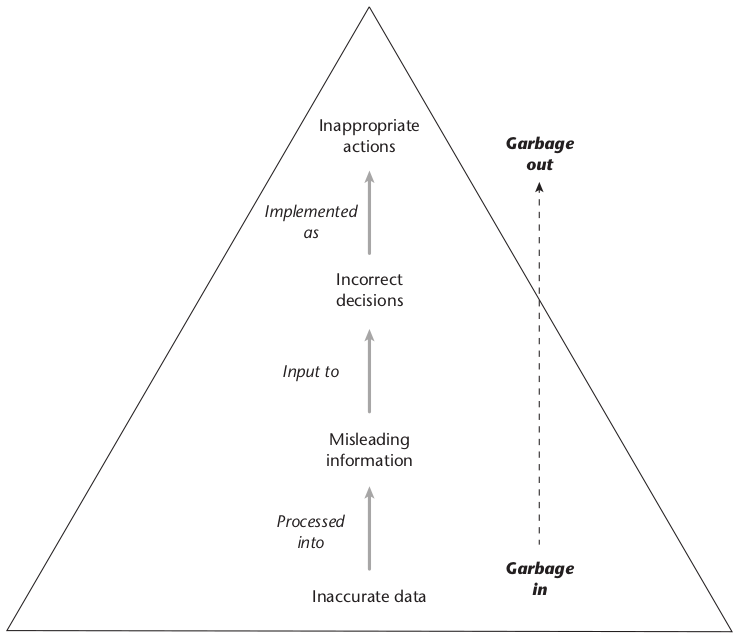
\includegraphics[width=0.7\textwidth]{graphics/impact-of-inaccurate-data}
	\caption{Impact of inaccurate data}
	\label{fig:impact-of-inaccurate-data}
\end{figure}

The public sector may also face additional constraints — on skills, on technology, related to the large size of its data sets — that increase the risks of data quality problem

\subsection{Causes of Public Data Problems}
We can divide causes into two main camps: 
\begin{enumerate}
	\item \textbf{hard}: technical causes of data quality problems and 
	\item \textbf{soft}: human causes. 
\end{enumerate}


\subsubsection[Technical Causes]{Hard Side: Technical Causes}
Looking first at the hard side, one can see that public managers love to blame data glitches on `computer errors', and that some technical problems do arise
which affect the data held by IT:


\paragraph*{Environmental hazards}
\begin{itemize}
	\item High temperatures and high humidity can cause hardware components to break down, thus corrupting data. 
	\item Static electricity can damage both electromagnetic components and corrupt data.
	\item Dust and smoke can short out components and make moving parts stick, especially damaging disk drives and the data on them. 
	\item Fire,	flood and lightning have a fairly obvious and catastrophic effect on IT-based systems.
\end{itemize}

\paragraph*{Electrical Problem}
\begin{itemize}
	\item Power spikes or surges (increases in voltage), and brownouts (decreases in voltage) can corrupt disk	held data and damage internal components. 
	\item Power cuts cause an ability to work, and a loss of all data in memory.
\end{itemize}


\paragraph*{Equipment breakdown} This can prevent data being exchanged or accessed.


\paragraph*{Software errors}
\begin{itemize}
	\item The presence of bugs (programming errors) in the software of an e-government system can have any number of effects. 
	\item These include overt or, worse, undetected corruption of data.
\end{itemize}


\noindent But to what extent can these truly be classified as `computer errors’ or technical problems? 

\subsubsection[Human Causes]{Soft: Human Causes}
The presence of bugs should be seen mainly as a problem of human, rather than technical, origin relating to the management of systems development. Even the actions of environmental or power hazards can often be traced to human inputs in the design, construction or operation of IT-based systems. This must put a question mark over the value of some hard approaches to public data quality.

We can reinforce this point by looking at another way in which technology could be blamed for inducing a further vulnerability and danger to data accuracy: the threat of computer crime.

Computer crime is a major problem for the public sector: 

\begin{itemize}
	\item internally, public employees are a significant source of such crime; 
	\item externally, threats seem to be growing and cyber-security has risen sharply up the agenda in many countries as a result of the terror attacks of the early $ 21^{st} $ century.
\end{itemize}


As well as entry of inaccurate data onto computer systems for personal gain, computer crime also includes:

\paragraph*{Alteration of existing data}
 For example, a worker increasing the rate of pay recorded for them in the payroll system, or the defacing.
 
 \paragraph*{Unauthorized access to existing data}
Hackers getting access to critical public data.

 \paragraph*{Deliberate destruction of data}
 For example, removing part of the organization's financial records just for the hell of it or introducing a computer virus.



\noindent Computer crime also covers physical theft of computer hardware or software (software piracy). Some public agencies even include personal use of organizational IT, such as typing and printing a personal letter or buying goods on the web from your office PC.


\subsubsection[Hard Solutions]{Hard Solutions to Public Data Quality Problems}
Hard, technical response to problems of data accuracy, including computer crime requires the imposition of various controls. These can be divided into two groups: 
\begin{enumerate}
	\item \textbf{general controls}, which affect all e-government systems; and 
	\item \textbf{application controls}, which relate to one particular e-government system.
	
\end{enumerate}


\paragraph*{General controls}

\begin{itemize}
	\item \textbf{Access controls}:
	\begin{itemize}
		\item Used to control user access to physical or digital components	of an e-government system. 
		\item Examples include security guards and passwords.
	\end{itemize}

\item \textbf{Communication controls}:
\begin{itemize}
	\item Used to control user access over computer networks.
	\item Examples include encryption and firewalls.
\end{itemize}
\item \textbf{Other technology controls}:
\begin{itemize}
	\item Such as controls to address virus, fire or power issues.
\end{itemize}
\end{itemize}


\paragraph*{Application controls}
To prevent many kinds of problems, many public agencies use application controls. The most important of these are \textbf{input controls}; that is, controls on the process of data entry that can be built into the e-government system. In many cases, if the control is violated, a customized message will appear providing guidance on the problem, and the new record will not be accepted until the error is corrected. 

Typically, the controls operate on each field within a database record and are stored as rules associated with that field.


\subsubsection[Soft Solutions]{Soft Solutions to Public Data Quality Problems}
We could identify a different role for each one of the CIPSODA (see Section \ref{sec:e-gov-as-information-system}) elements of an information system. However, that model can be simplified somewhat to produce the summary shown in Figure \ref{fig:data-roles}. This removes the roles of storage and output (because technology normally fulfils those roles) and merges the roles of decision maker and actor into the term `user'.


\begin{figure}[bh!]
	\centering
	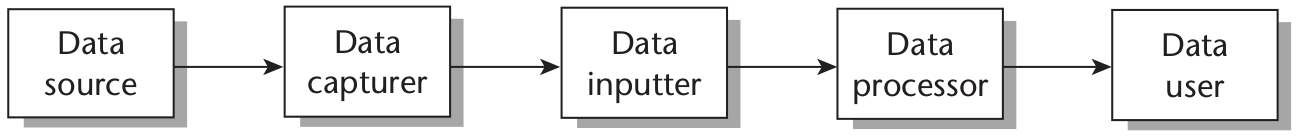
\includegraphics[width=0.8\textwidth]{data-roles}
	\caption{Different data roles played by people in public data systems}
	\label{fig:data-roles}
\end{figure}


The people occupying each one of these roles will have a different perspective on data, and we can develop a simple model of this, shown in Figure \ref{fig:soft-perspective-on-data-quality}. The model sees perceptions about how data is or is not used as shaping the motivations of each stakeholder which, in turn will shape their actions which, in turn will have an impact on data quality.


\begin{figure}[ht!]
	\centering
	
\includegraphics[width=0.8\textwidth]{graphics/soft-perspective-on-data-quality}
	\caption{A soft perspective on data quality}
	\label{fig:soft-perspective-on-data-quality}
\end{figure}

The soft perspective therefore argues that one of the keys to data quality, or lack of it, lies in the motivations of those involved. Where they are motivated to do so, those
involved will help data quality to be high. Where they are motivated to do otherwise, data quality is likely to suffer.


Some examples of perceptions — and their related motivations — will illustrate:

\paragraph*{Perception of data irrelevance}

\begin{itemize}
	\item Sources in public data systems, such as those asked to take part in a census or other survey, are often asked to provide data that is for the use of someone other than themselves. 
	\item Similarly, those capturing, entering and processing data are often treated as clerical automata, merely transmitting data to be used by some senior official. In such
	situations, the humans involved see the	data as largely irrelevant to their own work and their own lives, because they never use it. 
	\item As a result, they have limited motivation to worry about data quality, and their actions — for example, lack of care in response, or lack of concern about data entry errors — may undermine data quality.
\end{itemize}


\paragraph*{Perceptions of non-use}
This is related to the perception of data irrelevance. 

\begin{itemize}
	\item In some e-government systems, those involved know (or believe) that the data they are giving or collecting or inputting or processing is never actually going to be
	used. 
	\item This will have a knock-on effect on data quality.
	\item Within the politicized context of the public sector, for example, data entry staff may know that the data they type in is not	used; perhaps because senior officials make decisions using informal, political data rather than rational data from the computerized e-government system. 
	\item In that case, perfectly logically, the data entry staff will not be motivated to care about ensuring accuracy of the data they type in. 
	\item Alternatively, take the case of residents asked to provide input to the planning of a community policing strategy.
	\item Having once taken the trouble to provide data, they might feel that their efforts have produced no discernible result if no sensible strategy emerges. 
	\item Feeling their data was not going to be used they might, in the future, be motivated to refuse to provide further data to the police service.
\end{itemize}



\paragraph*{Perceptions of data-related punishment}

\begin{itemize}
	\item Citizens and businesses perceive that providing accurate financial data will lead to a punishment: their having to pay tax. 
	\item They are therefore motivated to withhold data (by	not providing a tax return, or not providing a full tax return); or to distort data (e.\ g.\ to	underestimate their income/profit or overestimate their expenditure/losses). 
	\item Any situation in which information is felt to have a political value may also lead to it being withheld on grounds of the old adage `information is power'.
\end{itemize}


\paragraph*{Perceptions of other data-related rewards}
\begin{itemize}
	\item Where performance-related pay has been instituted in the public sector, staff will rightly perceive that the provision of certain performance data (i.\ e.\ apparent performance above target) to their managers will lead to some personal reward (i.\ e.\ a pay bonus). 
	
	\item In this situation they will be motivated to hide negative performance data and to inflate or make up positive performance data, thoroughly undermining the performance management system. 
	
	\item Conversely, political leaders may be motivated to paint a falsely negative picture of difficulties in their district if they believe this will trigger a flow of assistance and development resources from federal or international funds.
\end{itemize}


\noindent These reward and punishment perceptions particularly affect the public sector and its clients (to whom it will often be providing money, services or other resource rewards), and compliers (whom it will often be `punishing' via a gamut from tax bills through fines or license revocation up to imprisonment). In all these cases, the citizen’s self-interest dictates that they will not be motivated to not present or handle data accurately.


All this assumes that those involved do have some perceptions, but there may be situations in which there is a lack of perception; for example, where sources do not know why data is being sought from them. They will try to work this out from situational clues, but they may guess wrong and accordingly skew the data they provide wrongly. Equally, there can be cases of lack of knowledge; for example, where sources feel motivated to provide data even though they do not have that data.


\subsubsection{Improving Public Data Quality}
what would the soft approach advocate as a way to address data quality problems in e-government systems? The key will be the perceptions and motivations of all those
involved in the chain. In particular, the public agency needs to find ways to align perceptions and personal motivations with formal organizational objectives.

What mechanisms exist for doing this? Some suggestions follow, summarized in Figure \ref{fig:soft-approach-data-quality}.
\paragraph*{Ensure there is a user}
\begin{itemize}
	\item Perception of data non-use is a major demotivator. 
	\item Matters can be improved if the e-government system is redesigned to ensure that the data being gathered is actually used for decisions and actions. 
	\item This may involve changing the content of data gathered to match the true information needs of users.
\end{itemize}

\paragraph*{Merge stakeholder roles}
\begin{itemize}
	\item The greater the number of stakeholders in the chain, the greater the chance of motivational problems. 
	\item Merging roles will reduce this danger. 
	\item Those who capture the data can also be those who input the data. 
	\item For example, where a survey was being	undertaken, role merger could mean the use of handheld devices that can accept data input in the field.
	\item Going further, data sources can themselves capture and input data.
	\item Where the consumers of public services themselves become producers of their own data, the use of web-based electronic	forms enables this.
\end{itemize}

\paragraph*{Make early stakeholders into data users}

\begin{itemize}
	\item Sources, capturers and inputters typically do not use the data that depends on them. 
	\item If they are turned into users, they have a much greater motivation to ensure the quality of system data.
\end{itemize}


\paragraph*{Other feedback to early stakeholders}
\begin{itemize}
	\item Even if early stakeholders do not become data	users, other types of feedback can motivate them. 
	\item This can be as little as a simple word of thanks from the user, or an explanation of why and how the data	is being used.
\end{itemize}

\paragraph*{Other reward and punishment techniques}
\begin{itemize}
	\item Giving money to data sources and higher pay to data capturers, inputters and	processors is one motivational technique, but money is not the only motivator.
	\item Punishment too can play a role, such as realistic threats of fines or imprisonment for those failing to fill or filling inaccurate tax returns, or threat of removal/reduction of budget by an audit or for failure to produce accurate audit figures.
\end{itemize}

\paragraph*{Find alternative sources}
\begin{itemize}
	\item Identify alternative sources for the same or similar data, who/which have less self-interest in the use of the data.
	\item For example, get administrative staff to return data on service activities of professionals (e.\ g.\ number of clients met) rather than the professionals themselves.
\end{itemize}


\begin{figure}[th!]
	\centering
	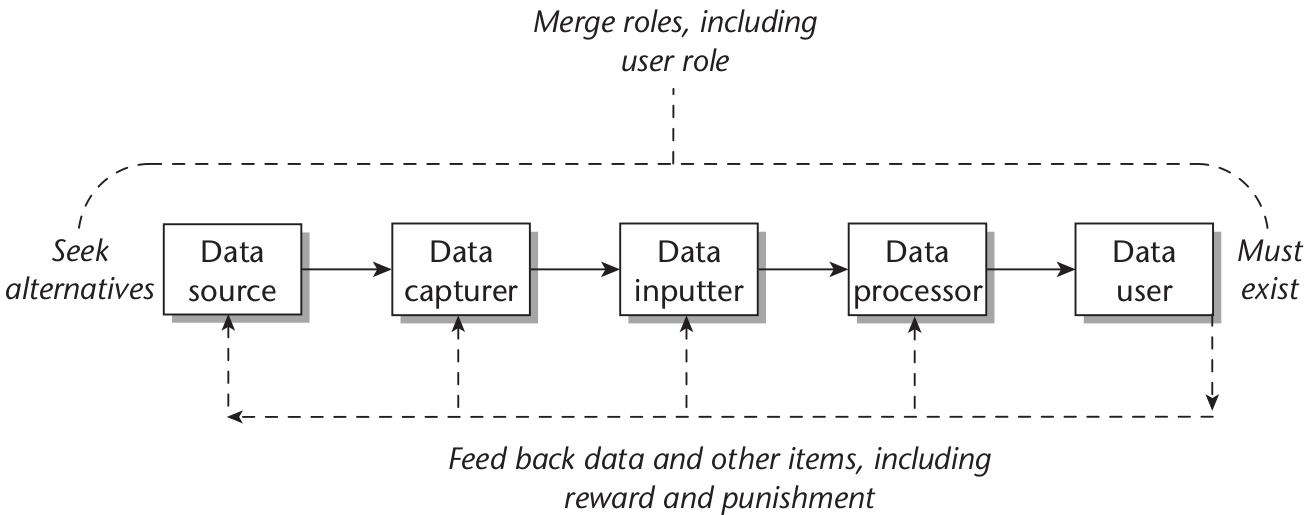
\includegraphics[width=0.9\textwidth]{graphics/soft-approach-data-quality}
	\caption{Soft approaches to improving data quality}
	\label{fig:soft-approach-data-quality}
\end{figure}



 %--------------------------------section end-------------------------
 
 \section{Managing Issues for e-Government}
 
\subsection{Core Issues}
Following are core issues that managers in the public sector have always faced:
\begin{itemize}
	\item position (the location of the IT function	within public sector organizations);
	\item people (recruitment and retention of staff involved with e-government);
	\item pelf (dealing with the financial aspects of e-government);
	\item projects (the ways in which e-government projects are managed);
	\item politics (the role of organizational power and politics in e-government).
\end{itemize}

\subsubsection{Position}
Where in the organization is the IT function to be located? There are various different possibilities.
\begin{itemize}
	\item Decentralized location,
	\item Centralized location,
	\item Hybrid approaches to IT location.
\end{itemize}

\paragraph*{Decentralized location}
At the extreme, responsibilities for e-government may be so decentralized that no organizational IT structures, staff or budgets exist: everything is left up to individual staff. 
\begin{itemize}
	\item One stage up from this is the situation in which one member of staff in each section is identified as the computer ‘whizz-kid’. 
	\item While continuing to perform their usual managerial or clerical role, they	informally take on an IT1 support role. 
	\item One stage further up, some or all of the organization’s departments have their own IT staff and/or IT unit and a specific departmental IT budget. 
	\item These resources are focused on serving the needs of the individual departments.
\end{itemize}


\paragraph*{Centralized Location}
At the other extreme is the centralized IT unit. 

\begin{itemize}
	\item Such units are normally funded from a	central budget. 
	\item They are naturally larger than their decentralized counterparts. 
	\item They may therefore be divided internally into a number of sub-units covering specialisms such as computer and network operations, systems development, data management, and strategic planning.
\end{itemize}

The location of the IT unit within the
overall structure of the organization reflects
attitudes to e-government in the organization, and also partly determines what the
unit can and cannot achieve within the
organization.


\paragraph*{Hybrid approaches to IT location}
Looking within the public agency, a hybrid location can mean either a separation or
integration of central and local responsibilities. For example, there could be a hybrid
management structure for the IT unit, with a management group that involves internal
users and senior officials as well as IT staff.

Alternatively, a hybrid structure for the IT unit could mean that it reflects the wider
structure of the public agency. Thus, for example, a unit supporting a local government could have a team covering housing, another team covering public works, another covering environment, and so on.


\subsubsection{People}
People are more important than technology. eGovernment managers must therefore spend much of their time dealing with people related issues.

The planning, development and operation of any new e-government system is likely to require new competencies, thus creating a gap between the competencies staff currently hold and those they need.

Competencies can be understood in relation to three domains:
\begin{enumerate}
	\item \textbf{Skills}: Organizations may find a skills gap in anything 
	\begin{itemize}
		\item from spotting opportunities for new e-government systems, 
		\item to analyzing current use of information, 
		\item to process redesign, 
		\item to software programming, 
		\item to system installation and use.
	\end{itemize}

	\item \textbf{Knowledge}: Organizations may therefore find a knowledge gap where staff do not know:
	
\begin{itemize}
	\item about systems development methods, or 
	\item about the nature and role of information and information systems, or 
	\item about organizational systems and processes, or 
	\item about	the basics of IT, or 
	\item about the design options that could be applied to the new e-government system, or 
	\item about why the new system should be operated in a particular way.
\end{itemize} 

\item \textbf{Attitudes}:
\begin{itemize}
	\item Where different stakeholders have different attitudes to the new e-government system, 
	\item one could talk of	an `attitude gap'. 
	\item In many ways this	reflects the different values and objectives of different stakeholders.
\end{itemize}
\end{enumerate}


Public managers face two main options in filling these competency gaps that new e-government systems create. They can:
\begin{enumerate}
	\item Train existing staff,
	\item Recruit new staff.
\end{enumerate} 


\subsubsection{Pelf}
Money matters loom large in e-government projects. For example, e-government has to work within the confines of public sector budgeting procedures. Related to this, e-government also has to work within the confines of available finance.

 \subsubsection{Projects}
The overriding management issue for e-government projects should be the challenge of failure. 
\begin{itemize}
	\item Most e-government initiatives fail due to poor implementation and management.
	\item Gaps between design and reality help to explain why e-government systems succeed or fail.
\end{itemize}


\subsubsection{Politics}
e-government is far more about people and politics than it is about technology and rationality:

Sometimes, IT projects fail because of economic reasons; rarely, if ever, because of technological factors. Most usually, the failures are political in nature.

Why should there be so much politicking around e-government? In short, because two pre-conditions of politicking\footnote{the action or practice of engaging in political activity.} are met.

\begin{enumerate}
	\item First, there are interdependent groups that have different objectives and values. 
	\item Second, there are important but scarce resources involved.
\end{enumerate}

So e-government brings together in large amounts both critical tangible resources — people, money and equipment — and critical intangible resources — information, power and kudos. They therefore form a key locus\footnote{a center of activity, attention, or concentration} for organizational politics.

%--------------------------------section end-------------------------


\section{Emerging Management Issues for e-Government}

Followinga are the management issues that have come to prominence more in recent years. 
\begin{enumerate}
	\item \textbf{performance} (the measurement of e-government-related performance);
	\item \textbf{policies} (the organizational policies that e-government managers have to develop	and promote); these are divided into:
	\begin{itemize}
		\item \textbf{policies on public data}, and 
		\item \textbf{policies on	other issues}.
	\end{itemize}
	 
\end{enumerate}

 \subsection{Performance}
 \begin{itemize}
 	\item Performance management is a component of public sector reform. 
 	\item It is a technique originating in the private sector that is now being promoted in the public sector. 
 	\item As with most such techniques, issues arise because some of the assumptions underlying performance management do not apply, or apply differently, in the public sector.
 \end{itemize}

\begin{figure}[ht!]
	\centering
	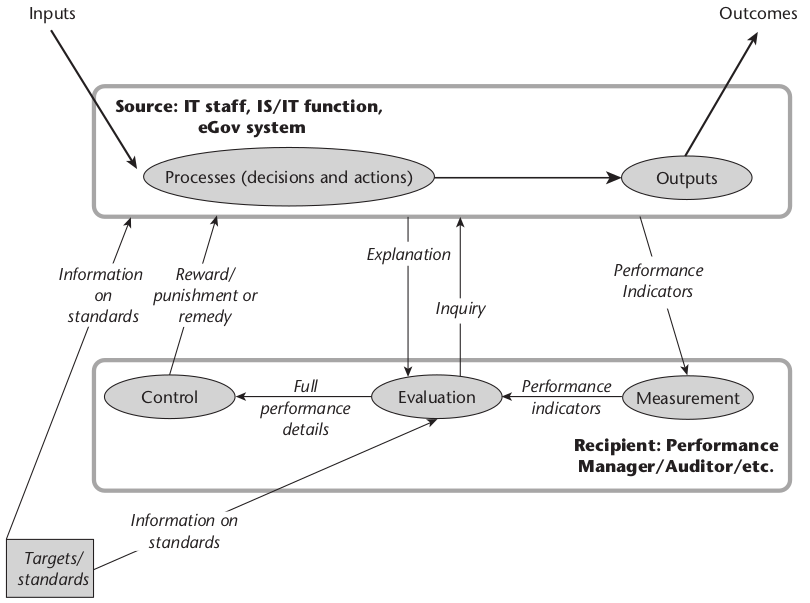
\includegraphics[width=0.8\textwidth]{perfromance-management}
	\caption{Performance management in e-government}
	\label{fig:perfromance-management}
\end{figure}

\subsubsection{Staff Performance}
Performance management in the public sector follows a standard pattern of target
setting, measurement, evaluation and control, as shown in Figure \ref{fig:perfromance-management}.


\begin{itemize}
	\item In reference to IT staff management, this would involve working first on a clear job specification and then tying the major items of content (ideally those that are output related) down to measurable performance indicators and targets. 
	\item Actual measures of performance would typically be discussed as part of regular staff-manager meetings with reasons for under and over-achievement discussed. 
	\item Rewards would be instituted for achievement/over achievement and remedial measures for
	under-achievement.
\end{itemize}

\subsection{Policies}
\subsubsection{Policies on Public Data}
 Public agencies operate in a sea of government laws, orders, policies and regulations. These external drivers pressurize agency e-government managers to develop and implement their own internal policies on
 a wide variety of issues.

Data policies must grapple with a four way data conflict faced by public agencies, summarized in Figure \ref{fig:data-conflicts}.

\begin{figure}[th]
	\centering
	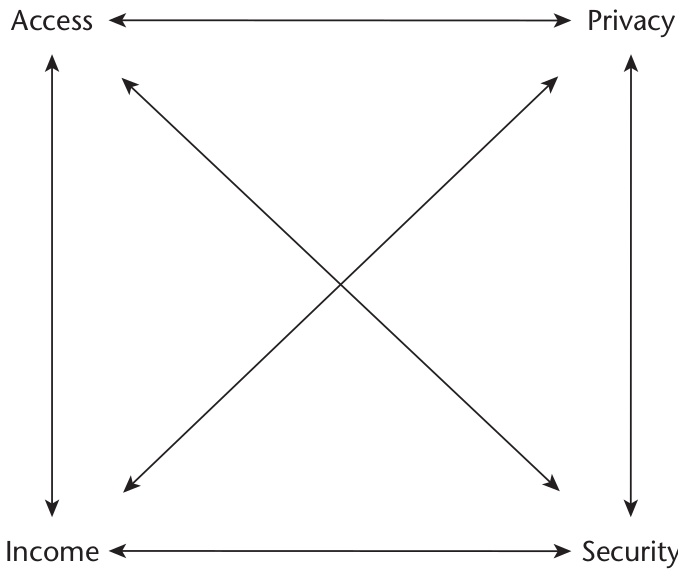
\includegraphics[width=0.6\textwidth]{data-conflicts}
	\caption{Data conflicts in the public sector}
	\label{fig:data-conflicts}
\end{figure}


Take the income–access tension: `Open government encourages making access easier and cheaper, while financial pressures on Departments and Agencies to recover costs and maximize returns on their information ``assets'' lead to controls and charging’. The more the government charges for its data, the greater the barriers to access become. Yet the wider it allows access, the less it can earn from data sales.


Following are some of the central policies that relate to access, privacy and security.

\paragraph*{Access policies for management of data records}
There are two main issues that public CIOs face in creating policies for data access: 
\begin{multicols}{2}
	\begin{enumerate}
		\item storage and 
		\item retrieval.
	\end{enumerate}
\end{multicols}



\begin{enumerate}
	\item \textbf{Storage}:
	As regards storage, public servants have to	be persuaded to treat digital data — from email messages to websites — in the same	way that they treat paper: `there has to be an audit trail, with version numbers for documents, which should be archived in read-only files so that they can't be tampered with'. Those electronic files must then be held securely and passed over to the archivists at the appropriate time.
	

\item \textbf{Retrieval}:
The second problem arises with retrieval. Data from old storage format such as CDs, and magnetic drive will be difficult access time goes. These devices lose their data after some years and these must be copied to new system. As the pace of technological change and the use of IT in government increases, this problem will only grow.

\end{enumerate}
\paragraph*{Access policies for freedom of information}
In a bid to ensure access to data across the public sector (and beyond) some governments have introduced \textit{freedom of information (FOI)} legislation.

\paragraph*{Access policies and the digital divide}
IT is very much a two-edged sword as regards access to government data. 

\begin{enumerate}
	\item On the one hand it reduces barriers. IT has made it far cheaper, quicker and easier to access that data (such as downloading electronic forms from government website instead of buying paper based form). 
	\item On the downside, IT raises barriers and has created a digital divide across which one group reaps the benefits of IT-enabled accessibility and one group cannot.
\end{enumerate}

\paragraph*{Privacy policies for data protection}
Data protection legislation chimes very much with information resource management principles, and it has been a significant driver behind centralized data management. It has pressurized public agencies to identify someone senior and central who will be responsible and accountable for the accessibility, confidentiality and accuracy of data held on e-government systems.

\paragraph*{Security policies for protection of data}
From Figure \ref{fig:data-conflicts}, we can see security may be in tension with goals of access and/or income.

The growing use of websites within e-government systems followed by the rise in global terrorism plus high-profile computer crime cases has thrown the issue right to the top of the management agenda.


\subsubsection{Policies on Other Issues}

There are many other policy issues of relevance to e-government. Here, we discuss three:
\begin{multicols}{3}
	\begin{enumerate}
		\item disability/accessibility; 
		\item ergonomics; and 
		\item Internet usage.
	\end{enumerate}
\end{multicols}

 
\paragraph*{Disability/Accessibility}
New technology offers ways to overcome some of the barriers faced by people with disabilities; including barriers of access to government data and government services. 

The policy requirements that relate to accessibility fall into two main types. First, there are very specific guidelines, such as those provided for e-government website design (e.\ g.\ `avoid using images to display text', `avoid using absolute sizes for fonts', `specify the language of text', `avoid using emoticons'. Second, there is a set of higher-level issues:

\begin{itemize}
	\item \textbf{Structures}: 
	\begin{itemize}
		\item A designated agency official responsible for accessibility policies, processes and structures; 
		\item an external voluntary advisory committee on disability and accessibility.
	\end{itemize}

\item \textbf{Systems}:  Processes and structures for feedback on accessibility including an email	contact and a system for complaints and for dispute resolution.
	
	\item \textbf{Processes}: 
	\begin{itemize}
		\item Training of staff to raise accessibility awareness and skills; 
		\item ensuring procurement of compliant technology; testing of web pages and other IT before
		live use in e-government systems; 
		\item reviewing kiosks for accessibility barriers.
	\end{itemize}

\end{itemize}

\paragraph*{Ergonomics}
Ergonomics can be defined as using knowledge of humans' physical and psychological technology, the arrangement of the work environment, and the organization of the job. By applying ergonomics in the design of e-government systems, health problems can be reduced and efficiency can be increased. 

\paragraph*{Internet usage}

As public servants spend increasing amounts of their working lives online, public agencies have been pushed to develop policies guiding online activity. As with many e-government-related policies, the driver for Internet use policy often seems to come from outside public agencies. It may be partly the drive of fear of litigation; it may be partly the drive of guidance from central agencies and it may be partly mimetic effects that spread from one agency to another. The overriding issue in all cases, though, seems to be concerns about the `cyber-liability’ of public agencies. 

Liabilities may cover civil issues (such as defamation by a public servant via an email or website, or email harassment) or criminal issues (such as obscenity, spreading of computer viruses, or breach of copyright, data protection or other relevant legislation).
 %--------------------------------section end------------------------- % ch-6: Managing e-Government
\chapter{Implementing e-Government}
\section{e-Government System Life Cycle and Project Assessment}
\subsection{System Life Cycle}
Innumerable methods for systems development have been created, with a variance
here or there, but all of them correspond
more or less to four core stages:

\begin{itemize}
\item \textbf{analysis} of what is currently happening, and
of whether and why a new e-government
system is needed;
\item \textbf{design} of the new e-government system’s
components;
\item \textbf{construction} of the new e-government
system;
\item \textbf{implementation} of the new e-government
system.
\end{itemize}

Any e-government systems project seeks to create a new situation that is different from the current one. The greater the difference between the new and current situations, the greater the degree of change that is required, and the greater the likelihood of system failure. Successfully planned e-government systems will therefore be those that require a manageable degree of change. 

In order to assess this `degree of change', the core of the systems development method consist of three activities:

\begin{enumerate}
\item mapping out the realities of the current
situation;
\item designing a proposal for the new situation; and
\item assessing the difference between the two,
and reacting to that difference.
\end{enumerate}


eGovernment projects typically involve a cycle of five stages: 
\begin{multicols}{2}
	\begin{enumerate}
		\item project assessment,
		\item analysis of current reality, 
		\item design of the new system, 
		\item system construction, 
		\item implementation and beyond.
	\end{enumerate}
\end{multicols}


%%%%%%%%%%%%%%%%%%%%%%%%%%%%%%%%%%%%%%%%%
%
%			FIGURE						
%
%%%%%%%%%%%%%%%%%%%%%%%%%%%%%%%%%%%%%%%%%
\begin{figure}[ht]
	\centering
	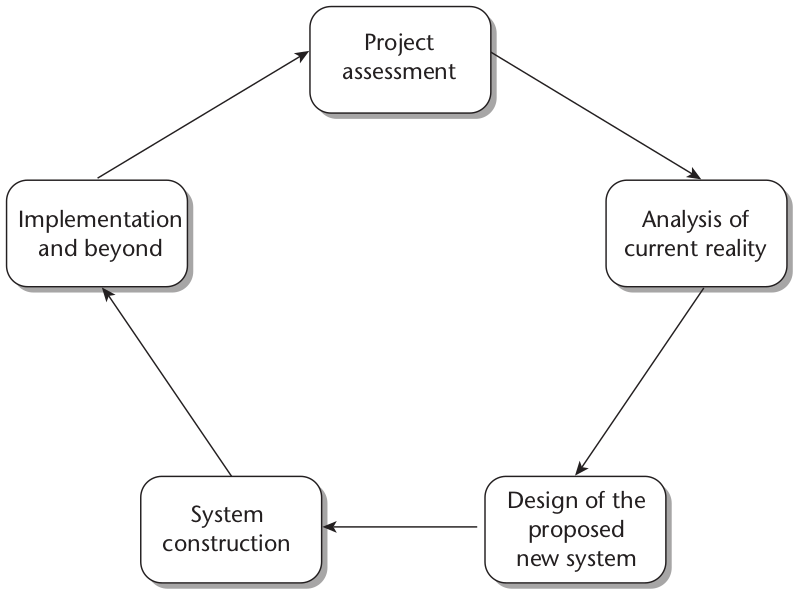
\includegraphics[width=0.9\textwidth]{e-gov-sdlc}
	\caption{The e-government systems development lifecycle} \label{fig:e-gov-sdlc}
\end{figure}

\begin{enumerate}
\item \textbf{Project assessment}: Identifying possible e-government projects; outlining basic project parameters; and assessing whether or not to proceed with the project.


\item \textbf{Analysis of current reality}: Description and analysis of the seven ITPOSMO
dimensions as they exist within the current situation of the organization.

\item \textbf{Design of the proposed new situation}:
Setting objectives for the proposed new
e-government system, and then describing in general terms how the seven
ITPOSMO dimensions should be different for the new system to meet these
objectives. Different options for the new
system may be evaluated at this point.

\item \textbf{System construction}: Acquiring any new
technology; undertaking detailed design
of the new system; then building it, testing it and documenting it.

\item \textbf{Implementation and beyond}: Training users
to use the new system; converting data
to new formats; introducing the new
system; monitoring and evaluating its
performance and context; then undertaking any necessary system maintenance.

\end{enumerate}


Assessing and mitigating risks (the degree of change between current reality and new
proposal design) is identified as a separate
activity. It could take place after general
design. However, in practice, risk-related
techniques are normally undertaken as an
integral part of stages 1 to 3.

Overall, the stages can be called a `systems development life cycle' because the post-implementation stages may lead to the identification of a new e-government project, thus restarting the whole process
again. The life cycle is shown in Figure \ref{fig:e-gov-sdlc}.

In practice, no method is as neat as this diagram might suggest because of two things.
\begin{itemize}
	\item First, \textbf{parallelism}: activities running simultaneously. For example, analysis of current reality and general proposal design tend to	overlap, with continuous analysis of the
	gap between the two. 
	\item Second, \textbf{iteration}: looping back from a later step to an earlier one. For example, an issue thrown up	during analysis of current reality may alter the basic project parameters and require	re-assessment of the project. Alternatively, a problem during system implementation	may lead to a realization that current reality needs to be re-analyzed and the e-government proposal redesigned.
\end{itemize}
%In practice, no method is as neat as this
%diagram might suggest because of two things. First, \textbf{parallelism}: activities running simultaneously. For example, analysis of current
%reality and general proposal design tend to
%overlap, with continuous analysis of the
%gap between the two. Second, \textbf{iteration}:
%looping back from a later step to an earlier one. For example, an issue thrown up
%during analysis of current reality may alter
%the basic project parameters and require
%re-assessment of the project. Alternatively,
%a problem during system implementation
%may lead to a realization that current
%reality needs to be re-analyzed and the
%e-government proposal redesigned.


No method is perfect but there are dangers for the public sector in adopting
some of the harder methods. The public sector has had a tendency to choose such
methods which then prove too old, inflexible, top-down, detailed, jargonized and time-consuming.

Some public sector organizations mandate that one method alone be used for
systems development. In other situations,
choice of method will depend on factors
such as:

\begin{itemize}
	\item \textbf{The system developer(s)}: Methods that a developer has experience of will be preferred to those that are new. Developers	also have innate preferences that are relevant. Some, for instance, will prefer hard methods; others will prefer soft methods.
	
	\item \textbf{The size of system}: Small e-government
	systems cannot justify such a comprehensive. Instead, one or two of the most relevant
	aspects only need be used. The larger the
	system, the more one can justify a
	greater systems development effort.
	
	\item \textbf{The nature of the organization}: More participative, human- or user-centered methods are difficult to apply in some
	public sector organizational cultures. In
	these cases, more top-down, centralized
	methods are likely to be employed.
\end{itemize}


\subsection{Project Assessment}
\subsubsection{Identifying a Project}
New e-government projects typically arise in one of two ways:
\begin{itemize}
    \item First, \textit{identification of a  problem} that needs to be solved.
    \item Second, \textit{identification of an opportunity} which could be seized.
\end{itemize}

Such problems and opportunities arise from many possible sources. These sources can be any of the factors. They can arise from the external environment or from internal sources. They can be
rational or political or personal. They can form part of a broader strategy or program/portfolio or stand alone.

\paragraph*{External examples include}
\begin{itemize}
	\item complaints from citizens, politicians or
	the media;
\item new legislation or directives or other
	pressures from external institutions,
	including those framed within the context of public sector reform;
\item external economic, political or social crisis;
\item technological innovation;
\item observation of sister organizations; or
\item the political need to project a more
	modern image for the organization.
\end{itemize}

\paragraph*{Internal examples include}

\begin{itemize}
	\item a previously conducted strategic planning exercise or consultancy report;
	\item a survey of staff problems or suggestions;
	\item shortfalls in work performance measures;
	\item financial resources being available that
	need to be spent on something before
	financial year end;
	\item an individual’s desire to give their career
	a boost; or
	\item an individual’s desire to earn kickbacks
	from IT suppliers
\end{itemize}

\subsubsection{Gathering Information on	the Project}
It describes the way in which information is gathered on a proposed
e-government project in order to assess
whether or not to proceed with it, using
a basic – who, what, why — approach. If required, these can all be compiled together
into an initial project proposal.

\paragraph*{Stakeholder analysis: who is involved?}
Stakeholders are those individuals or groups
who have a stake in the success of the new
project. It is they who are the main determinant of whether the project proceeds or is
scrapped, and of whether a project succeeds
or fails.

A a number of possible key stakeholders are summarized in Figure \ref{fig:stakeholder}.

\begin{figure}[th]
	\centering
	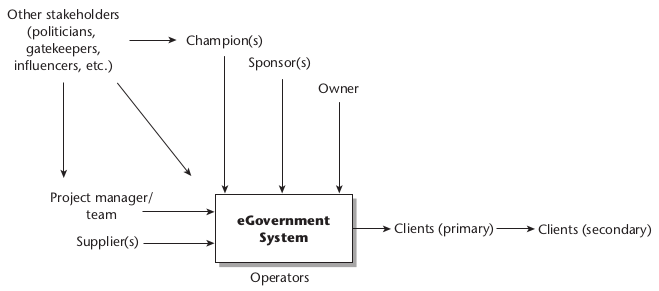
\includegraphics[width=0.8\textwidth]{stakeholder}
	\caption{Stakeholder map for an e-government project}
	\label{fig:stakeholder}
\end{figure}


The stakeholders are:

\begin{itemize}
	\item \textbf{Project manager/team}: Those who will analyze, design and build the e-government
	system.
	\item \textbf{Supplier(s)}: Those who will supply the technology and other resources required
	by the e-government system.
	
	\item \textbf{Operators}: Those who will be carrying out	the activities/processes that make the
	e-government system work.
	
	\item \textbf{Clients}: Primary clients are on the immediate receiving end of what the
	e-government system does or outputs. Sometimes these will be outside government (e.\ g.\  citizens or businesses). Sometimes, though, these will be inside	government (i.e. public servants)
	
	\item \textbf{Champion(s)}: The person (or group) who drives the project on and seeks to justify
	its implementation.
	
	\item \textbf{Sponsor(s)}: The person (or group) who pays for the expense and effort required
	to develop the new e-government	system.
	
	 \item \textbf{Owner}: The manager of the organization or department that will own and use the
	system, who is ultimately responsible for the system.
	
	 \item \textbf{Other stakeholders}: Who have a significant influence on the project or on
	whom the project will have a significant
	influence.
\end{itemize}

\paragraph*{Problem statement: what is the problem?}
It may be useful to create a problem statement: a single sentence that tries to encapsulate who or what
the problem relates to, and what exactly is
wrong, without trying to define a solution.
This statement may well be defined by the
most powerful stakeholders.

\paragraph*{Project Rationale: why?}
This is a simple definition, possibly in a
single sentence, of the main objective for
the new e-government system sought by the
most powerful stakeholders. In most situations it would relate to alleviating the previously identified problem (or making use of
the identified opportunity).


\paragraph*{Constraint analysis: what constraints?}
Constraint analysis helps you
understand the roadblocks that hold an
e-government project back.

Constraints will vary from situation to
situation. Example:

\begin{multicols}{2}
	\begin{itemize}
		\item Technology
		\item Objectives and values
		\item Staffing and skills
		\item Other resources
	\end{itemize}
\end{multicols}


\paragraph*{Environmental prediction: what next?}
A classic systems failure is to create a new e-government system suitable for today, but
not for tomorrow. To guard against this,
some type of ‘crystal ball gazing’ is required
to anticipate future conditions within which the e-government application will have
to operate. Typical points to be answered
include:

\begin{itemize}
	\item How long is the new system likely to last?
	\item How is the operation of the e-government system likely to change over its lifetime?
	\item What kind of changes are likely to occur within the system’s environment during this timeframe?
	\item Given all the changes, is the e-government system likely to be sustainable?
\end{itemize}

\subsubsection{Project Summary Statement}
In thinking about and discussing a potential e-government project, it can be useful
to have a single statement that summarizes
the project. Such statements need to be
concise enough to make them usable, but
comprehensive enough to include the
important aspects of the project.

\subsubsection{Assessing the project: the ‘business case’}

\paragraph*{Project Feasibility}
This is the first quick and dirty attempt to
check the gap that exists between current
reality and the new design required in order
to implement the proposed e-government
system. The intention is to look at risks in
order to assess whether or not it makes
sense to proceed with the project.

Focusing just on some key
points in the public sector, feasibility can be
corralled under the PoTHOleS acronym:
\textbf{P}olitics, \textbf{T}echnology, \textbf{H}ard cash (i.e. finance),
\textbf{O}ther \textbf{l}esser \textbf{r}esources, and \textbf{S}ustainability. Each
of these can be regarded as a pre-condition
for successful development and operation of
an e-government system:
\begin{multicols}{2}
	\begin{itemize}
		\item Political feasibility
		\item Technical feasibility
		\item Hard cash – financial feasibility
		\item Other lesser resource feasibility
		\item Sustainability
	\end{itemize}
\end{multicols}


\paragraph*{Project priorities}
One way to choose between projects is to
look at their assessed feasibility, and prioritize
those projects that look most feasible.

Ultimately, though, priorities may well be
determined by the personal objectives of
the most powerful stakeholders.



\paragraph*{Project opportunity costs}
Only rarely is the question asked: ‘What
else could we invest these resources in if we
did not invest them in this e-government
project?’ If the question is asked it can produce surprising results. Stakeholders may
suddenly become aware that a large amount
of money and time is about to be spent on
something that no-one particularly wants.


\paragraph*{Project impacts}
eGovernment systems are increasingly
interwoven into the fabric of the public
sector and, as a result, they have a growing
impact on the work of the public sector. At
this point in the lifecycle, then, impact
assessment exercises may be conducted,
such as the privacy impact assessments.


\paragraph*{Project planning and management: how, who, what and when?}
Once a decision has been made to proceed
further with an e-government project, plans
are normally made for that project. This will
typically involve decisions about:

\begin{itemize}
	\item \textbf{How}: The approach to systems development to be used; the main stages and
	tasks that will have to be undertaken in
	order to develop any new system; and
	the deliverables that form their output
	(reports, diagrams, decisions, acquired or
	developed IT, etc.).
	
	\item \textbf{Who}: The staff involved in systems
	development from both inside and outside the organization.
	\item \textbf{What}: The financial, technological and
	other resources that will be required for
	development.
	\item \textbf{When}: The timetable that will be worked
	to. Project milestones can be inserted as
	points for project review based on time
	(e.g. every week), money (e.g. after a
	certain amount has been spent), or on the
	deliverables (e.g. after the project assessment, after the analysis of current reality,
	etc.).
\end{itemize}

\section{Analysis of Current Reality}
\subsection{Methods of Analysis}
\subsubsection*{Overview of Data-gathering Methods}


There are four main data-gathering
techniques that can be used to understand
current reality: 

\begin{enumerate}
\item \textbf{Interview/discussion}: Talking to individuals
or groups about the current situation.

\item \textbf{Questionnair}e: Gathering background information using a survey of stakeholders.

\item \textbf{Document analysis}: Reviewing current
manuals, regulations, policies, contracts,
memos, reports, and so on.

\item \textbf{Observation}: Looking at what currently
goes on, including the use of any current
information systems.
\end{enumerate}

\subsection{Recording Techniques}
The elements described above can be recorded
as text. However, using diagrams offers some
significant benefits, because diagrams help to
simplify, formalize and communicate representations of public sector reality.


Diagrams may be used
primarily for eliciting rather than recording
information. First, because diagrams help
clients, staff and other stakeholders to
understand a situation more easily than
other means. Second, because diagrams are
interesting and therefore stimulate people to
contribute further. Key diagram techniques
are discussed below.


\subsubsection*{Reality-Specific Diagrams:	Rich Pictures}

A rich picture is a diagram rich in detail that
represents and summarizes the most important components of a government system
and its context. It is one of the few diagramming
techniques that helps represent current
reality, as opposed to some theoretical and
rational ideal.

\subsubsection*{Design/Reality Diagrams}
Can be used either to represent
current reality or to summarize the new
e-government system design.

It includes:

\begin{itemize}
	\item Process map
	\item Data flow diagram (DFD)
	\item Entity-relationship diagram (ER)
\end{itemize}



\section{Design of new e-Government system}
Too many e-government systems are
designed from a hard perspective — focusing
design on the technology, the data it
handles, and related public sector processes
only. Hard approaches are attractive because they are
relatively simple and easy, because they
reflect the ‘e’ in e-government, and because
they reflect the technical background of
many designers. However, hard approaches
often end in failure because they ignore the
soft human, political factors that have such
a critical impact on e-government projects.


A successful approach to e-government
design must therefore be a hybrid approach:
one that encompasses both hard and soft
elements; 

Following are five design headings:

\begin{multicols}{2}
	\begin{enumerate}
		\item objectives;
		\item information;
		\item technology;
		\item processes; and
		\item human systems (staffing, skills and management).
	\end{enumerate}
	
\end{multicols}


\subsection{Setting Objectives}
The design and development of a new e-government system requires some guiding framework. A project summary statement may provide this to some extent, but most
projects will require a set of objectives to work to. Taking account of the framework of constraints and future changes, these can be based on the previous problem statement, project rationale statement, problem analysis and/or personal objective setting.

Objectives are often stated in terms of the benefits sought from the proposed new e-government system, and may be a mirror image of any identified problems. Objectives for an e-procurement system, for example, could include:


\begin{itemize}
\item to reduce the time taken to procure goods and services;
\item to increase the accuracy of ordering and payment; and/or
\item to increase the motivation of purchasing section staff.
\end{itemize}

If there are a number of objectives, these can now be prioritized in order to provide a principal focus for subsequent system development.


\subsubsection{Information Design}
It should not be assumed that the information provided by any existing information
system meets current needs. Data may be
disseminated to clients because ‘we have
always done it that way’, even if that data is
of no value to either the client or the public
agency. Similarly, there may be information
that stakeholders would like to access, but
which is not being gathered or created.
Some analysis of information requirements
is therefore often appropriate.
The information required within the new
e-government system can be planned using
a set of questions about the key information
functions. 


\paragraph*{Output requirements}
How will information outputs meet system
objectives:

\begin{itemize}
	\item Who will expect output from the new
	system?
	
	\item What information will they require
	to be output from the system?
	
	\item Why do stakeholders require this information?
	\item How often and when and where will
	the e-government system be expected to
	produce information output?
	\item In what format will the system be
	expected to produce information output?
	\item What characteristics should the information output possess?
\end{itemize}

\paragraph*{Capture and input requirements}
How will input data meet output needs:
\begin{itemize}
	\item What data will have to be input to produce
	the required outputs?
	\item Where will the data come from, and in
	what form, in order to produce the
	required outputs?
	\item How will data be captured and input to
	the e-government system?
\end{itemize}

\paragraph*{Process requirements}
How will processing turn input data into
output information?

\paragraph*{Storage/Retrieval requirements}
How will storage hold data needed for
processing and output:
\begin{itemize}
	\item What data will be stored and retrieved in
	order to produce the required output?
	\item In what way does the data need to be
	stored?
\end{itemize}
\paragraph*{Communication requirements}
How will data be transmitted to support other tasks:
\begin{itemize}

	\item What data will be transmitted as part of
	the tasks of capture, input, processing,
	storage/retrieval and output?
	\item Where, or to whom, will the data be
	transmitted?
	\item How will it need to be transmitted?
\end{itemize}


\subsubsection{Technology Design}
This involves thinking through alternative
ways in which technology can meet stated
objectives and information requirements,
and selecting one of the alternatives. 

\paragraph*{Software design}
In designing the IT component of an
e-government system, software is typically
the first focus because it is software that actually does the work. If hardware is designed
first, there is a danger that it will not be able
to run the necessary software. Three design
choices must be made, as below.

\begin{enumerate}
	\item \textbf{Type of Application}
		\begin{enumerate}
			\item Improved data handling
			\item Improved decision-making
			\item Improved interaction
		\end{enumerate}
	\item \textbf{Method of Software Development}
	\begin{enumerate}
		\item Off-the-shelf package: This either works
		immediately on purchase or merely requires
		organization-specific data to be entered.
		
		\item Customized package: This is an off-the-shelf
		package that is altered to fit organization/user needs.
		
		\item Custom-built application: This is software
		built from scratch to meet organization/user needs.
		
		\item System re-engineering: This is the redesign
		and rewriting of an existing software application.
	\end{enumerate}
\item \textbf{Operating System}
\end{enumerate}

\paragraph*{Hardware design}
Three main design choices need to be made,
as below.
\begin{itemize}
	\item \textbf{Computer Size}
	\item \textbf{Specialist Hardware}
	\item \textbf{Information Systems Architecture}
\end{itemize}


\subsubsection{Process Design}
This involves thinking through alternative
ways in which organizational processes can
meet stated objectives, and selecting one set
of alternatives.

There are two groups of tasks that form
key e-government processes, and about
which decisions have to be made in an
e-government project:

\begin{enumerate}
	\item Core information system tasks: At least
	some of the tasks required will differ from
	those of `current reality’ because there is
	a move from an old to a new information
	system in e-government development.
	\item Wider system tasks: These tasks will be
	placed somewhere on the untouched —	optimized — redesigned — re-engineered
	continuum.
\end{enumerate}

\subsubsection{Human System Design}
This involves thinking through alternative ways of organizing work and work structures in the new e-government system in order to meet stated objectives, and selecting one set of alternatives. Whereas the process design phase focused on what is to be done, this phase focuses on how it is to be done, and by whom.


\subsubsection{Evaluating Proposals and Alternative Designs}
Evaluation
can mean identifying the extent of change
required between current reality and the
proposed design(s).

\section{e-Government Risk Assessment and Mitigation}
Most e-government projects fail in some way. It therefore makes sense
to perform some kind of risk assessment — and mitigation where necessary — within the
e-government system lifecycle.

In general terms, we can pose the following questions about risk assessment and
mitigation:
\begin{itemize}
	\item Why? The aim of risk management is to
	stop e-government projects failing.
	\item When? Assuming a typical project life-cycle of assessment–analysis–design–construction–implementation, then
	typically you would do a quick and dirty
	risk assessment during the assessment
	stage, and a more detailed assessment
	during the analysis stage.
	\item Who? A small team consisting of a mix of
	different stakeholders is the best unit to
	assess risk. The fewer people involved, the
	greater the chance that you miss an
	important risk. The more people involved,
	the higher the time and financial and
	other costs of the exercise.
	\item How? Focusing	on the notion of design–reality gaps.
\end{itemize}

\subsection[Risk Assessment]{Risk Assessment Through Gap Analysis}
It is not easy to analyze the gap between current reality and the design assumptions and requirements of a proposed new e-government
system. There are no hard and fast rules that
say `this gap is OK' or ‘this gap is too large’.
Any assessment of gaps — and, hence, of
project risk — must therefore be subjective,
and based on opinion and experience. If one
accepts this subjectivity, then rating scales
can be used, as described below:


\begin{enumerate}
	\item Using each of the seven ITPOSMO
	dimensions in turn, analyze two things.
	First, the organizational reality relating
	to that dimension that exists right now
	at the time of analysis. Second, the
	conceptions/requirements within the
	design of the e-government application.
	
	\item For each one of the dimensions, give a
	numerical rating to indicate the size of
	the design–reality gap on that dimension. The rating for each dimension’s
	gap can be anywhere on a scale from
	zero to ten.
	\begin{itemize}
		\item 0 rating would indicate \textit{no change}
		between the design proposal and
		current reality;
		\item 5 rating would indicate\textit{ some degree of
		change} between the design proposal
		and current reality;
		\item 10 rating would indicate \textit{complete and
		radical} change between the design
		proposal and current reality.
	\end{itemize}

\item The other six dimensions to be rated
from 0 to 10 are:
\begin{enumerate}
	\item the technology used by agency and
	clients;
	\item the work processes undertaken in the
	agency–client system;
	\item the objectives and values that key
	stakeholders need for successful implementation of the e-government application versus their current real objectives and values;
	\item the staffing numbers and skill
	levels/types required by the agency
	and clients;
	\item the management systems and structures required in the agency;
	\item the time and money required to successfully implement and operate the
	new application compared with the
	time and money really available now
\end{enumerate}
\item The simplest and crudest thing to do
now is to add up the rating numbers for
all seven ITPOSMO dimensions and
interpret them according to Table \ref{tab:risk-ratings}.
\end{enumerate}

% Please add the following required packages to your document preamble:
% \usepackage{booktabs}
% \usepackage{longtable}
% Note: It may be necessary to compile the document several times to get a multi-page table to line up properly
\begin{longtable}[c]{@{}lp{9cm}@{}}
	\caption{Risk ratings and outcomes for eGovernment projects}
	\label{tab:risk-ratings}\\
	\toprule
	\textbf{Overall rating} & \textbf{Likely outcome}                                                                                  \\* \midrule
	\endfirsthead
	%
	\multicolumn{2}{c}%
	{{\bfseries Table \thetable\ continued from previous page}} \\
	\toprule
	\textbf{Overall rating} & \textbf{Likely outcome}                                                                                  \\* \midrule
	\endhead
	%
	\bottomrule
	\endfoot
	%
	\endlastfoot
	%
	57–70                   & The e-government project will almost certainly fail unless action is taken to close design–reality gaps. \\
	43–56                   & The e-government project may well fail unless action is taken to close design–reality gaps               \\
	29–42 & The e-government might fail totally, or might well be a partial failure unless action is taken to close design–reality gaps \\
	15–28                   & The e-government project might be a partial failure unless action is taken to close design–reality gaps  \\
	0–14                    & The e-government project may well succeed                                                                \\* \bottomrule
\end{longtable}

\subsection[Risk Mitigation]{Risk Mitigation Through Gap Prevention or Reduction}

Risk assessment through analysis of gaps is
only one element. We also need to take
action if there are large gaps and a high risk
of failure. Options for action are summarized through \textbf{ZABC}:

\begin{itemize}
	\item \textbf{Z}ap the project: Abandon the e-government initiative.
	
	\item \textbf{A}lter the project: Change some of the initiative parameters to try to make it
	more feasible. 
	
	\item \textbf{B}e selfish: If the change initiative seems
	likely to fail but it cannot be zapped or altered, then focus on personal goals and
	personal gains that can be extracted from the initiative such as training, expertise
	and experience, money, or equipment.
	
	\item \textbf{C}hange your job: More radically if the e-government initiative seems likely to
	fail, change job either within the public agency to get away from the project, or
	to another organization
\end{itemize}


\section{e-Government System Construction}
Once a design for the proposed new
e-government system has been agreed, the
development cycle can proceed to the
remaining stages: that of actually constructing the new system and then implementing
it. The steps in system construction are:

\begin{itemize}
	\item acquiring any necessary new technology;
	\item undertaking detailed system design;
	\item constructing the new e-government	system, and
	\item testing and documenting the system.
\end{itemize}

\subsection{Procurement For e-Government System}
New technology now needs to be
acquired if any existing IT system is not suitable and
also, for software, if a new software package
(rather than re-engineered system) is to form
the basis of the e-government system.

The approach to acquisition needs to be
decided at the start. Five options are common in the public sector.

\begin{enumerate}
	\item \textbf{Expression of interest}: Based on an informal statement of the agency requirements. 
	\item  \textbf{Request for proposal}: Based on a more detailed statement of requirements than the Expression of Interest.
	\item \textbf{Request for tender}: With the detailed requirements and conditions to elicit a
	comprehensive and comparable response from suppliers.
	\item \textbf{Price quotation}: A simple price request from suppliers for a specific item or items.
	\item \textbf{Period contract arrangement}: This sets a
	time period for a relationship between
	public agency and supplier typically
	relating to the provision of particular
	goods and services, such as a software
	package or delivery of IT training.
\end{enumerate}

\subsection{Final Construction of The e-Government System}
The final construction of the system
involves the steps below.

\begin{itemize}
	\item \textbf{System Installation}
	
	Once the technology has been acquired, it
	will need to be installed. For larger e-government systems, this will require considerable pre-planning and site preparation.
	
	\item \textbf{Detailed System Design}
	
	If the software chosen as the basis for the
	e-government application is an off-the-shelf
	package, the system development process
	can proceed fairly directly to implementation (though testing and documentation
	will be required to some extent). If not,
	more detailed design work is required as
	a precursor to system construction or
	customization.
	
	It is at this point that specific design decisions can be made relating to issues, including
	design of:
	\begin{itemize}
		\item data-gathering exercises that will produce
		the required data for the organization;
		\item general controls to protect data quality;
		\item specific application controls, including
		validation parameters for each data
		element;
		\item codes to be used for particular data
		elements;
		\item other detailed operational procedures
		that may be required;
		\item input forms and screens;
		\item processing techniques required to produce information from data, with an
		emphasis on simplicity and flexibility;
		\item output screens and other output formats;
		\item other system interfaces, such as query
		screens; and
		\item system ergonomics
		
		Based on all these designs, the information
		system for e-government can now be
		constructed.
		
	\end{itemize}
\item \textbf{System Testing}

Most system testing focuses on
testing whether the output produced by the
system is correct, either in terms of the
information it produces or the transactions
it supports.

\item \textbf{System Documentation}

There are three main types of system documentation on which work can be started
right from the early stages of the development life cycle.

\begin{itemize}
	\item Overall Project Documentation: This is a collection of all the project
	documents used in developing the new
	e-government system.
	\item System Design Documentation: This records technical information about
	the design and workings of the new
	e-government system.
	\item System Operation Documentation: This records details about how to use the
	e-government system.
\end{itemize}
\end{itemize}

\subsection{Introduction of The e-Government System}
It involves:
\begin{itemize}
	\item Operational Training: Training for e-government can be planned
	by answering a series of questions.
	\begin{itemize}
		\item Who is to be Trained?
		\item Why are they being Trained?
		\item Who will Deliver the Training?
		\item When and Where will Training
		be Delivered?
		\item What will be the Specific Content
		of Training Sessions?
	\end{itemize}
	\item Handover Method: There are five different methods for
	switching over from old to new:
	\begin{itemize}
		\item Parallel Running
		\item Phased Volume Approach
		\item Phased Functional Approach
		\item Pilot Approach
		\item `Big Bang'
	\end{itemize}
	
	
	\item Data Conversion: This involves converting old system data so
	that it can be used by the new system.
\end{itemize}



\section{Implementation and Beyond}

\subsection{Marketing and Support}

Marketing of e-government can use much the
same guidelines as other forms of marketing:

\begin{itemize}
	\item Publicizing simple messages for mass
	awareness raising through all forms of
	advertising from print to radio/TV to
	email/web.
	\item Carrying out targeted marketing through
	direct mail, direct e-mail or call center
	marketing to specific client groups.
	\item  Using word-of-mouth by getting staff when
	dealing with clients or with colleagues,
	or managers when giving presentations,
	to keep selling the system.
	\item Selling benefits not features, for example
	not `we’ve got a portal' but `now you
	don’t have to queue’.
	\item Providing incentives.
\end{itemize}

Marketing alone, though, is not enough. In addition, there must be continuous provision of user support. This can take the form of a user support/information center. More
typically, it is a staffed help desk and help line plus supporting documentation.

Increasingly, support is going online — documentation can be provided online, supplemented by frequently asked questions (FAQs).

\subsection{Upgrades}
One of the problems that public agencies
face over time with e-government systems
is that many items of IT are subject to rapid
technical change, particularly software
packages. The producers of such packages
feel the need, because of competitive pressures, to bring out continuous upgrades to
these packages. Such upgrades may be
minor amendments every few months or
major new versions every year or so.


\subsection{Monitoring, Evaluation and Maintenance}

Once a new e-government system has been
implemented, an immediate evaluation
can be carried out to see 
\begin{itemize}
	\item whether it is	operating, and
	\item whether it is operating as intended.
\end{itemize}


\subsubsection*{System Maintenance}
Any fairly minor
changes that have to be made to the
e-government system after its introduction are
regarded as \textit{system maintenance}. They may be:

\begin{itemize}
	\item \textbf{Debugging}: A response to ways in which
	the system does not perform as originally
	intended; this typically involves removing programming code errors that have
	been accidentally included.
	\item \textbf{Tweaking}: Improving system performance
	to make it operate more efficiently.
	\item \textbf{Updating}: Altering the system because of
	changes in its original parameters
\end{itemize}

Maintenance can also include:
\begin{itemize}
	\item \textbf{Correcting}: Making the system run as it
	was intended to, but does not, due to
	poor system development.
\end{itemize}


\section{Developing e-Government Hybrids}
The hybrid approach to managing e-government is a successful third way between two
less successful extremes, covering six \textbf{POSSET} aspects: philosophy, organizational level, stakeholders, sector, extent of change, and technology.

A hybrid approach must unite the `e' and the `government' of e-government, avoiding
failures that arise through divisions between IT staff and mainstream public officials.

\begin{itemize}
\item \textbf{Philosophy}: eGovernment hybrids steer a
middle way between the `hard’ ideas of
objectivity and rationalism, and the
`soft’ ideas of subjectivity and personalized politics.

\item  \textbf{Organizational leve}l:
eGovernment hybrids steer a middle way between
top-level centralized approaches, and
bottom-up decentralized approaches.

\item \textbf{Stakeholders}: eGovernment hybrids steer
a middle way between the interests of
external stakeholders (such as clients,
taxpayers, voters), and internal stakeholders (such as staff and senior officials).

\item \textbf{Sector}: eGovernment hybrids steer a
middle way between respecting the particular goals and values of the public
sector, and accepting that some lessons
and ideas can be adapted from the private
sector.

\item \textbf{Extent of change}: eGovernment hybrids
steer a middle way between the apathy
of sticking with the current status
quo/reality, and the risks of failure that
can be associated with new system
designs.

\item \textbf{Technology}: eGovernment hybrids steer a
middle way between idolizing technology so much that it is the central focus of
public sector change, and ignoring the
technology so much that it is unable to
make a contribution to change.
\end{itemize}

Despite its shortcomings, the notion of the
e-government hybrid is valuable. A more hybrid approach to management will reduce the risks of e-government
failure.

 % ch-7: Implementing e-Government
\chapter{Data Warehousing and Data Mining in Government}

\section{Introduction}
Data warehousing and data mining are the important means of preparing the
government to face the challenges of the present world.

Data warehousing and data mining technologies have extensive potential
applications in the government-in various Central Government sectors such as
Agriculture, Rural Development, Health and Energy and also in State
Government activities. These technologies can and should therefore be
implemented.

\subsection*{Data Warehousing}
%Data warehousing is the process of constructing and using a data warehouse. A data warehouse is constructed by integrating data from multiple heterogeneous sources that support analytical reporting, structured and/or ad hoc queries, and decision-making.

Data warehousing is a collection of \textit{decision support} technologies, aimed at enabling the \textit{knowledge worker} (executive, manager, analyst) to make better and faster decisions. Data mining potential can be enhanced if the appropriate data has been collected and stored in a data warehouse. A data
warehouse is a relational database management system (RDBMS) designed specifically to meet the
needs of transaction processing systems. It can be loosely defined as any centralized data repository
which can be queried for business benefit. Data warehousing
is a new powerful technique making it possible to extract archived operational data and overcome
inconsistencies between different legacy data formats. As well as integrating data throughout an
enterprise, regardless of location, format, or communication requirements it is possible to incorporate
additional or expert information.

In addition to a relational database, a data warehouse environment includes an extraction,
transportation, transformation, and loading (ETL) solution, an online analytical processing (OLAP)
engine, client analysis tools, and other applications that manage the process of gathering data and
delivering it to business users.

ETL Tools are meant to extract, transform and load the data into Data Warehouse for decision
making. Before the evolution of ETL Tools, the above mentioned ETL process was done manually
by using SQL code created by programmers. This task was tedious in many cases since it involved
many resources, complex coding and more work hours. On top of it, maintaining the code placed
a great challenge among the programmers.

These difficulties are eliminated by ETL Tools since they are very powerful and they offer
many advantages in all stages of ETL process starting from extraction, data cleansing, data profiling,
transformation, debugging and loading into data warehouse when compared to the old method.

A common way of introducing data warehousing is to refer to the characteristics of a data
warehouse as set forth by William Inmon, author of Building the Data Warehouse and the guru who
is widely considered to be the originator of the data warehousing concept, is as follows:
\begin{multicols}{2}
	\begin{itemize}
		\item Subject Oriented
		\item Integrated
		\item Nonvolatile
		\item Time Variant
	\end{itemize}
\end{multicols}


Data warehouses are designed to help you analyze data. For example, to learn more about your
company’s sales data, you can build a warehouse that concentrates on sales. Using this warehouse,
you can answer questions like “Who was our best customer for this item last year?” This ability
to define a data warehouse by subject matter, sales in this case, makes the data warehouse \textit{subject
oriented}.

Integration is closely related to subject orientation. Data warehouses must put data from
disparate sources into a consistent format. They must resolve such problems as naming conflicts
and inconsistencies among units of measure. When they achieve this, they are said to be \textit{integrated}.

For instance, in one application, gender might be coded as “m” and “f” in another by 0 and 1. When
data are moved from the operational environment into the data warehouse, they assume a consistent
coding convention e.g. gender data is transformed to “m” and “f”.

\textit{Nonvolatile} means that, once entered into the warehouse, data should not change. This is
logical because the purpose of a warehouse is to enable you to analyze what has occurred.

In order to discover trends in business, analysts need large amounts of data. This is very much
in contrast to online transaction processing (OLTP) systems, where performance requirements
demand that historical data be moved to an archive. A data warehouse’s focus on change over time
is what is meant by the term \textit{time variant}. The data warehouse contains a place for storing data
that are 10 to 20 years old, or older, to be used for comparisons, trends, and forecasting. These
data are not updated.
\subsection*{Data Mining}
%Data mining is a process used to turn raw data into useful information. By using software to look for patterns in large batches of data, organization/businesses can learn more about their customers and develop more effective marketing strategies as well as increase sales and decrease costs. Data mining depends on effective data collection and warehousing as well as computer processing.

The term data mining has been stretched beyond its limits to apply to any form of data analysis. 

Extraction of interesting information or patterns from data in large databases is known as data
mining. Data mining is concerned with the analysis of data and the use of software techniques for
finding patterns and regularities in sets of data. It is the computer which is responsible for finding the patterns by identifying the underlying rules and features in the data. The idea is that it is possible
to strike gold in unexpected places as the data mining software extracts patterns not previously
discernable or so obvious that no-one has noticed them before.

Data mining analysis tends to work from the data up and the best techniques are those
developed with an orientation towards large volumes of data, making use of as much of the collected
data as possible to arrive at reliable conclusions and decisions. The analysis process starts with a
set of data, uses a methodology to develop an optimal representation of the structure of the data
during which time knowledge is acquired. Once knowledge has been acquired this can be extended
to larger sets of data working on the assumption that the larger data set has a structure similar to
the sample data. Again this is analogous to a mining operation where large amounts of low-grade
materials are sifted through in order to find something of value.

\subsubsection*{Applications of Data Mining}
Data mining has many and varied fields of application some of which are listed below.

\paragraph*{Sales/Marketing}
\begin{itemize}
	\item Identify buying patterns from customers
	\item Find associations among customer demographic characteristics
	\item Predict response to mailing campaigns
	\item Market basket analysis
\end{itemize}

\paragraph*{Banking}
\begin{itemize}
	\item Credit card fraudulent detection
	\item Identify ‘loyal’ customers
	\item Predict customers likely to change their credit card affiliation
	\item Determine credit card spending by customer groups
	\item Find hidden correlation’s between different financial indicators
	\item Identify stock trading rules from historical market data
\end{itemize}

\paragraph*{Insurance and Health Care}
\begin{itemize}
	\item Claims analysis i.e., which medical procedures are claimed together
	\item Predict which customers will buy new policies
	\item Identify behavior patterns of risky customers
	\item Identify fraudulent behavior
\end{itemize}

\paragraph*{Transportation}
\begin{itemize}
	\item Determine the distribution schedules among outlets
	\item Analyze loading patterns
\end{itemize}

\paragraph*{Medicine}
\begin{itemize}
	\item Characterize patient behavior to predict office visits
	\item Identify successful medical therapies for different illnesses
\end{itemize}


\section{National Data Warehouses: Census Data, Prices of Essential Commodities}
A large number of national data warehouses can be identified from the existing
data resources within the Central Bureau of Statistics.

\subsection*{Census Data}
The Central Bureau of Statistics compiles
information of all individuals, villages, population groups, etc. This information
is wide-ranging such as the individual-slip, a compilation of information of
individual households. A data warehouse can be built from this database upon which OLAP
techniques can be applied. Data mining also can be performed for analysis and
knowledge discovery.

As the census compilation is performed once in ten years, the data is
quasi-static and, therefore, no refreshing of the warehouse needs to be done on
a periodic basis. Only the new data needs to be either appended to the data
warehouse or alternatively a new data warehouse can be built.

There exist many other subject areas within the
census purview which may be amenable and appropriate for data warehouse
development, OLAP and data mining applications on which work can be taken
up in the future.

\subsubsection*{Central Bureau of Statistics (CBS)}
National Statistical System (NSS) is the ensemble of statistical organizations and units within a country that collect, process and disseminate
official statistics on behalf of national government. An effective and efficient national statistical system that
provides regular and reliable data is an important indicator of good policies and a crucial component of good
governance. Central Bureau of Statistics (CBS) is the nodal agency of Nepal to collect, compile and disseminate
socio-economic data in Nepal. It is involved in conducting surveys and censuses since last six decades. A number of
other Ministries and Government Agencies are also involved in producing statistics relevant to their field. Some of the collected statistics by CBS under NSS are:
\begin{multicols}{2}
\begin{itemize}
	\item Census data
	\item Health statistics
	\item Educational statistics
	\item Poverty measurement statistics
	\item Civil registration and vital (birth, death, marriage, migration and divorce) statistics
	\item Crime statistics
	\item Tourism information statistics
	\item Agriculture and rural development statistics
	\item Trade statistics
	\item Industrial statistics etc.
\end{itemize}
\end{multicols}


\subsection*{Prices of Essential Commodities}
The Ministry of Agriculture, Government of Nepal, compiles daily
data. Essential commodities means all the basic things that are used in our day-to-day life like food items rice, pulse, oil, spices, vegetables, fruits etc and other costs like transportation cost, health and medicine cost, education cost etc. Government collects prices of those essentials from all over the country by their agent and forecast the average cost of those essential commodities. They also analyze those prices with last year data to know by how much the price is increased/decreased this year and may forecast what may be the price increase/decrease in next year. So it helps the plan and policymaker to improve the economic growth rate.



\section{Other Areas for Data Warehousing and Data Mining}
\subsection{Agriculture}
The Agricultural Census performed by the Department Of Agriculture, Government
of Nepal, compiles a large number of agricultural parameters at the national
level. District-wise agricultural production, area and yield of crops is compiled;
this can be built into a data warehouse for analysis, mining and forecasting.
Statistics on consumption of fertilizers also can be turned into a data mart.

Data on agricultural inputs such as seeds and fertilizers can also be
effectively analyzed in a data warehouse. Data from livestock census can be
turned into a data warehouse. Land-use pattern statistics can also be analyzed in
a warehousing environment. Other data such as watershed details and also
agricultural credit data can be effectively used for analysis by applying the
technologies of OLAP and data mining.

Thus there is substantial scope for application of data warehousing and
data mining techniques in Agricultural sector.


\subsection{Rural Development}
Data on individuals below poverty line (BPL survey) can be built into a data
warehouse. Drinking water census data (from Drinking Water Mission) can be
effectively utilized by OLAP and data mining technologies. Monitoring and
analysis of progress made on implementation of rural development programmes
can also be made using OLAP and data mining techniques.

\subsection{Health}
Community needs assessment data, immunization data, data from national
programmes on controlling blindness, leprosy, malaria can all be used for data
warehousing implementation, OLAP and data mining applications.

\subsection{Planning}
At the Planning Commission, data warehouses can be built for state plan data
on all sectors: labour, energy, education, trade and industry, five-year plan, etc.


\subsection{Education}
In education sector, data warehouse can be built to store large volume of historical data, analyze historical events, language research, educational status of the country, etc.


\subsection{Commerce and Trade}
Data bank on trade (imports and exports) can be analyzed and converted into
a data warehouse. World price monitoring system can be made to perform
better by using data warehousing and data mining technologies. Provisional
estimates of import and export also be made more accurate using forecasting
techniques.


\subsection{Other Sectors}
In addition to the above mentioned important applications, there exist a number
of other potential application areas for data warehousing and data mining, as
follows:

\subsubsection*{Tourism}
Tourist arrival behaviour and preferences; tourism products
data; foreign exchange earnings data; and Hotels, Travel and Transportation
data.
\subsubsection*{Programme Implementation}
Central projects data (for monitoring).

\subsubsection*{Revenue}
Customs data, central excise data, and commercial taxes data
(state government).

\subsubsection*{Economic affairs}
Budget and expenditure data; and annual economic survey.

\subsubsection*{Audit and accounts}
All government departments or organizations are deeply involved in
generating and processing a large amount of data. Conventionally, the
government departments have largely been satisfied with developing single
management information systems (MIS), or in limited cases, a few databases
which were used online for limited reporting purposes. Much of the analysis
work was done manually by the Department of Statistics in the Central
Government or in any State Government. The techniques used for analysis were
conventional statistical techniques on largely batch-mode processing. Prior to
the advent of data warehousing and data mining technologies nobody was
aware of any better techniques for this activity. In fact, data warehousing and
data mining technologies could lead to the most significant advancements in
the government functioning, if properly applied and used in the government
activities. With their advent and prominence, there is a paradigm shift which
may finally result in improved governance and better planning by better
utilization of data. Instead of the officials wasting their time in processing data,
they can rely on data warehousing and data mining technologies for their day
to-day decision-making and concentrate more on the practical implementation
of the decisions so taken for better performance of developmental activities.
Further, even though various departments in the government (State or
Central) are functionally interlinked, the data is presently generated. Maintained
and used independently in each department. This leads to poor (independent)
decision-making and isolated planning. Here in lies the importance of data
warehousing technology. Different data marts for separate departments, if built,
can be integrated into one data warehouse for the government. This is true for
State Government and Central Government. Thus, data warehouses can be built
at Central level, State level and also at District level.

\newpage\thispagestyle{empty} % ch-8: Data Warehousing and Data Mining in Government
\chapter{Case Studies and Applications of e-government system}

\section{Nepal}
\subsection{Cyber Laws}
Cyberlaw is the generic name given to the laws governing the acts that happen and exist in the intangible digital world. The cyberlaws govern aspects such as giving a legal status to the intangible information that exist in the cyberspace, the security and privacy of such information, the relationships and contracts between persons who exchange such information, their rights and responsibilities, crimes relating to damages caused to cyber information and digital assets and all such matters related to the digital world. Cyberlaws are significant and valid not only for regulating cyber matters within countries and states, but are equally essential for resolving issues that arise in cross-national transactions. The need for cyberlaws arises from the singular fact that the laws made for the corporeal world do not take care of several of the actions that happen in the cyberspace.

\subsubsection{Need For Cyberlaw}
\begin{itemize}
	\item Protection of Public Order and Decency
	\item Protection of Privacy of Individuals
	\item Providing Legal Status to Digital Identities and Transactions
\end{itemize}

\subsection{ICT Development Project}

Asian Development Bank(ADB) and the Government of Nepal(GoN) entered a Grant agreement on May $23^{rd}$ 2008 with amount of US \$ $ 2,50,00,000 $ (\textnp{२ करोड ५० लाख डलर}) for the ICT Development project. GoN matched the grant by adding an amount of \$ $ 62,00,000 $ for the project. The outcome of the project was to:

\begin{itemize}
	\item Make ICT more accessible, affordable, inclusive, sustainable, and useful to remote and rural communities.  
	\item Make public services more citizen-centric and business-friendly through ICT.  
	\item Improve accessibility, efficiency, and transparency in Government service delivery with the application of ICT.  
	\item Enhance ICT business and industry.
\end{itemize}

The Project comprised of the following Parts: 

\begin{steps}[label=\textit{PART} \arabic* :]
	\item \textbf{Rural e-Community }
	\begin{itemize}
		\item Wireless Broadband Network
		\item Village Networks
		\item Tele-centers
		\item Community Mobilization and Capacity Development 
	\end{itemize}
	\item \textbf{Government Network}
	\begin{itemize}
		\item Government Information and Data Center
		\item Government Groupware 
	\end{itemize}
\item \textbf{e-Government Applications }
\begin{itemize}
	\item Government Enterprise Architecture
	\item National Identification System
	\item Public Service Recruitment Management System
	\item Land Records Management System
	\item Online Vehicle Registration and Driving Licenses 
\end{itemize}
\item \textbf{Human Resource Development for e-Governance}
\begin{itemize}
	\item Build awareness, knowledge and skill of stakeholders
	\item Establish computer labs for capacity development of 
	training institutions
	\item Revise existing training curriculum of training institutions  etc.
\end{itemize}
\end{steps}

The project has been revised on 28 February, 2013. The Rural e-Community part of the project from the scope of ADB’s ICT Development Project has been excluded from the project plan mainly due to duplication of effort from other Government and private sector.

\subsubsection*{Some G2C Projects of e-Government}

\begin{itemize}
	\item NID Implementation
	\item E-Registration System
	\item Online Passport Application System
	\item Social Insurance Information System
	\item e-Vehicle Registration
	\item e-Driving License  Examination
	\item e-Pension etc
\end{itemize}

\subsubsection*{Some G2B Projects of e-Government}
\begin{itemize}
	\item Central e-Procurement system
	\item e-Customs 
	\item Online Business Registration, renewal and approval management system 
	\item Public service recruitment, training and employment information system
\end{itemize}

\subsubsection*{Some G2G Projects of e-Government}
\begin{itemize}
	\item Formulate directive and perform IT Audit of government IT Systems
	\item Test  existing and upcoming government software to ensure that they meet
	\item e-Tax
	\item Immigration Management System
	\item e-Land
	\item e-MIS, Groupware, e-Pollution, e-Authentication, KMS and GIS
\end{itemize}
\begin{enumerate}
	\item \textbf{National Portal}:
	It is a government website that will act as the single window (one-stop-shop) for all government e-Services and electronic information of Nepal to be delivered to citizens (G2C), business (G2B) and government employees (G2E). Delivery of e-Services will enable increased citizen participation and attempt to create an open, transparent environment through integration of different government information systems and services.
	
	\item \textbf{Inland Revenue Department (e-VAT, e-PAN, e-Filling, e-TDS)}:
	The IRD is responsible for the administration of Value Added Tax, Income Tax, and Excise Duty. All these taxes can now be entered online through the web application developed by IRD. This has made taxpayers job easier.
	
	\item \textbf{Department of Foreign Employment}:
	All the information of Department of Foreign Employment is made public and put in the website. It has an online application to track the record of an foreign employee through their passport number and permit number. 
	
	\item \textbf{Machine Readable Passport}: 
	 Department of Passport has been issuing Machine Readable Passports (MRPs) as per the guidelines of ICAO Machine Readable Travel Document. To effectively carry on this job, the Ministry of Foreign Affairs has awarded the contract to `Oberthur Technologies' of France, a globally renowned company in the field of smart card technology and associated services, which personalizes the Nepalese Machine Readable Passports to the Department of Passport. 
	 
	 \item \textbf{Government Accounting System (FCGO)}: Financial Comptroller General Office (FCGO) is the main agency responsible for the Public Financial Management (PFM) system of Government of Nepal (GoN). IT based Government Accounting System (CGAS) has also been designed and is executed. This captures transactions and their accounting, book keeping, reporting in respect of expenditure, revenue, and retention money in these units. 
	 
	 \item \textbf{e-Procurement}: 
	  PPMO has developed an online portal for all the works related to public procurement. It has a portal \url{https://bolpatra.gov.np} which gives a web interface for all services. E-procurement web portal of is designed to facilitate the bidder to submit their bids through e-submission. 
	  
	  \item \textbf{Public Service Commission}: 
	  Many processes of Public Service Commission are now going online. It includes online application, result viewing etc. 
	  
	  \item \textbf{National ID}:
	  National ID project is aimed at providing a single identification smart card to all the citizens which will contain all information regarding the citizen. 
	  
	  \item \textbf{e-Passport}: e-Passport is aimed at digitizing the current passport system. All the information regarding citizen's passport will be available digitally via online application. 
\end{enumerate}



\subsection{Government Integrated Data Center (GIDC)}
It's a National Data Center for Nepal for the first time in the whole history of ours, built with the help
of the KOICA, Korean Government. The name given for this Data Center is Government Integrated
Data Center (GIDC). This project was started on $ 14^{th} $ May, 2008.


It has mainly three types of Data Centers:
\begin{itemize}
	\item \textbf{Internet Data Center (IDC)}: It provides data and Internet services for other companies 
	\item \textbf{Storage Data Network (SDN)}: It is network of interconnected storage devices and data servers usually located within an
	enterprise data center or as an off-site facility offering leased storage space.
	\item \textbf{Enterprise Data Center (EDC)}: This is the central processing facility for an enterprise's computer network.
\end{itemize}


\subsubsection*{Objectives}
The objectives of GIDC are:
\begin{itemize}
	\item Minimize investment cost by using GIDC based common facilities
	\item Improve stability and efficiency through concentrated central management within Data Center that provide Internet access and management for e-government
	\item Minimize operation cost by means of centralized GIDC
	\item Offer easy expansion and upgrade for increasing demands
	\item Offer basic environment for government co-location and integrated government mailing service
\end{itemize}

\subsubsection*{Features}
Features of GIDC:

\begin{itemize}
	\item High End Computing Infrastructure
	\item Storage Area Network (SAN)
	\item High Speed Local Area Network
\item Multi-Tier Security
	\item High Speed Internet Connectivity
\item $ 24 \times 7\times 365 $ Help Desk
\item Multi level redundant power back-up
\item Air Conditioning Management
\item Fire Detection \& Control System
\end{itemize}

\subsubsection*{Facilities}
Facilities of GIDC:

\begin{enumerate}
	\item \textbf{Information Technology System}:
	\begin{itemize}
		\item Routers, Backbone Switches etc.
		\item Integrated Network Management System
		\item Integrated Server Management System
		\item Integrated Storage
		\item Integrated Back-up
		\item High level firewall with security for different attacks and threats
	\end{itemize}
\item \textbf{Infrastructure System}:
\begin{itemize}
	\item Air-Circulation System : HVAC (Heating, Ventilating, and Air Conditioning)
	\item Security: Biometric Access Control System, Card Reader Access Control System, CCTV
	\item Main Monitoring Room: Integrated Console
	\item Facility Management System: Water Leakage Sensing
	\item Disaster Prevention System: Fire-Fighting
\end{itemize}

\item \textbf{Electrical System}:
\begin{itemize}
	\item Auto Load Transfer Switch
	\item Main Power Switchboard (3 Transformers)
	\item Emergency Generator: $ 400 KW $
	\item UPS: $ 200KVA $
	\item Batteries: $ 480 nos $.
\end{itemize}
\end{enumerate}

\subsubsection*{Security}
To guard against line failure or intrusion, the data center is staffed $ 24 $ hours a day. Movement
throughout the facility is escorted at ALL times. There is $ 24 \times 7 $ closed circuit monitoring of all areas
and entrances. Between the cameras, access control, and the security team, the data center facilities are
pretty secure. Along with the physical security there is multi layered logical security system to prevent
any data loss. There are high level firewall devices to limit access to different services and logging
devices to keep track of everything that is happening inside the system.


% TODO: \usepackage{graphicx} required
\begin{figure}[tph]
	\centering
	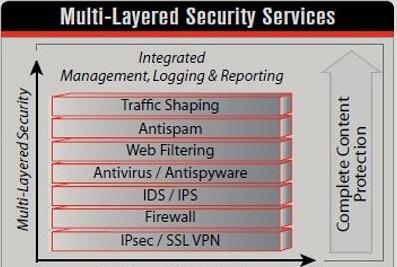
\includegraphics[width=0.8\textwidth]{gidc-sec}
	\caption{GIDC security features}
	\label{fig:gidc-sec}
\end{figure}

The Figure \ref{fig:gidc-sec} shows the different
levels of logical security for the
protection of data inside NITC. There
are seven layers of Security Services
provided by NITC including firewall
and anti-spam security. These layers
provide complete content protection
along with integrated management,
logging \& reporting.

\subsection{e-Government Master Plan}
The e-Governance Master Plan for the Government of Nepal was previously
formulated by Korea IT Industry Promotion Agency (KIPA) working with the then High Level Committee for
Information Technology (HLCIT) for the years 2007 ‐ 2011. KIPA had signed a MOU with the then High Level Commission for Information Technology (HLCIT) for the said task.

\subsubsection*{eGMP2}
After a rigorous review and analysis of the e‐Government Master Plan 2007 -- 2011 and analysis of the prevailing
policies, acts and regulations concerning ICT and e‐Governance, the team determined areas that required
intervention and update and projects that need to be implemented for e ‐ Governance to be successfully realized in
Nepal.

\subsubsection*{Four pillars of eGMP2}
\paragraph*{Sustainability}
\begin{itemize}
	\item Demand Responsive / Self-ownership Projects (Bottom Up Approach)
	\item Shared Benefits (Citizen / Business, Government / Employees, Social / Economic)
	\item Services outsourced / Local Technical Availability
	\item Assurance of AMC 
\end{itemize}

\paragraph*{Capacity building}
\begin{itemize}
	\item Awareness Campaigns (Citizen/Business) 
	\item Chief Information Officers (CIO) in every Government of Nepal (GON) Centers \& IT Cell
	\item HRD and Motivation
\end{itemize}

\paragraph*{Service delivery}
\begin{itemize}
	\item Client satisfaction surveys
	\item Rewards for accomplishes
	\item Use of new technology and media for better deliver
\end{itemize}

\paragraph*{Implementation}
\begin{itemize}
	\item Top Management Commitment
	\item Motivation for efficiency in work
\item Monitoring and Evaluation (M\&E)
\end{itemize}

\subsection{Human Resource Management Software}
\begin{framed}
	\begin{center}
		\begin{nepali}
			यो शीर्षक अस्पष्ट भएकाले कुनै सामग्री फेला पार्न सकिएन।
		\end{nepali}
	\end{center}
\end{framed}

\section{India}

\subsection{Community Information Centers}
A project of connecting the blocks of the District through ICT was launched in 2000 and accordingly a Community Information Centre (CIC) were also setup in Dibang Valley District. Under Phase-1 project, Mipi-Anini-Aliney Block was selected setup. Under various natural stress and strain, the project was completed in 2002 and have been operational since then. The main feature of the CIC has been the internet and email services provided in such mountainous and terrain geography where telephone service is a far off dream for a common man. The rural youths can now get connected to the rest of the world with a click of button and get any information needed. For example, when the CBSE results were declared, the students got their results sitting in their schools or Block Hqr within no time. Prior to setting up of CIC, they had to face the hardship of making long journeys to Roing, in Lower Dibang Valley District and then stand on long queues to know their results, or they had to wait for more than a month for the results to arrive at their school. Another benefit has been confirming train reservation status्\footnote{\url{https://dibangvalley.nic.in/egov-initiatives/cic/}}.


\subsubsection*{Objectives}
The project aims to achieve the following objectives:

\begin{multicols}{2}
	\begin{itemize}
		\item ICT Infrastructure at Block level
		\item Web Access and Internet Services such as E-mail
		\item Market Access and E-commerce
		\item Access to Socio-Economic Databases
		\item E-learning (Computer Aided Learning Processes) and E-education
		\item E-medicine, E-consulting
		\item E-governance applications, Government to Citizen (Citizen Centric) services
		\item Weather Information
		\item IT awareness among local people
		\item Computer Training Programmes
		\item Tender Notification
		\item E-employment Notification
	\end{itemize}
\end{multicols}

\subsubsection*{Infrastructure and Management}
The Centre is well-equipped with infrastructure including one server machine, five client systems, one each of a VSAT, Laser Printer, Dot Matrix Printer, modem, LAN hub, TV, Webcam and two UPS (1KVA, 2 KVA). The CIC is looked after by CIC Operators (CICOs) for managing the centres and providing services to the public.

The project is a joint effort by Department of Information Technology (DIT) under Ministry of Communications and Information Technology (MCIT, now Ministry of Electronics \& Information Technology-MEITY), National Informatics Centre (NIC) and the State Governments of the North-Eastern states.

DIT  funded the project and had the responsibility of overall monitoring and management. NIC was the Implementation agency. Application Software development and Training of CIC Operators were a part of NIC’s responsibilities. The State Governments were entrusted with the mandate of site selection, preparation and maintenance, manpower recruitment and identification and creation of content for various services/applications to be delivered through the CIC.

\subsubsection*{Future Plans}
It is proposed to use the Community Information Centres for e-Entertainment in the future. A select bouquet of channels could be telecast through the VSAT based network as TVs with other associated infrastructure is already available at the CIC. Other future prospects are the provision of connectivity to Schools and Block Offices.

\subsection{e-Procurement in The Government of Andhra Pradesh}
The state of Andhra Pradesh identified e-procurement as a core e-government project with a view to introducing transparency and accountability in its procurement operations which amount to about \(\$ 2\) billion (\textnp{२ अरब डलर}) annually. It is decided to adopt a \gls{ppp} model for implementation of the concept. After evaluating the proposals of the 12 e-procurement players in the world, it selected the affiliate of Commerce One in India — C1 India Ltd.\ — to implement the project.

C1 India, set up the required infrastructure and hosted the e-procurement marketplace. Initially, four major procuring agencies, dealing with public works, medicines, computers and transportation were selected for the pilot. The scope of the pilot includes registration of suppliers, market making, training of the suppliers and employees of the buying agencies and introduction of end-to-end procurement capabilities in the portal. The current features include online notification of all tenders, online filing of tenders, auctions and reverse auctions. The partner gets compensated at a fixed percentage of the value of goods and services procured.

The e-Procurement project of Andhra Pradesh, went on to expand its purview to serve over \(90\%\) of the procurement Government. It evolved into a sophisticated system with enhanced security features, analytical capabilities and a digital signature requirement that is mandatory for all users-buyers and suppliers as well. The project continues to be vibrant and is serving the increasing online procurement needs of the Government.

\subsection{e-Suvidha}
E-Suvidha Project has been envisaged with the main aim of benefiting urban citizens at each district of the state and to offer various governmental services both at city as well as district level within the state. Its main objectives are as follows:

\begin{itemize}
	\item To provide ‘Single window all utilities’ system at all the counters of the systematic and well integrated Citizen Service Centres (E-Suvidha Centre) installed at prime locations within the state adjacent to public houses and workplaces that offers computerized information regarding various government departments, semi-government departments, institutional departments, authorized organizations, self-financing departments, integrated information related to selected corporations and bodies, allows settlement of bills, Government payments (G2C) and  professional services of private entities (B2C) through the use of information technology.

	\item To benefit the urban citizens with the above stated services in all the districts of the state and to offer various governmental services both at city and district level.
\end{itemize}

This project has been established as the subordinate official society of \gls{it} and Electronics Department, Government of Uttar Pradesh under Societies Registration Act 1860, and is popularly known as E-Suvidha.

Under E-Suvidha Project citizens are offered various bill payment services of different departments all at one place i.\ e.\ at e-suvidha centre where ‘Single Window all Utilities’ system is followed whereby citizens don’t have to visit different departments for submitting the bills. Presently, this facility is operated through setting up of intranet but in near future it has been proposed that all the services would be made available to the citizens on their residences only via internet.


\subsubsection*{Vision}
The vision of e-Suvidha project is “to provide to the citizens of Uttar Pradesh, all G2C and G2B   One-Stop services and information of Departments and agencies of Central, State and Local Governments in an efficient, reliable, transparent and integrated manner on a sustained basis, with certainty, through easy access to a chain of computerized Integrated Citizen Service Centers (ICSC’s) and through multiple delivery channels like Electronic Kiosks, mobile phones and the Internet”.
The vision of e-Suvidha is to eventually bring all the G2C, G2B and B2C services within the purview of the project as a single interface to obviate the need for citizens and business people to visit the Government offices except for specialized and complex services

% \subsubsection*{Mission}
% The Mission of e-Suvidha Project is “to be the One-Stop-Shop for all C2G interactions”.

% \

\subsubsection*{e-Suvidha Services}
\paragraph*{G2C Services}

\begin{multicols}{2}
	\begin{itemize}
		\item Revenue Department
		\item Urban Development Department
		\item Medical \& Health Department
		\item Social Welfare Department
		\item Women Welfare \& Child Development Department
		\item Handicap Welfare Department
		\item Employment Department
		\item Food \& Civil Supplies Department
		\item Panchayati Raj Department
		\item Labour Board
		\item All Concerned departments with respect to e-District
	\end{itemize}
\end{multicols}


\paragraph*{B2C Services}
\begin{multicols}{2}
	\begin{itemize}
		\item PAN Card
		\item Aadhar Card
		\item LIC Premium Collection
		\item Mobile Top-up/Recharge
		\item Internet Data Card Recharge
		\item Mobile bills payment
	\end{itemize}
\end{multicols}


\section{Other Countries}
\begin{framed}
	\begin{center}
		\begin{nepali}
			परीक्षा नजिकिएकाले यी शीर्षक भित्रका कुनै पनि सामग्री खाेजतलास गरिएन।
		\end{nepali}
	\end{center}
\end{framed}

\subsection{E-Government Development in South Korea}
Assignment

\subsection{e-Government in China}
Assignment

%Although China is not among the top 50 in the United Nation’s 2012 ranking of national e-
%government performance—it ranks 78th—Chinese leadership has increasingly encouraged e-
%government programs, which have outpaced China’s economic and demographic peers. In
%2012, a UN survey labeled China’s e-government gains “impressive.”
%
%Chinese e-government may also help address the staggering disparity between rural and urban
%Chinese. Many commentators argue that the large gaps between rural and urban income,
%services and infrastructure in China—some of the world’s most drastic—can be addressed by
%closing the “digital divide” between the two regions.
%
%Central government is employing the Internet as an instrument to assist or accelerate the
%process of reformation and to efficiently implement some political measures. The e importance
%of e-government in China is now acknowledged. By introducing a rational and transparent e-
%government, the Chinese government has taken a significant step towards technical legitimacy,
%even if the government’s fate cannot be predicted.
%E-government services are now available in more than 90 percent of China's cities and 80
%percent of its towns, Vice President of the Chinese Academy of Governance Hong Yi said
%Thursday.
%
%All central government departments and provincial-level governments have established
%websites and 99.1 percent of municipal governments have done the same. Over 90 percent of
%core central government services, such as those relating to customs, taxation, public security
%and social security, are now offered online.
%
%Chinese e-government services have seen progress in terms of networking, infrastructure,
%digitalization, sharing and security over the last decade
%Despite several efforts in recent years, weak infrastructure and poor education levels of the
%rural population have continued to hamper the promotion of the Internet in the countryside,
%Therefore, the Chinese Government was now exploring different and more pragmatic methods
%to improve e-governance in these areas, rather than merely trying to spread the use of the
%Internet.


\subsection{e-Government in Brazil}
Assignment

\subsection{e-Government in  Sri Lanka}
Assignment

%The Government Information Centre (GIC) was established as Sri Lanka’s first one-stop
%Government call centre under the Re-engineering Government Programme in August, 2006 to
%enable citizens to obtain Government information and services in an efficient, effective and
%friendly manner. The GIC was launched as a public / private sector partnership and it is
%a single, electronic, trilingual, online knowledgebase of over 1,500 services available from more
%than 120 key Government organizations.
%
%By using GIC (call centre), general public can obtain accurate information immediately. It is
%easy, time saving and the information about many services can be obtained from one place.
%There is no need to visit Government institutes to get information, no need to wait and waste
%time in institutions to obtain information; hence it saves time and expenses during the visits.
%Ultimately the GIC helps people to make their day to day work easier by minimizing the burden
%of obtaining information on Government services.
%
%The Government of Sri Lanka (GoSL) launched “e-Sri Lanka”, a national development initiative in
%November 2002, with the aim of enhancing growth and equity through: (1) improved access
%and use of information and communication technology; (2) access to and use of public services
%on-line by businesses and citizens; and (3) enhanced competitiveness of the private sector and
%in particular of knowledge industry and small and medium enterprises (SMEs).
%
%e-Sri Lanka is a roadmap with the objective of harnessing ICTs towards achieving socio-
%economic development in the country. It is comprised of six core programmes: Re-Engineering
%Government, e-Society, ICT Policy, Leadership and Capacity Building, Information Infrastructure,
%and ICT Investment and Private Sector Development.
%
%Specifically the project work supports (1) establishing an effective, citizen centered and
%business friendly government; (2) empowering the rural poor, disadvantaged groups, women
%and youth through increased and affordable access to information and communication tools
%developing leadership and skills in ICT; and (3) creating employment in the ICT industry and ICT
%enabled services, and enhancing the competitiveness of user industries and services.
%The project comprises the following component Programmes:
%
%- ICT Policy, Leadership and Institutional Development Programme
%- ICT Human Resource Development and Industry Promotion Programme
%- Backbone Communications Infrastructure
%- Tele-Centre Development Programme
%Re-engineering Government Programme
%- e-Society Programme
%
%Government Organizations are the main stakeholders of GIC project. At present over 120
%Government Institutes are linked with GIC and the information on services of those
%organizations are available in GIC knowledgebase. GIC activities in Government Organizations
%are coordinated through a “GIC Coordinator”, who is appointed by the organization.
%
%After the introduction of GIC, positive changes have been observed in providing Government
%services to general public. Other than public awareness on Government Organizations and its
%services, other changes have not been very significant but still the changes show a positive
%impact on the Government Sector

\subsection{e-Government in  Singapore}
Assignment

\subsection{e-Government in  USA}
Assignment



\newpage\thispagestyle{empty}


 % ch-9: Case Studies \& Applications 
%%%%%%%%%%%%%%%%%%%%%%%%%%%%%%%%%%%%%%%%%%%%%%%%%%%%%%%%%%%%%%%%%%%%%%

% questions
\cleardoublepage
\phantomsection
\addcontentsline{toc}{chapter}{Questions (2018 \& 2019)}

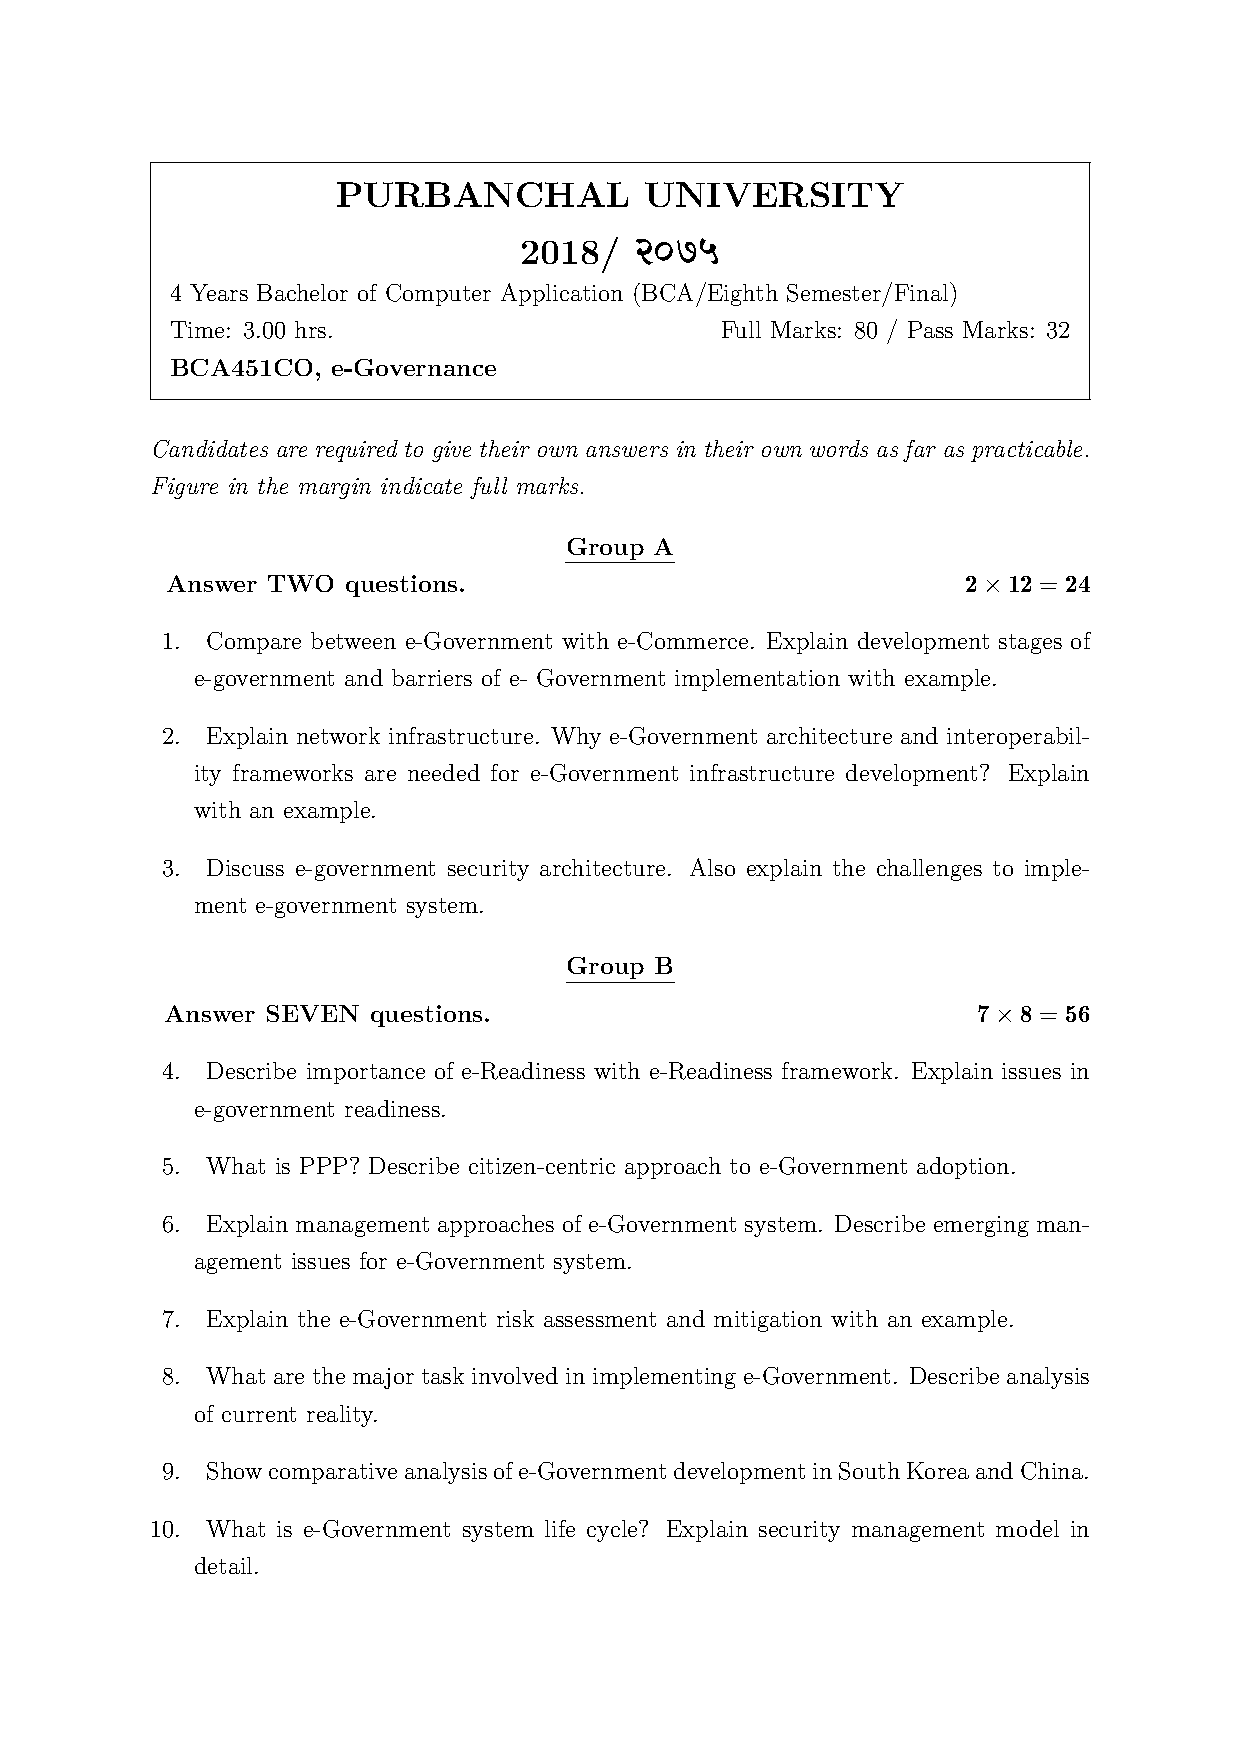
\includepdf[pagecommand={\thispagestyle{plain}}, pages={1-6}, scale=1.0]{./questions/build_dir/e_gov_questions}



\backmatter


 \nocite{*}
 \renewcommand{\bibname}{References}
 \phantomsection
 \addcontentsline{toc}{chapter}{References} % add References to toc
 \printbibliography %prints bibliography list
 


\end{document}
